\documentclass{book}
\usepackage{graphicx} 
\usepackage{amsmath}
\usepackage{amssymb}
\usepackage{amsthm}
\usepackage{subcaption}
\usepackage[export]{adjustbox}
\usepackage{graphicx}
\usepackage{tikz}
\usepackage{makeidx}
\usepackage{wrapfig}
\usepackage{multicol,lipsum}
\usetikzlibrary{arrows.meta}
\usetikzlibrary{calc}
\usepackage{hyperref}
\usepackage[
backend=biber,
style=alphabetic,
sorting=ynt
]{biblatex}
\addbibresource{references.bib}

\title{Notes of Field and Service Robotics}
\author{Carlo Alberto Giacchetti, Alessandro Prisco}
\date{August 2025}

\usepackage[
    a4paper,
    left=2cm,   % Margine sinistro
    right=2cm,  % Margine destro
    top=2.5cm,  % Margine superiore
    bottom=2.5cm, % Margine inferiore
    % includeheadfoot % Opzionale: include intestazione e piè di pagina nel calcolo
]{geometry}

\begin{document}
\setcounter{secnumdepth}{3}
\setcounter{tocdepth}{3}

\makeatletter
\let\oldendproof\endproof
\def\endproof{\oldendproof\aftergroup\@afterindentfalse\aftergroup\@afterheading}

\newtheorem{theorem}{Theorem}
\newtheorem{lemma}{Lemma}[section]
\theoremstyle{definition}
\newtheorem{definition}{Definition}[section]
\makeatother
\maketitle
\makeatletter
\renewcommand*\env@matrix[1][\arraystretch]{%
  \edef\arraystretch{#1}%
  \hskip -\arraycolsep
  \let\@ifnextchar\new@ifnextchar
  \array{*\c@MaxMatrixCols c}}
\makeatother
\tableofcontents

\newpage
\maketitle
\newpage

\chapter{Introduction}
    By the term \textit{Mobile robots} it is meant an ensemble of rigid bodies, equipped with a locomotion system. It is then understood that the ability of freely moving around their environment is the biggest difference between mobile and industrial robots, the latter being mostly bolted to the ground. \\
    Mobile robots are mainly distinguished by their locomotion systems:
    \begin{itemize}
        \item \textit{Wheeled Robots}: composed by one rigid body, the \textit{chassis}, to which wheels are attached (and trailers if needed).
        \item \textit{Legged Robots}: multiple rigid bodies, some of which mimic legs. The robot has multiple extremities (\textit{feet}) in periodic contact with the ground to achieve motion.
        \item \textit{Flying Robots}: composed by a rigid body, the \textit{frame}, to which either rotors or fixed wings are attached. Propellers represent the locomotion system.
        \item \textit{Underwater Robots}: very similar to flying robots, but with the additional care due to the environment in which they work.
    \end{itemize}
    Building mobile robots comes with some challenges, such as:
    \begin{itemize}
        \item \textit{Localization} in their (dynamic or static) environment; mobile robots can make use of encoders and GPS, but these either have many unmodelled dynamics or flat-out don't work in some environments and situations. Another complication is computational: Direct Kinematics is expressed by (often constrained) sets of differential equations. 
        \item State-Estimation or \textit{Odometry} is also very complex and has the goal of estimating the robot's position from either on-board or off-board sensors; often robots perform \textit{Simultaneous Localization And Mapping} (SLAM) online during execution of their tasks, making Odometry a very computationally heavy task.
        \item \textit{Motion Planning} is the job of computing a path and time law (a \textit{trajectory}) compatible with the environment. This is often done in real-time for mobile robots, making it again very difficult for the designer.
        \item \textit{Motion Control} is the task of determining the robot's inputs to follow the planned path. This is difficult because, opposite to industrial robotics, there are plenty unmodelled dynamic effect taking action on a mobile robots, some of which could not even be envisioned before deploying the robot itself.
        \item Last but not least, the control \textit{Architecture} has to be chosen. There are mainly four approaches:
        \begin{itemize}
            \item \textit{Reactive Architecture}: "don't think, act".
            \item \textit{Hybrid Architecture}: Think and Act simultaneously.
            \item \textit{Behavioural Architecture}: Think about the action modality.
            \item \textit{Deliberative Architecture}: Think, then act. This is the one adopted in this course, based on Propioceptive and Exteroceptive sensors and perception.
        \end{itemize}
    \end{itemize}
    \section{Configuration Space and Degrees of Freedom}
    As previously stated, a mobile robot is free to move in its environment, which immediately begs the question of how to describe such a system.
     The robot’s \textbf{configuration} is the specification of the positions of all points of the robots, which will be assumed as the interconnection of fully rigid links by means of joints. This simplification greatly reduces the number of parameters needed to describe the robot's full configuration; then, the minimum number of real-valued coordinates needed to represent the configuration is called \textit{Degrees Of Freedom} of the system. By merging the two definitions, the \textit{Configuration Space} of a robot can be defined as:
    \begin{definition}
        \textbf{Configuration Space}: The $n$-dimensional space, where $n$ is the robot's number of DoFs, containing all the possible robot's configurations is called the \textit{Configuration Space} (C-space). The configuration of a robot is represented by a point in its C-space.
    \end{definition}
    An unconstrained rigid body immersed in three dimensional space has 6 DoFs (3 translational and 3 rotational), meanwhile in 2D space it has only 3 (2 translational and 1 rotational), as is known from physics. In general, a simple formula for computing the number of DoFs is:
    \begin{gather*}
        \text{DoFs}=(\text{Sum of degrees of freedom of the single bodies})+\\-(\text{number of independent constraints})
    \end{gather*}
    This formula can be easily applied on mechanical systems, such as robots, and takes the name of \textit{Gr\"{u}bler's Formula}:
    \begin{definition}
        \textbf{Gr\"{u}bler's Formula}: Consider a mechanism of $N$ links, counting also the ground. Let $J$ be the number of joints, $m$ the DoFs of a rigid body in the considered space, $f_i$ the DoFs provided by joint $i$ and $c_i$ the number of constraints provided by joint $i$, where $f_i+c_i=m$, for all $i$. Then, the number of DoFs of the robot is at least: 
        \begin{equation}\label{Grubler's formula}
            DoFs = m(N-1)-\sum_{i=1}^{J}c_i=m(N-1-J)+\sum_{i=1}^{J}f_i
        \end{equation}
        The equation is exact in the case of fully independent constraints, otherwise it is a \textbf{lower bound} for the number of DoFs of the mechanism.
    \end{definition}
    Different joints can give different DoFs based on their structure; in the following table, the most famous joints and their respective characteristic are summarized:
   \begin{figure}[htbp!]
    \centering
    \begin{minipage}{0.48\textwidth}
        \centering
        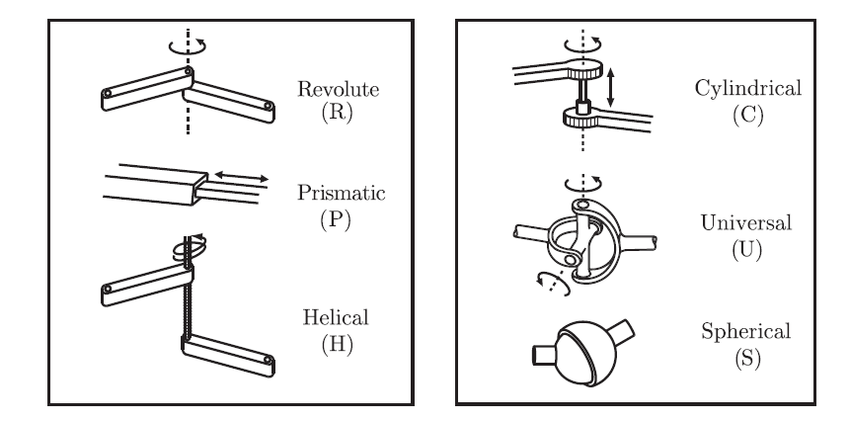
\includegraphics[width=\linewidth]{Images/typical_robot_joints.png}
    \end{minipage}\hfill
    \begin{minipage}{0.48\textwidth}
        \centering
        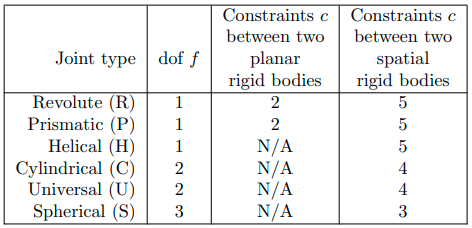
\includegraphics[width=\linewidth]{Images/image2.png}
    \end{minipage}
    \caption{Table of joints' characteristics.}
    \label{fig:joints_charas}
\end{figure}\\
\newpage
\subsection{Gr\"{u}ber's Formula examples}
    Let's see some examples of how to use Gr\"{u}bler's formula.
    \begin{itemize}
    \item Four bar Linkage \\
    
    
 \begin{figure}[htbp!]
                \begin{minipage}{0.4\textwidth}
                    We have 4 Links (considering the ground link) and 4 \textit{Revolute} Joints. We are considering the model in the plane, thus we have that 
\[
 N=4 (\text{four links}), J = 4 (\text{four joints}), m = 3 (\text{plane}),
 \]\[ f_i = 1 (\text{Revolute Joints in the plane})              
                    \]   
                    By applying Gruber's rule
                    \[DoFs=3(4-1-4)+4 = 1\]
                 
                \end{minipage}\hfill
                \begin{minipage}{0.5\textwidth}
                    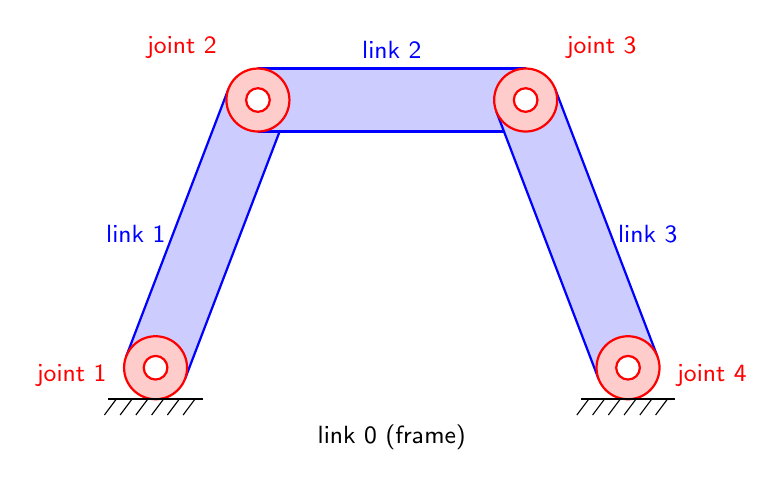
\begin{tikzpicture}[>=stealth]

    % Definizione delle coordinate dei 4 giunti
    \coordinate (A) at (0,0);
    \coordinate (B) at (1.3, 3.4);
    \coordinate (C) at (4.7, 3.4);
    \coordinate (D) at (6,0);

    % Macro per disegnare i bracci di collegamento (Link - BLU)
    \newcommand{\drawlink}[2]{
        % Riempimento azzurro chiaro
        \fill[blue!20] ($(#1)!4mm!-90:(#2)$) -- ($(#2)!4mm!90:(#1)$) -- 
                       ($(#2)!4mm!-90:(#1)$) -- ($(#1)!4mm!90:(#2)$) -- cycle;
        % Bordi blu
        \draw[thick, blue] ($(#1)!4mm!-90:(#2)$) -- ($(#2)!4mm!90:(#1)$);
        \draw[thick, blue] ($(#1)!4mm!90:(#2)$) -- ($(#2)!4mm!-90:(#1)$);
    }

    % Macro per disegnare i supporti a terra (Telaio - NERO)
    \newcommand{\ground}[1]{
        \begin{scope}[shift={(#1)}]
            \draw[thick] (-0.6, -0.4) -- (0.6, -0.4);
            \foreach \i in {-0.5, -0.3, -0.1, 0.1, 0.3, 0.5} {
                \draw (\i, -0.4) -- (\i-0.15, -0.6);
            }
        \end{scope}
    }

    % 1. Disegno i tre bracci (collegamenti) - Colore BLU
    \drawlink{A}{B}
    \drawlink{B}{C}
    \drawlink{D}{C}

    % 2. Disegno i giunti (cerchi esterni e perni interni) - Colore ROSSO
    \foreach \p in {A,B,C,D} {
        % Cerchio esterno con riempimento rosso chiaro e bordo rosso
        \filldraw[thick, draw=red, fill=red!20] (\p) circle (4mm);
        % Perno interno con bordo rosso e riempimento bianco
        \filldraw[thick, draw=red, fill=white] (\p) circle (1.5mm);
    }

    % 3. Disegno i supporti a terra nei punti A e D
    \ground{A}
    \ground{D}

    % ==========================================
    % 4. ETICHETTE (LABELS) COLORATE
    % ==========================================
    
    \tikzset{etichetta/.style={font=\sffamily\small}}

    % Etichette per i giunti (Rosse)
    \node[etichetta, text=red, anchor=east]       at ($(A) + (-0.5, -0.1)$) {joint 1};
    \node[etichetta, text=red, anchor=south east] at ($(B) + (-0.4,  0.4)$) {joint 2};
    \node[etichetta, text=red, anchor=south west] at ($(C) + ( 0.4,  0.4)$) {joint 3};
    \node[etichetta, text=red, anchor=west]       at ($(D) + ( 0.5, -0.1)$) {joint 4};

    % Etichette per i bracci (Blu)
    \path (A) -- (B) node[midway, left=0.4cm, etichetta, text=blue] {link 1};
    \path (B) -- (C) node[midway, above=0.4cm, etichetta, text=blue] {link 2};
    \path (D) -- (C) node[midway, right=0.4cm, etichetta, text=blue] {link 3};
    
    % Etichetta per il telaio (Nera)
    \path (A) -- (D) node[midway, below=0.6cm, etichetta] {link 0 (frame)};

\end{tikzpicture}
                \end{minipage} 
            \end{figure} 
Now here it comes the most complex part: understanding the presence of dependent constraints. By reasoning about the model we can notice that by moving just one joint, the position of all the other joints is imposed, thus we showed that the number of DoFs is properly one.
\item Slider-Crank \\
   
 \begin{figure}[htbp!]
                \begin{minipage}{0.4\textwidth}
                    We have 4 Links (considering the ground link) and 4 \textit{Revolute} Joints. We are considering the model in the plane, thus we have that 
\[
 N=4 (\text{four links}), J = 4 (\text{four joints}), m = 3 (\text{plane}),
 \]\[ f_i = 1 (\text{3 Revolute and 1 prismatic})              
                    \]   
                    By applying Gruber's rule
                    \[DoFs=3(4-1-4)+4 = 1\]
                 
                \end{minipage}\hfill
                \begin{minipage}{0.5\textwidth}
                    
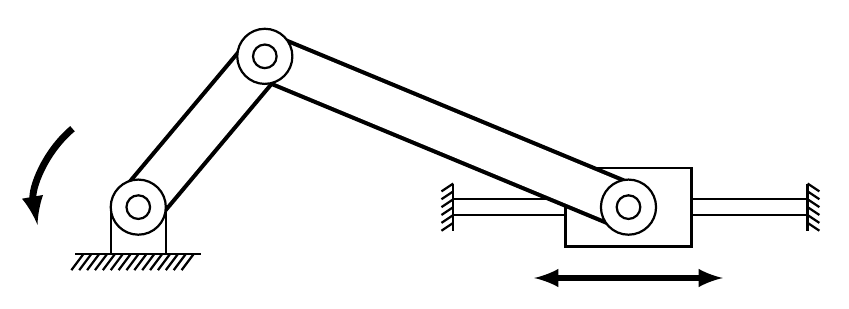
\begin{tikzpicture}[>=latex]

    % === Parametri del meccanismo ===
    \def\crankangle{50}   % Angolo della manovella
    \def\cranklen{2.5}    % Lunghezza manovella (OA)
    \def\rodlen{5}        % Lunghezza biella (AB)

    % === Calcolo delle coordinate ===
    % O: Perno fisso (origine)
    \coordinate (O) at (0, 1);
    % A: Perno manovella-biella
    \coordinate (A) at ({\cranklen*cos(\crankangle)}, {1 + \cranklen*sin(\crankangle)});
    % B: Perno del cursore (intersezione asse orizzontale)
    \pgfmathsetmacro{\Bx}{\cranklen*cos(\crankangle) + sqrt(\rodlen^2 - (\cranklen*sin(\crankangle))^2)}
    \coordinate (B) at (\Bx, 1);

    % === 1. Guide fisse e Asta del cursore (sullo sfondo) ===
    % Asta orizzontale
    \draw[thick] (4.0, 0.9) -- (8.5, 0.9);
    \draw[thick] (4.0, 1.1) -- (8.5, 1.1);
    
    % Guida fissa sinistra (con tratteggi)
    \draw[thick] (4.0, 0.7) -- (4.0, 1.3);
    \foreach \y in {8, 9, 10, 11, 12, 13} {
        \draw[thick] (4.0, \y/10) -- (3.85, \y/10 - 0.1);
    }
    
    % Guida fissa destra (con tratteggi)
    \draw[thick] (8.5, 0.7) -- (8.5, 1.3);
    \foreach \y in {8, 9, 10, 11, 12, 13} {
        \draw[thick] (8.5, \y/10) -- (8.65, \y/10 - 0.1);
    }

    % === 2. Base del perno fisso (O) e Terra ===
    \draw[thick, fill=white] (-0.35, 0.4) -- (-0.35, 1) -- (0.35, 1) -- (0.35, 0.4) -- cycle;
    \draw[thick] (-0.8, 0.4) -- (0.8, 0.4); % Linea di terra
    \foreach \x in {-7, -6, -5, -4, -3, -2, -1, 0, 1, 2, 3, 4, 5, 6, 7} {
        \draw[thick] (\x/10, 0.4) -- (\x/10 - 0.15, 0.2); % Tratteggi terra
    }

    % === 3. Blocco Cursore (Slider) ===
    \draw[thick, fill=white] ($(B)+(-0.8,-0.5)$) rectangle ($(B)+(0.8,0.5)$);

    % === 4. Biella (Collegamento AB) ===
    % Disegniamo una linea spessa nera e ci sovrapponiamo una linea bianca un po' più sottile
    \draw[line width=18pt, black, line cap=round] (A) -- (B);
    \draw[line width=15pt, white, line cap=round] (A) -- (B);

    % === 5. Manovella (Collegamento OA) ===
    % Disegnata dopo la biella in modo da sovrapporsi a essa sul giunto A
    \draw[line width=18pt, black, line cap=round] (O) -- (A);
    \draw[line width=15pt, white, line cap=round] (O) -- (A);

    % === 6. Giunti / Perni di collegamento ===
    % Cerchi esterni (coprono le imperfezioni e creano le "teste" dei bracci)
    \draw[thick, fill=white] (O) circle (0.35);
    \draw[thick, fill=white] (A) circle (0.35);
    \draw[thick, fill=white] (B) circle (0.35);

    % Cerchi interni (i veri e propri perni)
    \draw[thick] (O) circle (0.15);
    \draw[thick] (A) circle (0.15);
    \draw[thick] (B) circle (0.15);

    % === 7. Frecce di indicazione movimento ===
    % Freccia di rotazione (Manovella)
    \draw[line width=2.5pt, -latex] ($(O)+(130:1.3)$) arc (130:190:1.3);

    % Freccia di traslazione (Cursore)
    \draw[line width=2pt, latex-latex] ($(B)+(-1.2,-0.9)$) -- ($(B)+(1.2,-0.9)$);

\end{tikzpicture}
                \end{minipage} 
            \end{figure} 

        \item A mechanism with overlapping joints:
            \begin{figure}[htbp!]
                \begin{minipage}{0.4\textwidth}
                    \centering                  
                    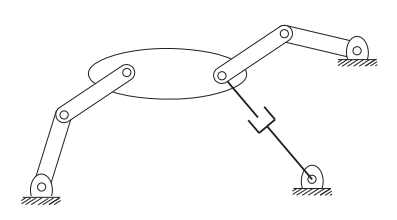
\includegraphics[width=\textwidth]{Images/image1.png}
                    \caption{Planar mechanism with \\ overlapping joints.}
                    \label{fig:mech_overlapping}
                \end{minipage}\hfill
                \begin{minipage}{0.5\textwidth}
                    The planar mechanism illustrated in fig: \ref{fig:mech_overlapping} has three links that meet at a single point on the right of the large link. Recalling that a joint by definition connects exactly two links, the joint at this point of intersection should not be regarded as a single revolute joint. Rather, it is correctly interpreted as two revolute joints overlapping each other. There is more than one way to derive the number of degrees of freedom of this mechanism using Gr\"{u}bler's formula: 
                \end{minipage} 
            \end{figure} 
            \begin{itemize}
                    \item i) The mechanism consists of eight links ($N = 8$), eight revolute joints and one prismatic joint ($J=9$). Substituting this into the formula yields: 
                    \begin{equation*} 
                        DoFs = 3(8-1-9)+9(1)=3
                    \end{equation*}
                    \item ii) Alternatively, the lower-right revolute–prismatic joint pair can be regarded as a single two-DoFs joint. In this case the number of links is $N = 7$, with seven revolute joints, and a single two-DoFs revolute–prismatic pair. Substituting into the formula:
                    \begin{equation*}
                        DoFs=3(7-1-8)+7(1)+1(2)=3
                    \end{equation*}
            \end{itemize}
        \item (Redundant constraints and singularities)
            \begin{figure}[htbp!]
                \centering
                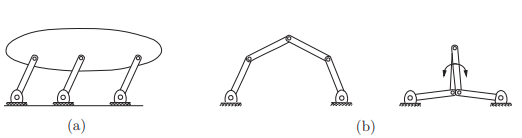
\includegraphics[width=0.5\linewidth]{Images/image3.png}
                \caption{(a) A parallelogram and (b) five-bar (in a regular and singular configuration) linkages}
                \label{fig:placeholder}
            \end{figure} \\
            For the parallelogram linkage, $N = 5, J = 6$, and $f_i = 1$ for each joint. From Gr\"{u}bler’s formula, the number of degrees of freedom is:
            \[3(5-1-6) + 6 = 0\]
            A mechanism with zero degrees of freedom is by definition a rigid structure. It is clear from examining the figure, though, that the mechanism can in fact move with one degree of freedom. Indeed, any one of the three parallel links, with its two joints, has no effect on the motion of the mechanism, so we should have calculated $DoFs = 3(4-1-4) + 4 = 1$. In other words, the constraints provided by the joints are not independent, as required by Gr\"{u}bler’s formula. \\
            A similar situation arises for the two-DoFs planar five-bar linkage: if the two joints connected to ground are locked at some fixed angle, the five-bar linkage should then become a rigid structure. However, if the two middle links are the same length and overlap each other, these overlapping links can rotate freely about the two overlapping joints.
            \newpage
        \item Delta Robot:
            \begin{figure}[htbp!]
                \begin{minipage}{0.4\textwidth}
                    \centering                  
                    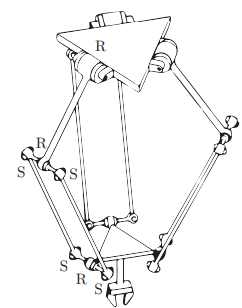
\includegraphics[width=\textwidth]{Images/image4.png}
                    \caption{Delta Robot}
                    \label{fig:delta_robot}
                \end{minipage}\hfill
                \begin{minipage}{0.5\textwidth}
                    The Delta robot consists of two platforms – the lower one mobile, the upper one stationary – connected by three legs. Each leg contains a parallelogram closed chain and consists of three revolute joints, four spherical joints, and five links. Adding the two platforms, there are $N = 17$ links and $J = 21$ joints (nine revolute and 12 spherical). By Gr\"{u}bler’s formula:
                    \[DoFs=6(17-1-21)+9(1)+12(3)=15\]
                    However, only three DoFs are actually visible from the end-effector perspective; this is one of the many perks of this robot, since it is capable of always maintaining its two platforms parallel to each other.
                \end{minipage} 
            \end{figure} 
        \end{itemize}
        Up until now we have only considered the dimension of the Configuration Space, i.e. the Degrees of Freedom; however, there is another aspect of great importance: the topology\footnote{In the context of pure mathematics, a \textit{topology} over a set $X$ is just a collection of sets, $\tau$, which are called \textit{open sets}, such that:
        \begin{itemize}
            \item $\emptyset,X\in \tau$ 
            \item If $O_i,O_j \in \tau$, then $O_i\cap O_j\in\tau$, for all $O_i,O_j \in \tau$.
            \item If $\mathcal{O}\subseteq \tau$, then $\cup_{O\in\mathcal{O}}O\in\tau$
        \end{itemize}
        Then, the couple $(X,\tau)$ is called a \textit{Topological Space}.}. \\
        Consider a plane and the surface of a sphere; to completely specify the position of a point in both spaces, there is need for only two coordinates (the $x,y$ coordinates in the plane or the longitude/latitude on the sphere), however the \textit{shape} of the two spaces is different: coordinates can wrap around on the surface of a sphere, meanwhile they cannot on the plane. Two spheres can be, however, be thought of as "the same" just deformed and are called \textit{topologically equivalent}; 
        \section{Topology Definition}
        A topological space can be expressed through different kind of definition. The main elements of topology are the open sets, the neighbourhoods and the points.
         More specifically, a topological space is a set whose elements are called points, along with an additional structure called a topology, which can be defined as a set of neighbourhoods for each point that satisfy some axioms formalizing the concept of closeness. There are several equivalent definitions of a topology, the most commonly used of which is the definition through open sets. 
         a topological space is, roughly speaking, a geometrical space in which closeness is defined but cannot necessarily be measured by a numeric distance.
        \begin{definition}
            \textit{Topological Equivalence}: A function $f:X \rightarrow Y$ between two topological spaces is a \textit{homeomorphism} if: 
            \begin{itemize}
                \item $f$ is a bijection.
                \item $f$ is continuous.
                \item $f^{-1}$ is continuous.
            \end{itemize}
            If such a function exists, then $X$ and $Y$ are \textit{topologically equivalent}. Geometrically, this means that one topological space can be continuously deformed into the other without cutting or adding any elements.
        \end{definition}
        As an example, the open set $(a,b)\subseteq \mathbb{R}$ is topologically equivalent to a line of real numbers by first folding it into a semicircle and then assigning its points to a line, as in the figure below.
        \begin{figure}[h!]
            \centering
            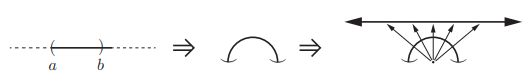
\includegraphics[width=0.5\linewidth]{Images/image5.png}
            \caption{: An open interval of the real line, denoted (a, b), can be deformed to an open semicircle. This open semicircle can then be deformed to the real line by the mapping illustrated: beginning from a point at the center of the semicircle, draw a ray that intersects the semicircle and then a line above the semicircle. These rays show that every point of the semicircle can be stretched to exactly one point on the line, and vice versa. Thus an open interval can be continuously deformed to a line, so an open interval and a line are topologically equivalent.
            }
            \label{fig:open_set_into_line}
        \end{figure}\\
        However, a closed set \textit{is not} topologically equivalent to a line, since it ends, the line does not. Note that the topology of a space is a fundamental property of the space itself and \textit{is independent} of how we choose coordinates to represent points in the space.
        Some C-spaces can be expressed as the Cartesian product of two or more spaces of lower dimension; that is, points in such a C-space can be represented as the union of the representations of points in the lower-dimensional spaces. For example:
        \begin{itemize}
            \item The C-space of a rigid body in the plane can be written as $\mathbb{R}\times S^1$, where $S^n$ is the surface of a $n$-dimensional space immersed into $(n+1)$-dimensional space.
            \item As we saw when we counted the degrees of freedom of a rigid body in three dimensions, the configuration of a rigid body can be described by a point in $\mathbb{R}^3$, plus a point on a two-dimensional sphere $S^2$, plus a point on a one-dimensional circle $S^1$, giving a total C-space of $\mathbb{R}^3 \times S^2 \times S^1$.
            \item The C-space of a PR robot arm can be written as $\mathbb{R}\times S^1$ (ignoring joints limits). 
        \end{itemize}
        While it is natural to choose a reference frame and length scale and to use a vector to represent points in a Euclidean space, representing a point on a curved space, such as a sphere, is less obvious. A choice of $n$ coordinates, or parameters, to represent an $n$-dimensional space is called an \textit{Explicit Parametrization} of the space. Such an explicit parametrization is only valid for a particular range of the parameters; there exists \textit{singularities} in parametric parametrizations. One such example is the North (or South) Pole of a sphere over which longitude-latitude coordinates are used; in these points, the coordinates wrap around their limiting values and the homeomorphism is undefined at the "wrapping" point (the inverse function is not defined). There are two ways to overcome the problem:
        \begin{itemize}
            \item Use more than one \textit{Coordinate Chart} on the space, where each coordinate chart is an explicit parametrization covering only a portion of the space such that, within each chart, there is no singularity. Then, one can simply switch between charts. If we define a set of singularity-free coordinate charts that overlap each other and cover the entire space they are said to form an \textit{Atlas}; the advantage here is:
            \begin{itemize}
                \item A minimum representation of space is maintained at all times.
            \end{itemize} 
            However the disadvantage is:
            \begin{itemize}
                \item A high amount of memory could be needed to remember each single chart.
            \end{itemize}
            \item Use an \textit{Implicit Representation}, which views the $n$-dimensional space as embedded in a Euclidean space of more than $n$ dimensions.  An implicit representation uses the coordinates of the higher-dimensional space but subjects these coordinates to constraints that reduce the number of degrees of freedom. The advantages here are:
            \begin{itemize}
                \item There are no singularities in the representation.
                \item Only one representation is needed to fully describe the space.
                \item It is way easier to find an implicit representation against an explicit one.
            \end{itemize}
            A disadvantage of this approach is that:
            \begin{itemize}
                \item The representation is constituted by a larger number of parameters than the system's number of DoFs.
            \end{itemize}
        \end{itemize}
        From now on, only implicit representations will be used.
\subsection{Exercises}
\paragraph{ProDrone a Six propellers plus two 5-DoFs arms drone:}
 \begin{figure}[htbp!]
                \begin{minipage}{0.4\textwidth}
                    \centering                  
                    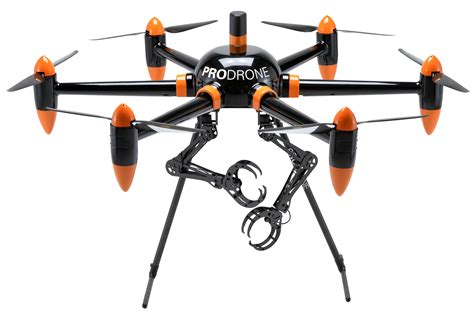
\includegraphics[width=\textwidth]{Images/ProDrone.jpg}
                    \caption{ProDrone}
                    \label{fig:ProDrone}
                    \end{minipage}
\hfill
                \begin{minipage}{0.6\textwidth}
        
\begin{itemize}
\item Body fixed on the ground
\begin{itemize}
\item 6 rotating propellers (1 link plus 1 rotational joint each)
\item 5 rotational joints for each arm
\item 1 Ground
\item DoFs = $6(6+5+5+1-1-6-5-5)+6+5+6 = 16$
\end{itemize}
\item Flying body
\begin{itemize}
\item 6 DoFs given by the spatial rigid body
\item DoFs = $16 + 6 = 22 $
\end{itemize}
\end{itemize}
                \end{minipage} 
            \end{figure}            
          
 \paragraph{Mobile Kuka a Mobile manipulator arms robot:}
 \begin{figure}[htbp!]
                \begin{minipage}{0.4\textwidth}
                    \centering                  
                    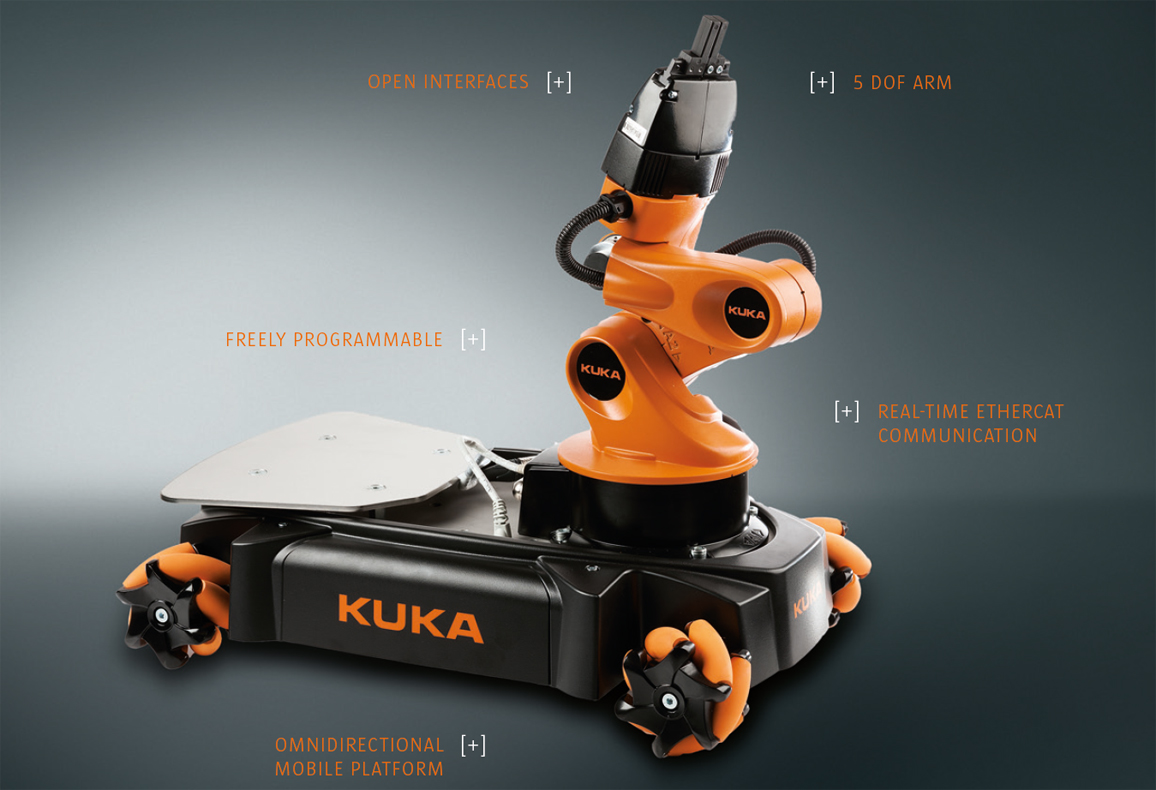
\includegraphics[width=\textwidth]{Images/Mobile_Kuka.jpg}
                    \caption{Mobile Kuka}
                    \label{fig:Mobile_Kuka}
                    \end{minipage}
\hfill
                \begin{minipage}{0.6\textwidth}
        
\begin{itemize}
\item KUKA youBot with 4 mecanum-wheels (omnidirecitonal base) plus 5-DoF robotic arm
\begin{itemize}
\item 4 wheels (1 link plus 1 rotational joint each)
\item A planar rigid body (3 DoFs)
\item 5 rotational joints for the arm
\item 12 DoFs
\end{itemize}
\end{itemize}
                \end{minipage} 
            \end{figure}
        \newpage
\section{Task space and Workspace}
        The C-space is related to the configuration of the entire robot; however, there are also other two spaces of interest, both only linked to the robot's end-effector: the \textit{Task Space} and the \textit{Workspace}. 
        \begin{definition}
            \textbf{Task Space}: The \textit{Task Space} is a space in which a robot's task can naturally be expressed.
        \end{definition}
        One example would be $\mathbb{R}^2$, a plane, for a robot whose task is to write on a sheet of paper; if the task is to manipulate a rigid body, a natural representation of the task space is the C-space of a rigid body, representing the position and orientation of a frame attached to the robot’s end-effector. This is the default representation of task space. Notice that the decision of how to define the task space \textit{is driven by the task, independently of the robot}. 
        \begin{definition}
            \textbf{Workspace}: The \textit{Workspace} is a specification of the configurations that the robot's end-effector can reach. The definition of the workspace is primarily driven by the robot’s structure, \textit{independently of the task}.
        \end{definition}
        The three spaces (Task, Work and C-space) are distinct but can overlap. A point in the task space or the workspace may be achievable by more than one robot configuration, meaning that the point is not a full specification of the robot’s configuration. For example, for an open-chain robot with seven joints, the six-DoF position and orientation of its end-effector does not fully specify the robot’s configuration. Some points in the task space may not be reachable at all by the robot, such as some points on a chalkboard. By definition, however, all points in the workspace are reachable by at least one configuration of the robot.
        \begin{figure}[htbp!]
                \begin{minipage}{0.5\textwidth}
                    \centering                  
                    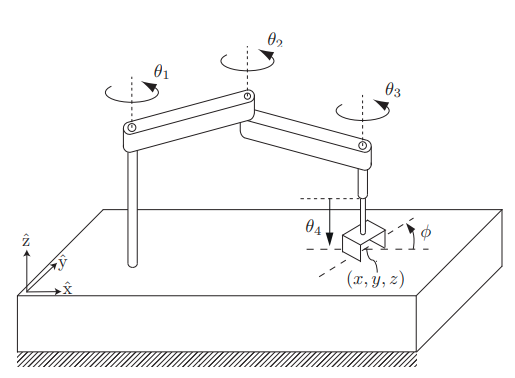
\includegraphics[width=\textwidth]{Images/image7.png}
                    \caption{SCARA Robot}
                    \label{fig:SCARA_robot}
                \end{minipage}% 
                \hfill%
                \begin{minipage}{0.5\textwidth}
                    To get an example, let's consider the SCARA robot in the picture. \\
                    The end-effector configuration is completely described by the four parameters $(x,y,z,\phi)$, where $\phi$ is the end-effector orientation in the $xy-$plane. Its task space would typically be defined as $\mathbb{R}^{3}\times S^1$, meanwhile its workspace would be typically defined as the reachable points in Cartesian space, regardless of orientation.
                \end{minipage} 
            \end{figure} 
            \section{Underactuation}
            As is known from physics, the motion of an arbitrary mechanical system occurs in such a way that the indefinite integral:
            \[A=\int_{t_i}^{t_f} \mathcal{L}(q,\dot{q})dt\]
            Called \textit{Action Integral}\footnote{There are many different definitions of \textit{action}, but this will suffice here.}, becomes stationary for all possible variations of the system's configurations, provided the initial and final state are given. The quantities $q, \dot{q}$ are called \textit{generalized coordinates} and \textit{generalized velocities} respectively, used to define the \textit{Lagrangian} $\mathcal{L}(q,\dot{q})=T-U$, where $T,U$ are the system's kinetic and potential energies. It is possible to use this definition to prove that the Action is stationary if and only if the \textit{Euler-Lagrange Equations} are satisfied: \footnote{This is \textit{Hamilton's Principle} or the \textit{Principle of Stationary Action}. A proof can be found in \cite{Taylor_ClassicalMechanics}.}
            \[\frac{d}{dt} \frac{\mathcal{\partial L}}{\partial\dot{q}}-\frac{\partial\mathcal{L}}{\partial q}=f\]
            Where $f$ is the vector of \textit{generalized forces} acting on the system. Notice that these are not necessarily forces in the classical sense of Newton's $F=ma$. \\
            The Euler-Lagrange Equations can be translated into matrix form, being completely equivalent to Newton's classic formulation of mechanics, such as:
            \[M(q)\ddot{q}+h(q,\dot{q})=f\]
            Where:
            \begin{itemize}
                \item $M(q) \in \mathbb{R}^{n \times n}$ is the \textit{Inertia Matrix}, which is positive definite and symmetric.
                \item $h(q,\dot{q})$ is the lumped vector of gravitational and non-inertial forces.
            \end{itemize}
            The relation can be inverted to extract the accelerations:
            \[\ddot{q}=-M^{-1}(q)h(q,\dot{q})+M^{-1}(q)f\]
            And if we define the generalized forces as functions of the inputs by defining the \textit{input matrix} $B$:
            \[f=B(q)\tau\]
            The system can be expressed in \textit{control-affine form}:
            \begin{equation}\label{control_affine_motion}
                \ddot{q}=b(q,\dot{q})+(M(q)^{-1}B(q))\tau=b(q,\dot{q})+G(q,\dot{q})\tau               
            \end{equation}
            Or in the general case:
            \[\ddot{q}=f(q,\dot{q},\tau,t)\]
            At this point, it should be natural to notice that it is not always the case that the control inputs can actually influence all the states, for instance in the case where the input matrix $B(q)$ is not full column-rank, meaning that the system has less inputs than states. In the general case this can be translated into a condition on the state-dynamics, in particular $f(\cdot)$ must be surjective. This is the problem of \textit{underactuation}:
            \begin{definition}
                \textbf{Underactuation}: a second order differential equation $\ddot{q}=f(q,\dot{q},\tau, t)$ is \textit{fully-actuated} in the state $x=(q,\dot{q})$ and the time $t$ if the map $f(\cdot)$ is surjective: 
                \[\forall \ddot{q}_{d}\in \mathbb{R}^{n} \exists u \in \mathbb{R}^{m}:\ddot{q}_d=f(q_0,\dot{q}_0,u,t)\]
                If this is not the case, the system is said to be \textit{underactuated}. A control-affine system is underactuated if:
                \[\text{Rank}_{\text{col}}(G(q,\dot{q}))<dim[q]\]
            \end{definition}
            It is important to notice that the system underactuation can change with either time, state or system constraints. However, usually a system is said to be underactuated if it so in every state and time. This also implies that most systems are underactuated, as for example is a quadcopter (being incapable of translating along the plane of the propellers at any time or initial state). \\
            Another keypoint about underactuation is that it depends on the mathematical model assumed for the system.  Imagine a two-link robot with two actuators. A typical model with rigid links could be fully actuated, but if we add extra DoFs to model small amounts of flexibility in the links then that system model could be underactuated. These two models describe the same robot, but at different levels of fidelity. Two actuators might be enough to completely control the joint angles, but not the joint angles and the flexing modes of the link. 
            \section{Controllability}
            Just as in linear system, in nonlinear systems it is also often useful to have a notion of \textit{controllability}.             
            \begin{definition}\label{controllability}
                \textbf{Controllability}: Let the system:
                \[\dot{x}=f(x,u)\]
                Be defined for $x \in D_{x,def}\subseteq \mathbb{R}^{n}$ and $u \in D_{u,ref} \subseteq \mathbb{R}^{m}$. Then, the system is said to be \textit{controllable} if any state $x_0 \in D_{x,def}$ can be transferred into any other $x_1 \in D_{x,ref}$ along a trajectory $x(t)\in D_{x,def}$ by an input function $u(t) \in D_{u}$ in a finite time interval $[0,T]$.
            \end{definition}
            Obviously, proving controllability for a general system is not an easy task. The notion of controllability can be specialized into other stricter notions, by defining a \textit{Reachable Set}:
            \begin{definition}
                \textbf{Reachable Set}: A \textit{Reachable Set} $R(x_0,T)$ is the set of points that may be reached starting from $x_0$ along any trajectory and any input in a finite time $T$.
            \end{definition}
            Notice that the definition implies that all trajectories linking $x_0$ with any element of $R(x_0,T)$ are completely contained into the set. The definition of Reachable Set gives the justification to define the concept of \textit{Small-Time Local Controllability}:
            \begin{definition}
                \textit{Small-Time Controllability}: Let a system:
                \[\dot{x}=f(x,u)\]
                be defined for $x \in D_{x,def} \subseteq \mathbb{R}^{n}$, $u \in D_{u,def} \subset \mathbb{R}^{m}$. Let $D_x \subseteq D_{x,ref}$ be an open set and $D_u \subseteq D_{u,def}$ a closed and bounded set. Then the system is called \textit{Small-Time Locally Controllable} if for every state $x_0\in D_x$, for $u(t) \in D_u$ where $0\leq t \leq T$, and for all $0 < T < \infty$ the sets $R(x_0,T)$ are neighborhoods \footnote{Topologically speaking, a set $N$ is a neighbor of $x$, if there exists an open set $O\in\tau$, where $\tau$ is the space topology, such that $x\in O$ and $O\subseteq N$. Basically, $x$ doesn't touch the "walls" or \textit{boundary} of $N$ and is safely inside of it.} of $x_0$.
            \end{definition}
            It is important to notice that, although every state inside $R(x_0,T)$ can be reached, this doesn't necessarily imply that the system can evolve along all possible trajectories inside $R(x_0,T)$. The following theorem is also useful:
            \begin{theorem}
                A system that is small-time locally controllable on a path-connected set $D_x$ is controllable on this set.
            \end{theorem}
            Finally, the notion of \textit{Omnidirectional Controllability} is introduced:
            \begin{definition}\label{Omnidirectional_Controllability}
                \textit{Omnidirectional Controllability}: Let a system:
                \begin{equation*}
                    \dot{x}=f(x,u)
                \end{equation*}
                be defined for $x\in D_{x,def}\subseteq \mathbb{R}^{n}$, $u \in D_{u,def} \subseteq \mathbb{R}^{m}$. Let $D_x \subseteq D_{x,def}$ be a path-connected set and $D_u \subseteq D_{u,def}$. Then the system is called \textit{Omnidirectionally Controllable} if any state $x_0 \in D_x$ can be transferred to any other $x_e \in D_x$ by an input function $u(t) \in D_u$ along \textit{any arbitrary} trajectory $x(t) \in D_x$ within a finite time interval $[0,T]$.
            \end{definition}
            \begin{figure}[htbp!]
                \begin{minipage}{0.3\textwidth}
                    \centering
                    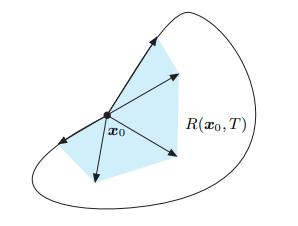
\includegraphics[width=\textwidth]{Images/image9.png}
                    \caption{Controllability: 
                     $R(x_0,T )$ is not a neighborhood of $x_0$.}
                    \label{fig:controllability}
                \end{minipage}
                \hfill               
                \begin{minipage}{0.3\textwidth}
                    \centering
                    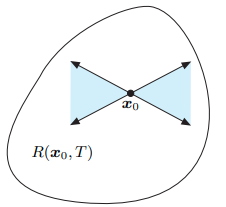
\includegraphics[width=0.5\linewidth]{Images/image10.png}
                    \caption{Small-Time Local Controllability: \\
                    In general, trajectories cannot progress from the point $x_0$ in all directions.}
                    \label{fig:small_time_controllability}
                \end{minipage}
                \hfill
                \begin{minipage}{0.3\textwidth}
                    \centering
                    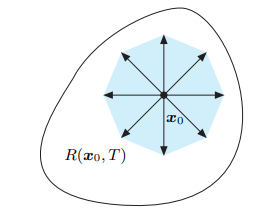
\includegraphics[width=0.5\linewidth]{Images/image11.png}
                    \caption{Omnidirectional Controllability: \\
                    The trajectories can progress starting from $x_0$ in all directions.}
                    \label{fig:omni_controllability}
                \end{minipage} \hfill
            \end{figure}
            The concept of controllability can be more easily applied to control-affine systems, by defining the \textit{Accessibility Distribution}:
            \begin{definition}
                \textbf{Accessibility Distribution}: Let:
                \begin{equation*}
                    \dot{x}=f(x)+\sum_{i=0}^{d}g_{i}(x)u_i
                \end{equation*}
                Be a control-affine system. Then, let the \textit{Accessibility Distribution} $\Delta_{A}$ be the distribution generated by the vector fields $f,g_i$ and all the Lie Brackets that can be generated by them. 
            \end{definition}
            Assuming that the vector fields are all $C^\infty$ \footnote{Meaning that they are continuously differentiable, for every order of derivation: $\frac{d^{(n)}}{dx^{(n)}}f$ is continuously differentiable, for all $n \in \mathbb{N}$.}, then if $\dim(\Delta_a)=n$ for all times, the accessible set $R(x_0,T)$ has a non-empty interior: the system is always accessible. This is summarized by the theorem:
            \begin{theorem}\label{Accessibility_rank_condition}
                \textbf{Accessibility Rank Condition}: A Control-Affine system:
                \begin{equation*}
                    \dot{x} = f(x)+\sum_{i=1}^{d}g_i(x)u_i
                \end{equation*}
                Where $f,g_i$, for $i \in \{1,\dots,d\}$ are $C^\infty$, is accessible from $x_0$ if the following \textit{accessibility rank condition} is satisfied:
                \begin{equation}\label{acc_rank_cond}
                    \dim(\Delta_a(x_0))=n
                \end{equation}
                If the condition is satisfied for all $x \in U \subseteq\mathbb{R}^{n}$, then the system is controllable on $U$.
            \end{theorem}
            Geometrically speaking, this statement implies that the system can move along any direction on the tangent hyperplane to the system's dynamics manifold at the point $x\in U$.	  \newpage
\chapter{Wheeled Robots}
\section{Introduction}
\textit{Wheeled Robots} are the first and most basic form of mobile robots. Their mathematical description is easy compared to other types of mobile robots and relies heavily on the introduction of \textit{kinematic models}, in contrast to dynamic ones. A \textit{kinematic model} is a description of a robot's configuration, which doesn't take into account dynamical effects. \\
Wheeled robots cannot, generally speaking, move freely in the environment due to their structure; for example, it is easy to notice that a car cannot arbitrarily translate along the line joining the center of the front (or back) wheels, at any time. These constraints have to be included into the kinematic model of the robot.
\section{Motion Constraints}
Let $q \in \mathbb{R}^{n}$ be the vector of the robot's generalised coordinates; many types of constraints can be applied to the robot's model:
\begin{itemize}
    \item \textit{Unilateral Constraints}: expressed as inequalities. 
    \item \textit{Bilateral Constraints}: expressed as equalities.
    \item \textit{Rheonomic Constraints}: time dependent constraints.
    \item \textit{Scleronomic Constraints}: time independent constraints.
\end{itemize}
There are also \textit{kinematic constraints}, which are of great importance.
\begin{definition}\label{kin_constrs_def}
    \textbf{Kinematic Constraints}: Let $a_i^T:\mathbb{R}^{n}\rightarrow\mathbb{R}^{n^*}$ be linearly independent smooth co-vector fields. Constraints in the form:
    \begin{equation}\label{kine_constrs}
        a_i(q,\dot{q})=0, \text{ } i\in \{1,\dots,k\}, \textbf{ }k<n
    \end{equation}
    Are called \textit{kinematic constraints}, which reduce the set of generalised velocities that can be attained at each model-configuration.
\end{definition}
Kinematic constraints can be expressed into \textit{Pfaffian Form}:
\begin{equation}\label{Pfaffian_form}
    a_i^T(q)\dot{q}=0, \textbf{ } i \in \{1,\dots,k\}, \textbf{ }k<n
\end{equation}
Or equivalently:
\begin{equation}\label{pfaffian_matrix}
    A^T(q)\dot{q}=0
\end{equation}
Where the matrix $A^T(q)$ is the \textit{Pfaffian Matrix}. \\
Another set of constraints of great importance is the set of
\textit{holonomic constraints} or \textit{integrable constraints}.
\begin{definition}\label{holo_constr_def}
    \textbf{Integrable Constraints}: Let $h:\mathbb{R}^{n} \rightarrow \mathbb{R}$ and $h_i \in C^\infty$, for $i \in \{1,\dots,k\}$. Constraints of the form:
    \begin{equation}\label{holo_constrs}
        h_i(q)=0, \text{ }i\in \{1,\dots,k\}, \text{ } k<n
    \end{equation}
    Are called \textit{holonomic} or \textit{integrable} constraints. Their effect is to \textit{reduce the space of admissible model-configurations} to a subset $U \subset \mathbb{R}^{n}$ of dimension $n-k$.
\end{definition}
Each holonomic constraint can be expressed into Pfaffian form (but the converse is not true):
\begin{equation*}
    h_i(q)=0 \rightarrow \frac{d}{dt}h_i(q)=\frac{\partial h_i(q)}{\partial q} \dot{q}=0
\end{equation*}
If a Pfaffian constraint is not integrable, it is called \textit{nonholonomic}. A system is nonholonomic if it has at least one nonholonomic constraint.\\
The last statement leads naturally to the question of how can it be determined if the system:
\[A^T(q)\dot{q}=0\]
Is integrable or not; to answer this question, it is first necessary to investigate the controllability characteristic of the robotic system: a \textit{kinematic model} is needed. \\
Suppose to have a mechanical system subject to the Pfaffian constraints:
\begin{equation*}
    A^T(q)\dot{q}=0, \quad A^T \in \mathbb{R}^{k\times n}, \quad q,\dot{q} \in \mathbb{R}^n
\end{equation*}
The objective is to understand along which of the $n-k=m$ directions the system can move. Since the constraints have to be always satisfied, a distribution can be constructed out of the nullspace of $A^T$:
\begin{equation*}
    \Delta = \text{span}\left\{g_j(q)\in \mathbb{R}^{n}: A^T(q)g_j(q)=0, \textbf{ } j \in \{1,\dots,m\}\right\}
\end{equation*}
Then, if $q \in \Delta$:
\begin{equation*}
    \dot{q}=\sum_{j=1}^{m}g_j(q)u_j=G(q)u \in \Delta
\end{equation*}
The expression:
\begin{equation}\label{kin_model}
    \dot{q}=G(q)u
\end{equation}
Is the \textit{kinematic model} of the mechanical system. Two points are to be noticed:
\begin{itemize}
    \item The kinematic model \textit{is not} unique. 
    \item The kinematic model is a driftless affine control system.
\end{itemize}
Being built directly from the set of constraints, the kinematic model contains embedded information about the constraints themselves; in particular, the controllability of the system influences the nature of the constraints.
\begin{itemize}
    \item If $\dot{q}=G(q)u$ is controllable, the following are equivalent: \begin{itemize}
        \item The system is subjected only to nonholonomic constraints.
        \item The accessibility rank condition of Theorem (\ref{Accessibility_rank_condition}) is met.
        \item $A^T(q)\dot{q}=0$ is not integrable.
    \end{itemize}
    \item If $\dot{q}=G(q)u$ is not controllable, the following are equivalent:
    \begin{itemize}
        \item The system has some holonomic constraints.
        \item $m<\dim(\Delta_a)<n$ and $A^T(q)\dot{q}=0$ have only partially integrable constraints. However, the system is still nonholonomic.
    \end{itemize}
    Or:
    \begin{itemize}
        \item The system is subjected to holonomic constraints only.
        \item if $m=\dim(\Delta_a)$, then $A^T(q)\dot{q}=0$ has only integrable constraints, where $A^{T}$ has the vectors $\{g_1(q),\dots,g_m(q)\}$ as its columns.
    \end{itemize}
    \section{Equations of motion with nonholonomic constraints}
    Suppose to have a system subjected to at least one nonholonomic constraint. In that case, the mathematical model is modified to include the constraints:
    \begin{gather}\label{nonholo_model}
        M(q)\ddot{q}+h(q,\dot{q})=B(q)\tau+A(q)\lambda \\
        A^{T}(q)\dot{q}=0
    \end{gather}
    Making use of the \textit{Lagrange Multipliers} $\lambda\in\mathbb{R}^{k}$; the term $A(q)\lambda$ maps the reaction forces to the generalised coordinates space. Solving this system is going to give the dynamics and Lagrange Multipliers. Starting from:
    \begin{gather*}
        \frac{d}{dt}\left(A^T(q)\dot{q}\right)=0\rightarrow \\
        A^{T}(q)\ddot{q}+\dot{A}^{T}(q)\dot{q}=0
    \end{gather*}
    Rewriting the generalised acceleration as:
    \begin{gather*}
        \ddot{q}=M^{-1}\left( B\tau+A\lambda-h \right)
    \end{gather*}
    Where the dependencies have been dropped for space. Substituting back into the Pfaffian constraints' derivative:
    \begin{gather*}
        A^{T}M^{-1}\left(B\tau+A\lambda-h\right)+\dot{A}^{T}\dot{q}=0 \rightarrow \\
        A^{T}M^{-1}A\lambda=-A^{T}M^{-1}A\left(B\tau-h\right)-\dot{A}^{T}\dot{q}
    \end{gather*}
    If the $k$ Pfaffian constraints are independent, then $A^{T}M^{-1}A$ is invertible and the Lagrange Multipliers can be computed:
    \begin{equation}\label{lagrange_mult_comp}
        \lambda=\left[A^{T}M^{-1}A\right]^{-1}\left[-A^{T}M^{-1}\left(B\tau-h\right)-\dot{A}^{T}\dot{q}\right]
    \end{equation}
    However, sometimes it is also useful to not solve directly for the multipliers; to this end, both sides of the dynamic model have to be multiplied by the kinematic model matrix $G(q)$:
    \begin{gather*}
        G^{T}(q)M(q)\ddot{q}+G^{T}(q)h(q,\dot{q})=G^{T}(q)B(q)\tau+G^{T}(q)A(q)\lambda
    \end{gather*}
    Since $G(q)=[g_1(q)\dots g_n(q)]$ and $g_i(q)\in Null(A)$ for all $i \in \{1,\dots,d\}$ and taking into account the kinematic model eq: \ref{kin_model}:     
    \begin{gather*}
        \ddot{q}=\dot{G}(q,\dot{q})u+G(q)\dot{u}\rightarrow\\
        [G^{T}(q)M(q)]\ddot{q}=[G^{T}(q)M(q)]\dot{G}(q)u+[G^{T}(q)M(q)]G(q)\dot{u}
    \end{gather*}
    From which the following can be obtained:
    \begin{gather*}
        \left[G^{T}(q)M(q)G(q)\right]\dot{u}+\left[G^{T}(q)M(q)\dot{G}(q)u+G^{T}(q)h(q,\dot{q})\right]=G^{T}(q)B(q)\tau \rightarrow \\
        \bar{M}(q)\dot{u}=m(q,\dot{q},u)=G^{T}(q)B(q)\tau
    \end{gather*}
    By manipulating this equation, the system of $m+n$ equations is obtained:
    \begin{gather*}
        \begin{cases}
            \dot{u}=-\bar{M}^{-1}(q)m(q,\dot{q},u)+\bar{M}^{-1}(q)G^{T}(q)B(q)\tau \\
            \dot{q}=G(q)u
        \end{cases}
    \end{gather*}
    This system is feedback linearizable and assuming that $G^{T}(q)B(q)$ is full-rank, the input:
    \begin{equation*}
        \tau=\left[G^{T}B\right]^{-1}\left[\bar{M}a+m\right]
    \end{equation*}
    Can be used to decouple and linearize the system, giving as a result:
    \begin{equation*}
        \begin{cases}
            \dot{u}=a \text{, $m$ integrators on the input channel}\\
            \dot{q}=G(q)u \text{, kinematic model}
        \end{cases}
    \end{equation*}
    Finally, the two equations can be united into a new type of kinematic model called \textit{Second-Order Kinematic Model}:
    \begin{equation}\label{sec_ord_kin_mod}
        \dot{\bar{x}}=
        \begin{bmatrix}
            G(q)u \\
            0
        \end{bmatrix}
        +
        \begin{bmatrix}
            0 \\
            I_{m}
        \end{bmatrix}
        a
    \end{equation}
\end{itemize}
\subsection{Examples: Kinematic Models}
\subsubsection{Disk rolling on a plane, Unicycle and Differential Drive Robot}
By introducing the generalised coordinates $q=\begin{bmatrix}x & y & \theta\end{bmatrix}$, the cartesian velocities of the contact point with ground are easily found to be:
\begin{equation*}
    \begin{cases}
        \dot{x}=\rho \dot{\phi} \cos(\theta) \\
        \dot{y}=\rho \dot{\phi} \sin(\theta) 
    \end{cases}
\end{equation*}
This then leads to:
\begin{gather*}
    \begin{cases}
        \dot{x}\sin(\theta)=\rho \dot{\phi} \cos(\theta) \sin(\theta) \\
        \dot{y} \cos(\theta) = \rho \dot{\phi} \cos(\theta) \sin(\theta) 
    \end{cases}\rightarrow \\
    \dot{x}\sin(\theta)-\dot{y}\cos(\theta)=0
\end{gather*}
This last equation represents the \textit{pure rolling constraint}. Since the coin cannot slip, it has to have zero velocity along the axis of the sagittal plane, giving us the constraint in Pfaffian form:
\begin{equation*}
    \begin{bmatrix}
        \sin(\theta) & -\cos(\theta) & 0
    \end{bmatrix}
    \begin{bmatrix}
        \dot{x} \\ \dot{y} \\ \dot{\theta}
    \end{bmatrix}
    =0
\end{equation*}
Since this constraint has dimension $k=1$ and the state space $n=3$, Rank$(G)=2=n-k=m$. By inspection, another vector linearly independent from the one in the rolling constraint is $g_2=\begin{bmatrix} 0 & 0 & 1 \end{bmatrix}$, giving:
\begin{equation*}
    G(q)=
    \begin{bmatrix}
        0 & \cos(\theta) \\
        0 & \sin(\theta) \\
        1 & 0
    \end{bmatrix}
\end{equation*}
To understand if the constraint is holonomic, the Lie Bracket $[g_1,g_2]$ is computed:
\begin{gather*}
    [g_1,g_2]
    =
    \begin{bmatrix}
        0 & 0 & -\sin(\theta) \\
        0 & 0 & \cos(\theta) \\
        0 & 0 & 0
    \end{bmatrix}
    \begin{bmatrix}
        0 \\ 0 \\ 1
    \end{bmatrix}
    -
    O\frac{\partial g_1}{\partial x}=\\
    \begin{bmatrix}
        -\sin(\theta) \\
        \cos(\theta) \\
        0
    \end{bmatrix}
\end{gather*}
Putting all these vectors into a matrix and computing its determinant:
\begin{gather*}
    F=
    \begin{bmatrix}
        0 & \cos(\theta) & -\sin(\theta) \\
        0 & \sin(\theta) & \cos(\theta) \\
        1 & 0 & 0
    \end{bmatrix} \\
    \det(F)=1, \textbf{ } \forall q \in \mathbb{R}^3
\end{gather*}
So that the system is controllable and completely nonholonomic: the constraint is not integrable.
\begin{figure}[htbp!]
    \begin{minipage}{0.5\textwidth}
        \centering                  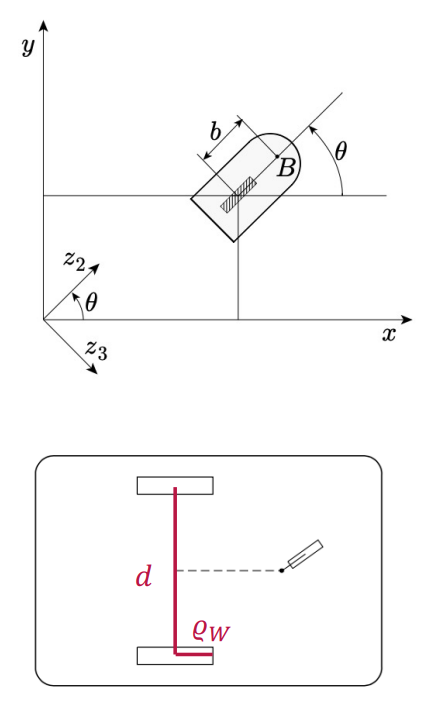
\includegraphics[width=0.5\linewidth]{Images/image13.png}
        \caption{Unicycle Robot and Differential Drive Robot.}
        \label{fig:uni_cycle}
    \end{minipage}
    \hfill
    \begin{minipage}{0.5\textwidth}
        A \textit{unicycle} robot is generally composed of a single wheel and a rigid chassis; however, due to its inherent instability, there are robots which are kinematically equivalent to a unicycle, but have more than one wheel, granting static stability, such as the \textit{Differential Drive Robot}. Both are kinematically equivalent to the disc rolling on a plane.\\
        The unicycle inputs are its heading velocity $v$ and steering velocity $\omega$. Usually, these are mapped into wheel velocities (in the case of the second robot) as:
        \begin{gather*}
            v = \frac{\omega_{R}+\omega_{L}}{2}\rho_{W} \text{, } \omega=\frac{\omega_{R}-\omega_{L}}{d}\rho_{W} \\
            \omega_{R}=\frac{2v+\omega d}{2\rho_{W}} \text{, } \omega_{L}=\frac{2v-\omega d}{2\rho_{W}}
        \end{gather*}
    \end{minipage}
\end{figure}
\subsubsection{Bycicle Robot}
\begin{figure}[htbp!]
    \begin{minipage}{0.6\textwidth}
        \centering                  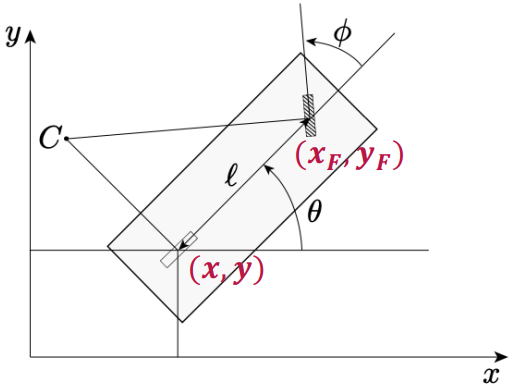
\includegraphics[width=0.6\linewidth]{Images/image15.png}
        \caption{Bycicle Robot.}
    \end{minipage}
    \hfill
    \begin{minipage}{0.4\textwidth}
        The \textit{Bycicle Robot} is kinematically equivalent to a car-like robot and is often used as a simplified model for it. The generalised coordinates are:
        \[q= \begin{bmatrix}
            x & y & \theta & \phi
        \end{bmatrix}\]
    \end{minipage}
\end{figure}
Each wheel has a pure rolling constraint:
\begin{gather*}
    \begin{cases}
        \dot{x}\sin(\theta)-\dot{y}\cos(\theta)=0 \\
        \dot{x}_{F}\sin(\theta+\phi) - \dot{y}_{F}\cos(\theta+\phi)=0
    \end{cases}
\end{gather*}
These can be brought into Pfaffian form by expressing the coordinates of the front wheel with respect to the rear wheel and substituting back into the previous equations:
\begin{equation*}
    \begin{cases}
        x_F=x+l\cos(\theta) \\
        y_F=y+l\sin(\theta)
    \end{cases} \rightarrow
    \begin{cases}
        \dot{x}\sin(\theta)-\dot{y}\cos(\theta)=0 \\
        \dot{x}\sin(\theta+\phi) - \dot{y}\cos(\theta+\phi)-l\dot{\theta}\cos(\phi)=0
    \end{cases}
\end{equation*}
Since the number of constraints is $k=2$ and the state space is four-dimensional, the Rank of $G$ has to be $m=n-k=2$; the Pfaffian Matrix is given as:
\begin{equation*}
    A=
    \begin{bmatrix}
        \sin(\theta) & - \cos(\theta) & 0 & 0 \\
        \sin(\theta+\phi) & \cos(\theta+\phi) & -l\cos(\phi) & 0
    \end{bmatrix}
\end{equation*}
Two vectors spanning its Null are:
\begin{equation*}
    g_1=
    \begin{bmatrix}
        \cos(\theta)\cos(\phi)\\
        \sin(\theta)\cos(\phi)\\
        \sin(\phi/l)\\
        0
    \end{bmatrix}, 
    g_2 =
    \begin{bmatrix}
        0 \\ 0 \\ 0 \\ 1
    \end{bmatrix}
\end{equation*}
Then the kinematic model is:
\begin{equation*}
    \dot{q} =
    \begin{bmatrix}
        \cos(\theta)\cos(\phi)\\
        \sin(\theta)\cos(\phi)\\
        \sin(\phi/l)\\
        0
    \end{bmatrix}
    v+
    \begin{bmatrix}
        0 \\ 0 \\ 0 \\ 1
    \end{bmatrix}
    \omega
\end{equation*}
Let's check for the controllability by making use of the accessibility condition eq: \ref{Accessibility_rank_condition}:
\begin{gather*}
    \Delta_{a}(q)=span\left\{g_1,g_2,[g_1,g_2],[g_1,[g_1,g_2]]\right\} \\
    g_3=
    \begin{bmatrix}
        \cos(\theta)\sin(\phi)\\
        \sin(\theta)\sin(\phi)\\
        -\cos(\phi/l) \\
        0
    \end{bmatrix}, 
    g_4=
    \begin{bmatrix}
        -\sin(\theta/l)\\
        \cos(\theta/l) \\
        0\\
        0
    \end{bmatrix}
\end{gather*}
Since the condition is satisfied, $Dim(\Delta_a)=4$, the system is controllable and completely non-holonomic.
\subsubsection{Dynamic Model of the unicycle}
To obtain the dynamic model of a unicycle the first step is to define the model's parameters:
\begin{itemize}
    \item $m$ is the robot's mass.
    \item $J$ is the robot's moment of inertia around its vertical axis.
    \item $\tau_1$ is the driving torque.
    \item $\tau_2$ is the steering torque.
\end{itemize}
Then, writing the model as in eq: \ref{nonholo_model}:
\begin{gather*}
    \begin{cases}
        M(q)\ddot{q}+h(q,\dot{q})=B(q)\tau+a(q)\lambda \\
        a^{T}(q)\dot{q}=0
    \end{cases}
    \rightarrow \\
    \begin{cases}
        \begin{bmatrix}
            m & 0 & 0 \\
            0 & m & 0 \\
            0 & 0 & m
        \end{bmatrix}
        \ddot{q} =
        \begin{bmatrix}
            \cos(\theta) & 0 \\
            \sin(\theta) & 0 \\
            0 & 1                                            
        \end{bmatrix}
        \tau + 
        \begin{bmatrix}
            \sin(\theta) \\
            -\cos(\theta)\\
            0
        \end{bmatrix} \lambda\\
        \begin{bmatrix}
            \sin(\theta) & -\cos(\theta) & 0
        \end{bmatrix}
        \dot{q}=0
    \end{cases}
\end{gather*}
By the same steps seen in the previous section, the following second order kinematic model is obtained:
\begin{gather*}
    \begin{cases}
        \dot{u} =
        \begin{bmatrix}
            \dot{v} \\
            \dot{\omega}
        \end{bmatrix}
        =
        \begin{bmatrix}
            \frac{1}{m} & 0 \\
            0 & \frac{1}{J}
        \end{bmatrix}
        \tau \\
        \dot{q} = 
        \begin{bmatrix}
            \cos(\theta) & 0\\
            \sin(\theta) & 0\\
            0 & 1
        \end{bmatrix}u
    \end{cases} \rightarrow \\
    \begin{cases}
        \dot{u} =
        \begin{bmatrix}
            \dot{v} \\
            \dot{\omega}
        \end{bmatrix}
        =
        \begin{bmatrix}
            \frac{1}{m} & 0 \\
            0 & \frac{1}{J}
        \end{bmatrix}
        \left\{\left[G^{T}(q)B(q)\right]^{-1}\left[\bar{M}(q)a+m(q,\dot{q})\right]\right\} \\
        \dot{q} = 
        \begin{bmatrix}
            \cos(\theta) & 0\\
            \sin(\theta) & 0\\
            0 & 1
        \end{bmatrix}u
    \end{cases}\rightarrow \\
    \begin{cases}
        \dot{u} =
        \begin{bmatrix}
            \dot{v} \\
            \dot{\omega}
        \end{bmatrix}
        =
        \begin{bmatrix}
            \frac{1}{m} & 0 \\
            0 & \frac{1}{J}
        \end{bmatrix}
        \begin{bmatrix}
            m & 0\\
            0 & J
        \end{bmatrix}a \\
        \dot{q} = 
        \begin{bmatrix}
            \cos(\theta) & 0\\
            \sin(\theta) & 0\\
            0 & 1
        \end{bmatrix}u
    \end{cases} \rightarrow \\
    \begin{cases}
        \dot{u} = a \\
        \dot{q} =
        \begin{bmatrix}
            \cos(\theta) & 0\\
            \sin(\theta) & 0\\
            0 & 1
        \end{bmatrix}u
    \end{cases}
\end{gather*}
\section{Low-level Planning}
A mobile robot needs to be able to plan its movements in the environment; this is really a two-fold problem, since a movement implies a \textit{path} to follow and a \textit{time law} (i.e, velocity and acceleration) with which the path has to be traveled. Formally speaking:
\begin{definition}\label{trajecotry_planning_problem}
    (\textit{Trajectory Planning Problem}): The problem of \textit{Trajectory Planning} is based on constructing both a \textit{path} and a \textit{time law}, i.e., a \textit{trajectory} $q(t)$ for $t\in [t_0, t_f]$, leading the robot from $q(t_i)=q_0$ to $q(t_f)=q_f$ in the absence of obstacles and subject to nonholonomic constraints.
\end{definition}
A \textit{Geometric Path} is a parametric function $f(s)$, which describes only the geometric aspect of the trajectory: it does not deliver any information about the velocity of travel. Similarly, a \textit{Time Law} is a strictly monotonic function $s(t)$ such that $s(t_i)=s_i,s(t_f)=s_f,\dot{s}(t)>0$ for all $t \in [t_0,t_f]$ (i.e., the curve is \textit{regular}). It is often the case that the parameter $s$ is the \textit{curvilinear abscissa} or \textit{arclength}. The division of the two descriptions then leads to a mathematical formulation of the trajectory as:
\begin{equation*}
    \dot{q}(t)=\frac{dq}{ds}\frac{ds}{dt}=q'(s)\dot{s}
\end{equation*}
As is known from Calculus, the vector $q'=t$ is the tangent vector to the path, with unit-norm in the case of $s$ as arclength. Since the robot has to comply with the kinematic constraints, this separation is carried out also in the Pfaffian form eq: \ref{Pfaffian_form}:
\begin{equation*}
    A^T(q)\dot{q}(q)=A^T(q)q'(s)\dot{s}(t)=0
\end{equation*}
Since $\dot{s}>0$ for all times:
\begin{equation*}
    A^T(q)q'(s)=0
\end{equation*}
Similarly, as to how the admissible velocities for the kinematic model were retrieved, a \textit{Geometric Admissible Path} can now be generated directly from the constraints:
\begin{equation*}
    q'(s)=G(q)\tilde{u}(s)
\end{equation*}
With $u(t)=\tilde{u}(s)\dot{s}(t)$ and $\tilde{u}(s)$ are called \textit{geometric inputs}. Once these are defined, the path of the robot in the model-configuration space is uniquely determined.
\subsection{Example: Unicycle}
The pure rolling constraint is given by:
\begin{equation}\label{Pure_rolling}
    \begin{bmatrix}
        \sin(\theta) & \cos(\theta) & 0
    \end{bmatrix}
    \begin{bmatrix}
        \dot{x} \\ \dot{y} \\ \dot{z}
    \end{bmatrix}=0
\end{equation}
Expressing it as a geometrical constraint (neglecting any non-geometric information about the trajectory):
\begin{equation}
    \begin{bmatrix}
        \sin(\theta) & \cos(\theta) & 0
    \end{bmatrix}
    \begin{bmatrix}
        x' \\ y' \\ z'
    \end{bmatrix}=0
\end{equation}
Since the kinematic model for the unicycle is known, the admissible path are directly given by:
\begin{gather}\label{geo_uni_mod}
    \begin{bmatrix}
        x' \\ y' \\ z'
    \end{bmatrix}=
    \begin{bmatrix}
        0 \\ 0 \\ 1
    \end{bmatrix}\tilde{\omega} +
    \begin{bmatrix}
        \cos(\theta) \\ \sin(\theta) \\ 0
    \end{bmatrix} \tilde{v}
\end{gather}
\subsection{Path Planning and Differential Flatness for the unicycle}
Path planning, in the case of a unicycle, is relatively simple since it is a differentially flat system with $x$ and $y$ as flat outputs. As is known from Control Theory, for a flat system it is possible to compute the exact feedforward control necessary to follow a specified reference variable by input-to-output linearizing the system. \\
Taking into account the geometric unycicle model in eq: \ref{geo_uni_mod}, the pair $(x,y)$ is a flat output and it is possible to derive the following control inputs:
\begin{gather*}
    \begin{cases}
        \theta(s)=atan2(y'(s),x'(s))+k\pi, k=\{0,1\} \\
        \tilde{v}(s)=\pm \sqrt{x'(s)^2+y'(s)^2}\\
        \tilde{\omega}(s)=\frac{y"(s)x'(s)-x"(s)y'(s)}{x'(s)^2+y'(s)^2}
    \end{cases}
\end{gather*}
Where $k=0$ for forward motion, $k=1$ for backward motion. Notice that $x'=y'=0$ is not allowed, which means that the path must be without cusps and never shrinks to a point. \\
Path planning can be carried out with many strategies, assuming to know the initial $q_0$ and final configuration $q_f$ of the robot. 
\subsubsection{Planning via Cartesian Polynomials}
The most natural strategy is to employ Cartesian Polynomials; these should be at least of third degree to have a well-behaved geometric path. Consider then the following cubic polynomials:
\begin{gather*}
    \begin{cases}
        x(s)=s^3x_f-(s-1)^3x_i+\alpha_xs^2(s-1)+\beta_xs(s-1)^2 \\
        y(s)=s^3y_f-(s-1)^3y_i+\alpha_ys^2(s-1)+\beta_ys(s-1)^2
    \end{cases}
\end{gather*}
With $k_i\neq0,k_f\neq0,k_{i}k_{f}>0$ for forward motion. Assuming to know both the initial and final configurations, all the coefficients can be computed; for example, suppose to have a forward motion with $k_i=k_f=k>0$ as:
\begin{gather*}
    \alpha_x=k\cdot \cos(\theta_f)-3x_f \\
    \alpha_y=k\cdot \sin(\theta_f)-3y_f \\
    \beta_x=k\cdot \cos(\theta_i)+3x_i \\
    \beta_y=k\cdot \sin(\theta_i)+3y_i
\end{gather*}
Once an admissible path $q(s)$ has been chosen, a time law $s(t)$ can be formulated. However, it can happen that the computed time law is not feasible (it could imply velocities which exceed the maximum allowed ones), so that a \textit{Scaling} technique has to be used. An example of such a technique is \textit{Uniform Scaling}. Recalling that $\omega(t)=\tilde{\omega}(s)\dot{s}(t)$, $v(t)=\tilde{v}(s)\dot{s}(t)$, assume to redefine the time parameter as $\tau=t/(t_f-t_i)=t/T$:
\begin{gather*}
    v(t)=\tilde{v}(s)\frac{ds}{dt}=\tilde{v}(s)\left[\frac{1}{T}\frac{ds}{d\tau}\right] \\
    \omega(t)=\tilde{\omega}(s)\frac{ds}{dt}=\tilde{\omega}(s)\left[\frac{1}{T}\frac{ds}{d\tau}\right]
\end{gather*}
So that by increasing $T$ the trajectories are scaled uniformly.
\subsection{Optimal Trajectories}
As is known, the \textit{Pontryagin's Minimum Principle}  is used within \textit{Optimal Control Theory} to find the best possible control for taking the system from one state to another, in the presence of state and control constraints. 
\begin{definition}\label{Pontryagin_Min_Principle}
    (\textit{Pontryagin's Minimum Principle}): Consider an $n$-dimensional dynamic system, with state variable $x \in \mathbb{R}^{n}$, control variable $u\in\mathcal{U}$ ($\mathcal{U}$ is the set of admissible controls). The evolution of the system is determined by the state and the control, according to the differential equation:
    \begin{equation*}
        \dot{x}=f(x,u), \; x(0)=x_0, \; u(t)\in\mathcal{U}, \; t\in[0, T]
    \end{equation*}
    The control trajectory is chosen according to a \textit{Objective Functional}:
    \begin{equation*}
        J=\Psi(x(T))+\int_{0}^{T}{L(x(t),u(t))dt} 
    \end{equation*}
    Where $L(\cdot,\cdot)$ is the \textit{Cost-to-go} and $\Psi(\cdot)$ is the \textit{Final Cost}. The system's constraints are introduced by making use of the Lagrange Multipliers $\lambda(t)$ and the Hamiltonian:
    \begin{equation*}
        H(x(t),u(t),\lambda(t),t)=\lambda^{T}(t)\cdot f(x(t),u(t))+L(x(t),u(t))
    \end{equation*}                                    
    Defined for all $t\in[0,T]$. Then, Pontryagin's minimum principle states that:
    \begin{itemize}
        \item  The optimal state trajectory $x^*$, optimal $u^*$, and corresponding Lagrange Multiplier vector $\lambda^*$ must minimize the Hamiltonian $H$, such that:
        \begin{equation}\label{Hamiltonian_Minimization}
            H(x^*(t),u^*(t),\lambda^*(t),t)\leq H(x(t),u,\lambda(t),t)
        \end{equation}
        For all $t\in[0,T]$ and $u \in \mathcal{U}$. 
        \item If $x(T)$ is fixed, the Lagrange Multipliers must satisfy:
        \begin{gather}\label{fixed_state_lagrangian_mult}
            -\dot{\lambda}(t)=H_{x}(x^*(t),u^*(t),\lambda(t),t)=\lambda^{T}f_x(x^*,u^*)+L_{x}(x^*,u^*) \\
            \lambda^{T}(T)=\Psi_{x}(x(T))
        \end{gather}
        \item If $x(T)$ is not fixed, then the Lagrange Multipliers must also satisfy:
        \begin{equation}\label{not_fixed_state_lagrangian_mult}
            \Psi_{T}(x(T))+H(T)=0
        \end{equation}
    \end{itemize}
    If the conditions are met, then an optimal state and control trajectory are found.
\end{definition}
This principle can be used to plan trajectories. 
\subsubsection{Minimum-Time Trajectories}
\begin{figure}[htbp!]
    \begin{minipage}{0.4\textwidth}
        \centering
        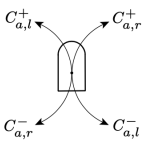
\includegraphics[width=0.5\linewidth]{Images/image17.png}
        \caption{Reeds-Shepp Line Arcs.}
        \label{fig:Reeds_Shepp}
    \end{minipage}\hfill
    \begin{minipage}{0.4\textwidth}
        \centering
        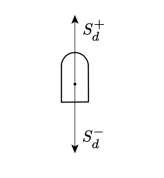
\includegraphics[width=0.5\linewidth]{Images/image18.png}
        \caption{Reeds-Shepp Line Segments.}
    \end{minipage}
\end{figure}
Consider the problem of moving a unicycle from an initial configuration $q_i$ to $q_f$. Then, applying Pontryagin's Minimum Principle, it is possible to find a sufficient family of candidate trajectories. This family, called \textit{Reed-Shepp Curves}, consists of trajectories obtained by concatenating elementary arcs of two types:
\begin{itemize}
    \item Line segments of variable length covered with velocities $v(t)=\pm v_{max}$ and $\omega(t)=0$.
    \item Arc of circles of variable length covered with velocities $v(t)=\pm v_{max}$ and $\omega(t)= \pm \omega_{max}$.
\end{itemize}
The trajectories are grouped into 9 sets.
\begin{figure}[htbp!]
    \begin{minipage}{0.7\textwidth}
        \centering
        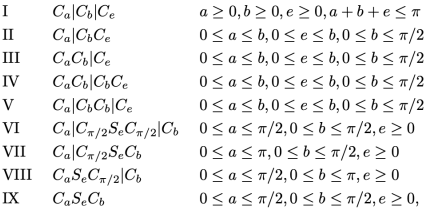
\includegraphics[width=0.7\linewidth]{Images/image19.png}
        \caption{Reed-Shepps Curves grouped. \\Each '$|$' is an inversion of motion on the path.}
        \label{fig:Reed_Shepps_Curves}
    \end{minipage}\hfill
    \begin{minipage}{0.3\textwidth}
        Each group contains trajectories consisting of a sequence of no more than $5$ elementary arcs/segments and produces a finite number of sequences; for example, for Group $IX$: 
    \end{minipage} 
\end{figure}\\
All-in-all, there are $48$ different sequences, which are to be searched before finding the optimal one for the task at hand. An algorithm for such a search would look like:
\begin{itemize}
    \item Determine all trajectories feasible to link $q_i$ to $q_f$.
    \item Compute $J=t_i-t_f$ along the feasible trajectories.
    \item Chose the one which returns the minimum cost.
\end{itemize}
\begin{figure}[h!]
    \centering
    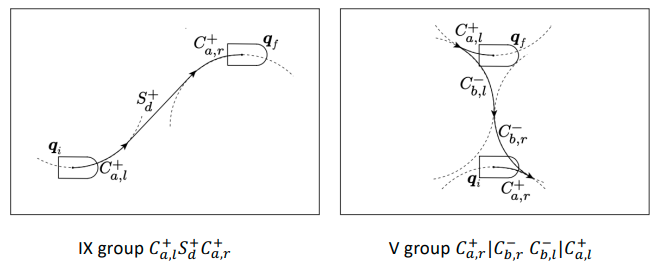
\includegraphics[width=0.8\linewidth]{Images/image21.png}
    \caption{Examples of paths using Reeds-Shepp Curves.}
\end{figure}
\section{High-Level Planning}
Up until now it has been assumed that no kinematic constraints were imposed on the robot; however, it has already been highlighted how an unicycle cannot move instantaneously in any arbitrary direction. A more general approach to Motion Planning consists in the use of motion primitives that are a finite set of admissible local paths in $\mathcal{C}$, each one produced by a given choice of the velocity inputs of the kinematic model. This is a \textit{High-level, Model-Based} problem. \\
There are two subproblems which constitute the \textit{High-Level Motion Planning} problem:
\begin{itemize}
    \item \textit{Tracking} a trajectory.
    \item \textit{Regulating} a configuration.
\end{itemize}
Here, only the case of a unicycle will be addressed, although there is not much difference, at least in the concepts, with other wheeled robots. 
\subsection{Unicycle Trajectory Tracking}
\begin{figure}[htbp!]
    \begin{minipage}{0.6\textwidth}
        \centering
        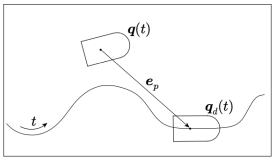
\includegraphics[width=0.6\linewidth]{Images/image24.png}
        \caption{Unicycle trajectory \\ tracking problem.}
        \label{fig:uni_traj_track}
    \end{minipage}\hfill
    \begin{minipage}{0.4\textwidth}
        A unicycle is a flat system. This enables the Motion Planner to compute the necessary inputs to the robot by specifying first the desired trajectory; this ensures compatibility between the prescribed trajectory and the robot's kinematic, since the control inputs are computed via the kinematic model (or dynamic model). 
    \end{minipage} 
\end{figure}
In the specific instance of the unicycle:
\begin{gather*}
    \theta_d(t)=atan2(\dot{y}(t),\dot{x}(t))+k\pi, \text{ }k\in\{0,1\} \\
    v_d(t)= \pm \sqrt{\dot{x}^2(t)+\dot{y}^2(t)}\\
    \omega_d(t)=\frac{\ddot{y}(t)\dot{x}(t)-\ddot{x}(t)\dot{y}(t)}{\dot{x}^2(t)+\dot{y}^2(t)}
\end{gather*}
To obtain a controller, the configuration error has to be defined. The n\"{a}ive approach would be to just get the difference between desired and current configurations, however it is much more convenient to express the error rotated in the current heading direction:
\begin{equation}\label{uni_traj_track_rotated_error}
    e(t)=
    \begin{bmatrix}
        e_1(t)\\e_2(t)\\e_3(t)
    \end{bmatrix}
    \begin{bmatrix}
        \cos(\theta) & \sin(\theta) & 0 \\
        -\sin(\theta) & \cos(\theta) & 0 \\
        0 & 0 & 1
    \end{bmatrix}
    \begin{bmatrix}
        x_d(t)-x(t)\\y_d(t)-y(t)\\\theta_d(t)-\theta(t)
    \end{bmatrix}
\end{equation}
Which has the dynamics:
\begin{equation}\label{uni_traj_track_err_dyn}
    \dot{e}(t)=\dot{\theta}
    \begin{bmatrix}
        -\sin(\theta) & \cos(\theta) & 0 \\
        -\cos(\theta) & -\sin(\theta) & 0 \\
        0 & 0 & 0
    \end{bmatrix}
    \begin{bmatrix}
        x_d(t)-x(t)\\y_d(t)-y(t)\\\theta_d(t)-\theta(t)
    \end{bmatrix} +
    \begin{bmatrix}
        \cos(\theta) & \sin(\theta) & 0 \\
        -\sin(\theta) & \cos(\theta) & 0 \\
        0 & 0 & 1
    \end{bmatrix}
    \begin{bmatrix}
        \dot{x}_d(t)-\dot{x}(t)\\\dot{y}_d(t)-\dot{y}(t)\\ \dot{\theta}_d(t)-\dot{\theta}(t)
    \end{bmatrix}
\end{equation}
Since the unicycle's kinematic model is given by (dropping the time dependence for convenience):
\begin{gather}\label{uni_kinematic_model}
    \begin{cases}
        \dot{x}_d=v_d\cos(\theta_d) \\
        \dot{y}_d=v_d\sin(\theta_d) \\
        \dot{\theta}_d=\omega_d
    \end{cases}
\end{gather}
Back substitution into the error dynamics eq:\ref{uni_traj_track_err_dyn} yields:
\begin{equation}\label{uni_traj_track_full_err_dyn}
    \begin{cases}
        \dot{e}_1=v_d\cos(e_3)-v+e_2\omega \\
        \dot{e}_2=v_d\sin(e_3)-e_1\omega \\
        \dot{e}_3=\omega_d-\omega
    \end{cases}
\end{equation}
To simplify the dynamics, it is possible to design the following transformations, where $u_1,u_2$ are virtual inputs:
\begin{gather*}
    v=v_d\cos(e_3)-u_1\\
    \omega=\omega_d-u_2
\end{gather*}
To decompose the dynamics into a linear and a non-linear term:
\begin{equation}\label{uni_traj_dec_error}
    \dot{e}=
    \begin{bmatrix}
        0 & \omega_d & 0 \\
        -\omega_d & 0 & 0 \\
        0 & 0 & 0
    \end{bmatrix}
    e+
    \begin{bmatrix}
        0 \\ \sin(e_3) \\ 0
    \end{bmatrix} v_d +
    \begin{bmatrix}
        1 & -e_2 \\
        0 & e_1 \\
        0 & 1
    \end{bmatrix}
    \begin{bmatrix}
        u_1 \\ u_2
    \end{bmatrix}
\end{equation}
Notice that:
\begin{itemize}
    \item The first term is linear.
    \item The first and second terms are time-varying and depend only on the desired velocities, but not states nor inputs.
\end{itemize}
Since this is a flat nonlinear system, there are a few obvious control approaches: \textit{linearization}, \textit{nonlinear control} and \textit{I/O Linearization}.
\subsubsection{Unicycle Trajectory Tracking: Linearization}
For the error dynamics eq:\ref{uni_traj_dec_error} assume that:
\begin{itemize}
    \item $\sin(e_{3})\approx e_{3}$.
    \item $-e_{2}u_{1}=0$.
    \item $e_{1}u_{2}=0$.
\end{itemize}
So that the decoupled error dynamics becomes:
\begin{equation*}
    \dot{e}=
    \begin{bmatrix}
        0 & \omega_d & 0 \\
        -\omega_d & 0 & v_d \\
        0 & 0 & 0
    \end{bmatrix} e +
    \begin{bmatrix}
        1 & 0 \\
        0 & 0 \\
        0 & 1
    \end{bmatrix}
    \begin{bmatrix}
        u_1 \\ u_2
    \end{bmatrix}
\end{equation*}
Which is a \textit{time-varying linear system}. To control such a system, a time-varying state feedback is sufficient:
\begin{gather}\label{uni_lin_feedback}
    u_1(t)=-k_1e_1(t) \\
    u_2(t)=-k_2e_2(t)-k_3e_3(t)
\end{gather}
Where $k_1,k_3>0$. The closed-loop becomes:
\begin{equation*}
    \dot{e}=
    \begin{bmatrix}
        -k_1 & \omega_d & 0 \\
        -\omega_d & 0 & v_d \\
        0 & -k_2 & -k_3
    \end{bmatrix} e
\end{equation*}
With a characteristic polynomial:
\[p(\lambda)=\lambda(\lambda+k_1)(\lambda+k_3)+\omega_d^2(\lambda+k_3)+v_dk_2(\lambda+k_1)\]
By choosing the gains' values as:
\begin{itemize}
    \item $k_1=k_2=2\zeta a$, with $0<\zeta<1$, $a>0$.
    \item $k_2=(a^2-\omega_d)/(v_d)$.
\end{itemize}
The eigenvalues are assigned such that:
\begin{itemize}
    \item $\lambda_1=-2\zeta a<0$.
    \item $\lambda_{2,3}$ are complex conjugates with negative real part.
    \item $\omega_n=a$ and the system has damping equal to $\zeta$.
\end{itemize}
However, the system is time-varying and there are no assurances about asymptotic stability. The system is indeed AS if the kinematic inputs $v_d,\omega_d$ are constant, such as along Reeds-Shepp curves. The result is local due to the linearization and notice also that:
\begin{equation*}
    k_2 \rightarrow \infty \text{ if } v_d \rightarrow 0
\end{equation*}
So that only \textit{persistent} trajectories, i.e. $|v_d|>0$, can be followed with this method; as a consequence, motion inversion cannot be allowed.
\subsubsection{\textit{Almost} nonlinear control}
Regarding the control error dynamics eq:\ref{uni_traj_dec_error} assume:
\begin{itemize}
    \item $-e_2u_1=0$.
    \item $e_1u_2=0$.
\end{itemize}
Then, the dynamics becomes:
\begin{equation*}
    \dot{e}=
    \begin{bmatrix}
        0 & \omega_d & 0 \\
        -\omega_d & 0 & 0 \\
        0 & 0 & 0
    \end{bmatrix}e+
    \begin{bmatrix}
        0 \\ \sin(e_3) \\ 0
    \end{bmatrix}v_d +
    \begin{bmatrix}
        1 & -e_2 \\ 0 & e_1 \\ 0 & 1
    \end{bmatrix}
    \begin{bmatrix}
        u_1 \\ u_2
    \end{bmatrix}
\end{equation*}
Let us consider the following state feedback:
\begin{gather}\label{uni_traj_nonlinear_in}
    u_1(t)=-k_1(v_d(t),\omega_d(t))e_1(t) \\
    u_2(t)=-k_2v_d(t) \frac{\sin(e_3(t))}{e_3(t)}e_2(t)-k_3(v_d(t),\omega_d(t))e_3(t)
\end{gather}
With $k_1,k_3>0$ bounded positive functions and $k_2>0$. If $v_d,\omega_d$, with their time derivatives, are bounded and persistent then the origin of the error dynamics becomes asymptotically stable under the control inputs proposed. This is easily proven by a Lyapunov stability analysis:
\begin{gather*}
    V=\frac{k_2}{2}(e_1^2+e_2^2)+\frac{e_3^2}{2} \rightarrow \\
    \dot{V}=k_2\omega_de_2e_1-k_2k_1(v_d,\omega_d)e_1^2+\\
    +k_2v_de_w\sin e_3-k_2\omega_de_2e_1-k_2v_de_2\frac{\sin e_3}{e_3}e_2-k_e(v_d,\omega_d)e_3^2=\\
    =-k_2k_1(v_d,\omega_d)e_1^2-k_3(v_d,\omega_d)e_3^2\leq 0
\end{gather*}
By hypothesis. However, since this is a \textit{semi}-definite Lie derivative, asymptotically stability cannot be inferred by Lyapunov's Theorem; to address asymptotical stability, Barbalat's Lemma is applied:
\begin{itemize}
    \item It can be shown that $\ddot{V}$ is bounded, so that $\dot{V}$ is uniformly continuous.
    \item $V(t)$ has a finite limit as $t\rightarrow\infty$.
\end{itemize}
Then, it follows from Barbalat's Lemma that $\dot{V}\rightarrow0$ as $t\rightarrow\infty$; but by the definition of $V$, this implies that $e_1\rightarrow e_2\rightarrow0$; also, the following holds:
\begin{equation*}
    \lim_{t\rightarrow+\infty} {\left(v_d^2+\omega_d^2\right)e_2^2}=0
\end{equation*}
Under the assumption of persistent trajectories, it follows that also $e_2$ tends to $0$ as $t\rightarrow\infty$.
\subsubsection{Input-Output Linearization}
\begin{figure}[htbp!]
    \begin{minipage}{0.6\textwidth}
        \centering
        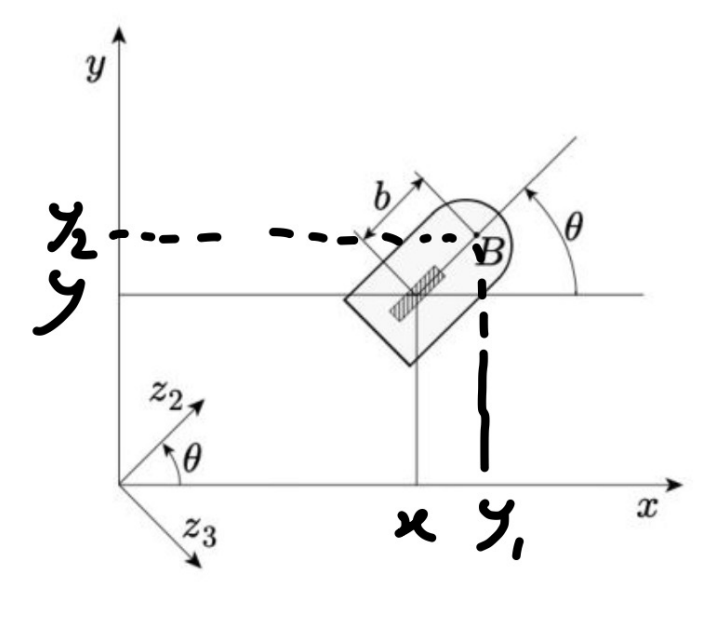
\includegraphics[width=0.6\linewidth]{Images/image25.png}
        \caption{New reference point $B$.}
        \label{fig:uni_new_ref_point}
    \end{minipage}\hfill
    \begin{minipage}{0.4\textwidth}
        Let us choose a point, $B$, located at a fixed and known distance $b$ from the center of the wheel's sagittal axis. It's coordinates with respect to an inertial reference frame are given by:
        \begin{gather*}
            y_1=x+b\cos(\theta)\\
            y_2=y+b\sin(\theta)
        \end{gather*}
    \end{minipage} 
\end{figure}
Which are chosen as outputs of the system. Then, to I/O Feedback Linearize, the outputs' derivatives are computed:
\begin{gather*}
    \begin{bmatrix}
        \dot{y}_1 \\ \dot{y}_2        
    \end{bmatrix}=
    \begin{bmatrix}
        \cos(\theta) & -b\sin(\theta) \\
        \sin(\theta) & b\cos(\theta)
    \end{bmatrix}
    \begin{bmatrix}
        v \\ \omega
    \end{bmatrix}=
    T(\theta)
    \begin{bmatrix}
        v \\ \omega
    \end{bmatrix}
\end{gather*}
Since a direct relationship between the outputs and the inputs has been obtained, the I/O Linearization transformation can be computed as:
\begin{equation*}
    \begin{bmatrix}
        v \\ \omega
    \end{bmatrix} =
    T^{-1}(\theta) 
    \begin{bmatrix}
        u_1 \\ u_2    
    \end{bmatrix}
\end{equation*}
Since $T^{-1}(\theta)$ always exists as long as $b\neq0$. The linearized system can be controlled by the simple inputs:
\begin{gather*}
    u_1 = \dot{y}_{1,d}+k_1(y_{1,d}-y_1) \\
    u_1 = \dot{y}_{2,d}+k_2(y_{2,d}-y_2) \\
\end{gather*}
With $k_1,k_2>0$, which guarantees exponential stability to the desired trajectory. However, this approach works \textit{only} for the position of the \textit{point} $B$: the orientation is uncontrolled. In fact, the closed-loop system is given as:
\begin{equation*}
    \begin{cases}
        (\dot{y}_{1,d}-\dot{y}_{1})+k_1(y_{1,d}-y_1)=0\\
        (\dot{y}_{2,d}-\dot{y}_{2})+k_2(y_{2,d}-y_2)=0\\
        \dot{\theta}= \frac{1}{b}\left\{\left[\dot{y}_{2,d}-\dot{y}_{2}\right]\cos(\theta)-\left[\dot{y}_{1,d}+k_1(y_{1,d}-y_1)\right]\sin(\theta)\right\}
    \end{cases}
\end{equation*}
\subsection{Conclusions}
In conclusion, the proposed trajectory tracking controllers have the characteristics:
\begin{itemize}
    \item Both the Linearized-based and the (Almost) nonlinear control require persistent trajectories and motion invertion is illegal.
    \item The I/O Linearization is based on a new reference point defined along the unycicle's chassis, but it is incapable of controlling the orientation of the robot.
\end{itemize}
It can also be proven that tracking the full pose of non-persistent trajectories is a \textit{structural} problem for the unicycle: due to the presence of the non-holonomic constraint, it is impossible for \textit{any} universal controller to asymptotically stabilize arbitrary full state trajectories, either persistent or not.
\subsection{Unicycle Regulation}
The \textit{regulation} problem is to get the robot from a starting configuration $q_i$ to a desired one $q_d$ without care for the trajectory in between. Again, there are different methods to achieve this.
\subsubsection{Cartesian Regulation}
Without loss of generality, assume that the desired configuration is given as $q_d=\begin{bmatrix} 0 & 0 & \theta \end{bmatrix}$. Notice that $\theta$ \textit{cannot} ben controlled, as stated in the previous sections. Define the position error:
\begin{equation*}
    e_p=
    \begin{bmatrix}
        -x & -y    
    \end{bmatrix}^{T}
\end{equation*}
Recalling the kinematic model for the unicycle eq:\ref{uni_kinematic_model}:
\begin{gather*}
    \begin{cases}
        \dot{x}_d=v_d\cos(\theta_d) \\
        \dot{y}_d=v_d\sin(\theta_d) \\
        \dot{\theta}_d=\omega_d
    \end{cases}
\end{gather*}
The following controller is designed:
\begin{gather*}
    \begin{cases}
        v=k_1(x\cos(\theta)+y\sin(\theta)) \\
        \omega=k_2(atan2(y,x)+\pi-\theta)
    \end{cases} \\
    k_1,k_2>0
\end{gather*}
Notice how:
\begin{itemize}
    \item $v$ is proportional to the projection of the error along the sagittal axis.
    \item $\omega$ is proportional to the difference between the unicycle's current orientation and the vector $e_p$ orientation. 
\end{itemize}
Stability can be proven by the Lyapunov Method and Barbalat's Lemma; consider the Lyapunov candidate function:
\begin{equation*}
    V(x)=\frac{1}{2}\left(x^2+y^2\right)
\end{equation*}
Which is positive \textit{semi}-definite, since the orientation is missing. The Lie Derivative is:
\begin{gather*}
    \dot{V}=x\dot{x}+y\dot{y}=-k_1\left[x\cos(\theta)+y\sin(\theta)\right]^{2}\leq 0
\end{gather*}
It is possible to prove that $\ddot{V}$ is bounded, so that $\dot{V}$ is uniformly continuous, then by Barbalat's Lemma $\dot{V}\rightarrow0$ for $t\rightarrow\infty$:
\begin{gather*}
    \lim_{t\rightarrow +\infty} {-k_1\left[x\cos(\theta)+y\sin(\theta)\right]^{2}}=0 \\
    x\cos(\theta)+y\sin(\theta) \rightarrow 0
\end{gather*}
So that the projection of the error $e_p$ tends to zero along the sagittal axis; however, the only point in which this can happen is the origin. In fact, any steering velocity would force the unicycle to rotate to align itself with $e_p$, which in turn would cause a change in the sagittal axis and heading velocity $v$. This is true for all initial configurations.
\subsubsection{Posture Regulation}
\begin{figure}[htbp!]
    \begin{minipage}{0.6\textwidth}
        \centering
        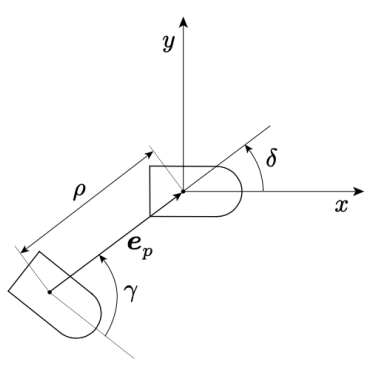
\includegraphics[width=0.5\linewidth]{Images/image26.png}
        \caption{Polar Coordinates parameterization.}
    \end{minipage}\hfill
    \begin{minipage}{0.4\textwidth}
        Without loss of generality assume that $q_d=\begin{bmatrix}0 & 0 & 0\end{bmatrix}$. Let us use the following polar coordinates parameterization:
        \begin{gather*}
            \rho=\sqrt{x^2+y^2}=|e_p| \\
            \gamma=atan(y,x)-\theta+\pi\\
            \delta=\gamma+\theta\
        \end{gather*}
    \end{minipage} 
\end{figure}
Which gives the unicycle kinematic model in polar coordinates:
\begin{equation*}
    \begin{cases}
        \dot{\rho}=-v\cos(\gamma)\\
        \dot{\gamma}=\frac{\sin(\gamma)}{\rho}v-\omega\\
        \dot{\delta}=\frac{\sin(\gamma)}{\rho}v
    \end{cases}
\end{equation*}
Notice the singularity for $\rho=0$. The following feedback controller can be designed:
\begin{gather*}
    v=k_{1}\rho\cos(\gamma)\\
    \omega=k_{2}\gamma+k_{1}\sin(\gamma)\cos(\gamma)\left[1+k_{3}\frac{\delta}{\gamma}\right] \\
    k_{1},k_{2},k_{3}>0
\end{gather*}
Giving the closed-loop system:
\begin{gather*}
    \begin{cases}
        \dot{\rho}=-k_{1}\rho\cos^{2}(\gamma)\\
        \dot{\gamma}=-k_{2}\gamma-k_{1}k_{3}\delta\cos(\gamma)\text{sinc}(\gamma)
    \end{cases}
\end{gather*}
Again, Lyapunov method and Barbalat's Lemma give the proof of stability. Let:
\begin{equation*}
    V=\frac{1}{2}\left(\rho^{2}+\gamma^{2}+k_{3}\delta^{2}\right)
\end{equation*}
Which is positive definite. The Lie Derivative is:
\begin{equation*}
    \dot{V}=-k_{1}\rho^{2}\cos^{2}(\gamma)-k_{2}\gamma^{2}\leq 0
\end{equation*}
Which is only \textit{semi}-negative definite, given the absence of $\delta$. It is possible to prove boundedness of $\ddot{V}$, so that $\dot{V}$ is uniformly continuous; by Barbalat's Lemma:
\begin{gather*}
    \lim_{t \rightarrow +\infty}{-k_{1}\rho^{2}\cos^{2}(\gamma)-k_{2}\gamma^{2}}=0 \rightarrow \\
    \rho \rightarrow0,\text{ } \gamma\rightarrow0
\end{gather*}
It is also possible to prove that $\delta \rightarrow 0$. \\
At this point, one should immediately question how come this controller is capable of regulating the unicycle's full pose, although it was said to be impossible. The catch resides in the discontinuity of this controller: indeed, it can be proven that \textit{any} feedback control law that can regulate the full pose of the unicycle must be necessarily discontinuous and/or time-varying, again due to the nonholonomic constraint. This is due to \textit{Brockett's necessary condition}:
\begin{definition}\label{Brocketts_necessary_condition}
    (\textit{Brockett's necessary condition}:) Let $x \in \mathbb{R}^{n}$, $u \in \mathbb{R}^{m}$ and $f:\mathbb{R}^{n}\times \mathbb{R}^{m}\rightarrow\mathbb{R}^{n}$ such that $f \in C^{1}$, i.e. continuously differentiable. If a continuously differentiable control law $u(x)$ such that it asymptotically stabilizes the equilibrium $x_0$ exists, then the image of the mapping $(x,u) \mapsto f(x,u)$ contains a neighborhood of $0 \in \mathbb{R}^{n}$.
\end{definition}
This definition is violated in underactuated driftless systems with linearly independent vector fields, such as the unicycle, meaning that it does not exist \textit{any continuous feedback controller} that can asymptotically stabilize an equilibrium point.
\section{Unicycle Localization}
The implementation of any feedback controller requires the availability of the robot model-configuration at each instant. However, for mobile robots in general, there is not the possibility to measure directly the position and the orientation with respect to a fixed world frame accurately enough, so that a localization procedure estimating the robot’s state must be implemented. Localization techniques can be divided into:
\begin{itemize}
    \item \textit{Active Localization}, based on the use of  Baesyan Filters (for example Kalman filters, Particle Filters) and proprioceptive and exteroceptive sensors.
    \item \textit{Passive Localization}, based on the use of only proprioceptive sensors.
\end{itemize}
It's easy to understand that active techniques lead to better results, at the cost of more computational complexity and, most importantly, more sensors needed. For active techniques look at the appendix.
\subsection{Passive Localization}
To locate the robot it is needed to reconstruct its movements in the environment. This is easily done (conceptually at least) if the inputs $v(t),\omega(t)$ are known at all times, since direct integration of these gives back the global position of the robot, assuming that the initial configuration and position is known. Notice however that these quantities are not known with absolute precision, since the actual motors used to implement the control input are most assuredly not perfect. To solve this, the actual \footnote{Notice that even if computed, these are not the \textit{true} movements that the robot has implemented, in fact the encoders are subjected to noise, so that the measurements are not perfect. Also, the ground could be slippery, so that the true movements are off by a large amount with respect to the expected ones.}input values can be computed using the proprioceptive sensors' readings. Assume that the robot is equipped with encoders at the wheels, and notice that at time $t_k$:
\begin{equation*}
    \Delta\phi_L=\omega_LT_s, \quad \Delta\phi_R=\omega_RT_s
\end{equation*}
Where $\Delta\phi_L,\Delta\phi_R$ are the left and right encoders' measurements, $T_s$ is the sampling time. Since:
\begin{equation*}
    v_k=\frac{\rho}{2}(\omega_R+\omega_L), \quad \omega_k=\frac{\rho}{d}(\omega_R-\omega_L)
\end{equation*}
It follows from the unicyle's kinematic model that:
\begin{equation*}
    v_k=\frac{\rho}{2T_s}(\Delta\phi_R+\Delta\phi_L),\quad \omega=\frac{\rho}{T_sd}(\Delta\phi_R-\Delta\phi_L)
\end{equation*}
Then, integration can be carried out either by the Euclidean approximation:
\begin{gather*}
    x_{k+1}=x_k+v_kT_s\cos\theta_k\\
    y_{k+1}=y_k+v_kT_s\sin\theta_k\\
    \theta_{k+1}=\theta_k+\omega_kT_s
\end{gather*}
Or by the more precise Runge-Kutta 2° order method:
\begin{gather*}
    x_{k+1}=x_k+v_kT_s\cos\left(\theta_k+\frac{1}{2}\omega_kT_s\right)\\
    y_{k+1}=y_k+v_kT_s\sin\left(\theta_k+\frac{1}{2}\omega_kT_s\right)\\
    \theta_{k+1}=\theta_k+\omega_kT_s
\end{gather*}
These methods give back weak results, generally speaking. They completely ignore the environment and measurement noise, which one should expect to be fundamental in the context of robot \textit{localization}. However, the enormous ease of implementation, reduced cost and less spatial requirements offered by these techniques make them valuable still, especially in those robots which either don't have the space to mount better sensors or even don't need to.  \newpage
\chapter{Aerial Robotics}
\section{Introduction}
The field of \textit{Aerial Robotics} has become a new frontier of Field Robotics; its main focus is the study of robotic systems capable of flight. It is easy to see how such systems could be of great help in many fields, going from aerial exploration of disaster zones, transportation, maintenance of infrastructure, logistics. There is a wide variety of aerial robots, classified by many metrics; for example, either by their level of autonomy:
\begin{itemize}
    \item UAV: \textit{Unmanned Aerial Vehicle}.
    \item UAS: \textit{Unmanned Aerial System}.
    \item RPV: \textit{Remotely Piloted System}.
    \item ROA: \textit{Remotely Operated Aircraft}.
    \item UVS: \textit{Unmanned Vehicle System}.
\end{itemize}
Or by the flying apparatus:
\begin{itemize}
    \item \textit{Fixed-wing}.
    \item \textit{Rotary-wing}.
    \item \textit{Tilted}, \textit{Tilting} configurations.
    \item \textit{Flapping wings}.
\end{itemize}
Aerial robots can also be distinguished by their highest reachable altitude, physical dimension, ecc. A recent development in this field has been \textit{Aerial Manipulation}: an aerial robot with a manipulator mounted on its chassis. 
\section{Dynamic Models}
\subsection{Introduction: Reference Frames}
Aerial Robots are very much different from wheeled ones; in fact, this difference also extends to the Frames of Reference used to localize the robot. 
\begin{figure}[htbp!]
    \begin{minipage}{0.4\textwidth}
        In the \textit{Earth Centered Inertial Frame} the frame's origin is Earth's center and the axes orientations are fixed, such that the $xy$-plane contains the Equator; the $z$-axis is positive in the direction of the North Pole.
    \end{minipage} \hfill
    \begin{minipage}{0.6\textwidth}
        \centering
        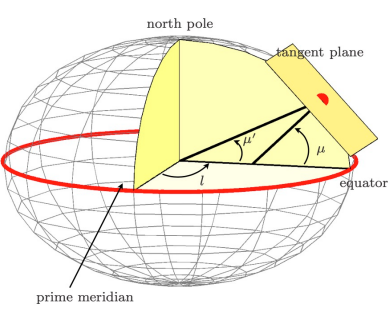
\includegraphics[width=0.6\linewidth]{Images/image27.png}
        \caption{Earth Centered Inertial FoR.}
        \label{fig:earth_centered_inertial_for}
    \end{minipage}\vfill
    \begin{minipage}{0.4\textwidth}
        The \textit{Earth Centered Earth-Fixed Frame} is mostly the same of the ECI, with the difference that the axes are moving with the Earth so that this is a non-inertial frame. GPS gives position with respect to this FoR.
    \end{minipage}\hfill
    \begin{minipage}{0.6\textwidth}
        \centering
        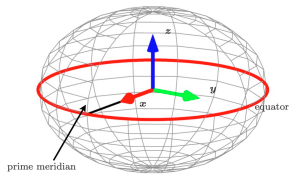
\includegraphics[width=0.6\linewidth]{Images/image28.png}
        \caption{Earth Centered Non-Inertial FoR.}
        \label{fig:earth_centered_non_inertial_for}
    \end{minipage}\vfill
    \begin{minipage}{0.4\textwidth}
        In the \textit{North-East-Down} frame the Frame of Reference is attached to a tangent plane to the Earth and is only a local description limited to the area of interest. Notice that the $z$-axis points down; the same frame of reference, but with the $z$-axis point away from the Earth's center, is called \textit{East-North-Up}.
    \end{minipage}\hfill
    \begin{minipage}{0.6\textwidth}
        \centering
        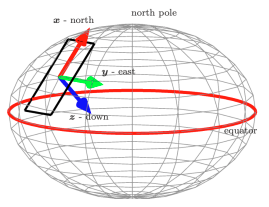
\includegraphics[width=0.6\linewidth]{Images/image29.png}
        \caption{\textit{North-East-Down} FoR.}
        \label{fig:NED_for}
    \end{minipage}
\end{figure}\\
The usual \textit{Latitude-Longitude-Altitude} or \textit{Geographic Latitude} are also used.       
\begin{figure}[htbp!]
    \begin{minipage}{0.4\textwidth}
        \centering
        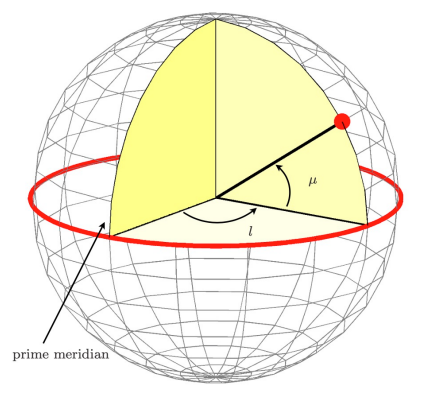
\includegraphics[width=0.4\linewidth]{Images/image30.png}
        \caption{\textit{Latitude-Longitude-Altitude} FoR.}
        \label{fig:latitude_longitude_altitude_for}
    \end{minipage} \hfill
    \begin{minipage}{0.4\textwidth}
        \centering
        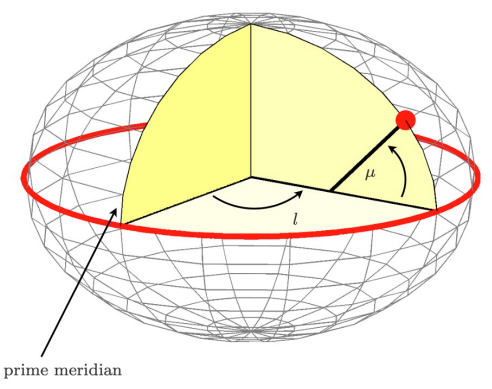
\includegraphics[width=0.4\linewidth]{Images/image31.png}
        \caption{\textit{Geographic Latitude} FoR.}
        \label{fig:geographic_latitude_for}
    \end{minipage}\vfill
\end{figure}
\subsection{Inputs}
The actuation units are mechatronic components producing thrust which typically consist of a brushless motor with a single propeller, attached to the main body either rigidly or through a mechatronic system comprising other joints and servomotors (e.g., tilted/tilting actuation units).
\begin{figure}[htbp!]
    \begin{minipage}{0.6\textwidth}
        \centering
        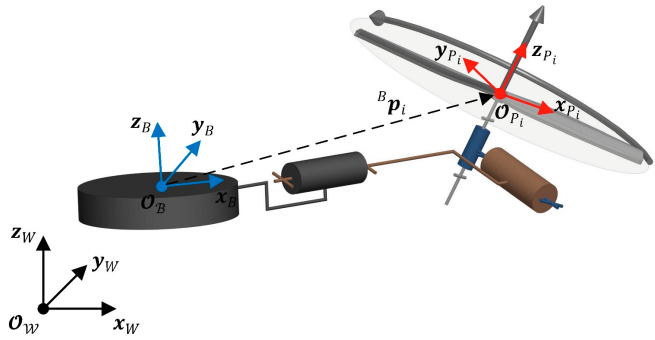
\includegraphics[width=0.6\linewidth]{Images/image33.png}
        \caption{World and Propeller Frame.}
    \end{minipage}\hfill
    \begin{minipage}{0.4\textwidth}
        For each propeller, define a frame rigidly attached to the brushless motor (not spinning with the propeller), whose position w.r.t. the body frame is given as $p_i^b$, $i\in\{1,\dots,n\}$; define the rotation axis of each motor as $z_{P_i}^{b}$. Notice that in tilting configurations (such as the one in the picture) this FoR can change its orientation, which is then given by $R_{P_i}^{b}(\alpha_i,\beta_i)\in SO(3)$, where $\alpha_i,\beta_i$ are radial and tangential rotation angles.
    \end{minipage} 
\end{figure}\\
Each propeller causes thrust and drag forces, the latter due to air resistance opposing the propeller's blades rotation. The rotation of the propeller also causes an angular momentum on the UAV's body, this is the reason why opposing propellers rotate in opposite directions: the net momentum is zero. Let us neglect:
\begin{itemize}
    \item The effects due to the propeller inertia.
    \item Flapping effects and other aerodynamic effects.
\end{itemize}
And also suppose that:
\begin{itemize}
    \item The UAV is far from obstacles. 
    \item The UAV is in a quasi-static regime (i.e. very slow).
\end{itemize}
Then, both thrust and drag can be modelled as:
\begin{equation}\label{thrust_drag_model}
    \begin{cases}
        f_{P_i}=k_{f}|\omega_i|\omega_i \\
        m_{P_i}=k_i k_{m}|\omega_i|\omega_i
    \end{cases}
\end{equation}
Where $k_{f},k_{m}>0$ are the thrust and drag factors, $k_i=1,k_i=-1$ for a descending or ascending chord, respectively. The total thrust and torque on the UAV's body is then obtained by summation:
\begin{gather*}
    f^b=\sum_{i=1}^{n}{k_{f}|\omega_i|\omega_iz_{P_i}^b}\\
    \tau^b=\sum_{i=1}^{n}{|\omega_i|\omega_i\left(-k_ik_{m}z_{P_i}^{b}+k_{f}S\left(p_{P_i}^b\right)z_{P_i}^{b}\right)}
\end{gather*}
Besides, assuming that the brushless motor are velocity controlled, it is possible to define $u_{\omega_i}=|\omega_i|\omega_i\in\mathbb{R}$ as one of the controllable inputs for the $i$-th propeller. Since it is possible to write:
\begin{equation*}
    \begin{bmatrix}
        f^b \\ \tau^b
    \end{bmatrix}=f_u(\alpha_i,\beta_i,u_{\omega_i})
\end{equation*}
The inputs are mapped from the velocity inputs $u_{\omega_i}$ by the \textit{Allocation Matrix}.
\begin{definition}\label{Allocation_Matrix}
    (\textit{Allocation Matrix}): The allocation matrix is the map $G_q:\mathbb{R}^{m_1}\rightarrow\mathbb{R}^{m_2}$, mapping the velocity inputs $u_{\omega_i}$, $i\in\{1,\dots,m_1\}$ to the vector of forces and torques $\begin{bmatrix}f^b & \tau^b\end{bmatrix}^{T}$.
\end{definition}
As an example, for a nontilting quadcopter, the allocation matrix is:
\begin{equation*}
    \begin{bmatrix}
        f_x \\ f_y \\ f_z \\ \tau_x \\ \tau_y \\ \tau_z
    \end{bmatrix}=
    \begin{bmatrix}
        0 & 0 & 0 & 0\\
        0 & 0 & 0 & 0\\
        -k_{f} & -k_{f} & -k_{f} & -k_{f}\\
        0 & -lc_f & 0 & -lc_f\\
        -k_{m} & k_{m} & -k_{m} & k_{m}
    \end{bmatrix}
    \begin{bmatrix}
        u_{\omega_1} \\ u_{\omega_2} \\ u_{\omega_3} \\ u_{\omega_4}
    \end{bmatrix}
\end{equation*}
Notice that:
\begin{itemize}
    \item Given the two null rows of the Allocation Matrix, the quadcopter is an underactuated system (the map $\dot{x}=f_u(x,u)$ is not surjective, since the nullspace of $G_q$ is not trivial).
    \item To avoid the underactuation, meaning that $G_q\in\mathbb{R}^{6\times n}$ is full column-rank, either non coplanar propellers (\textit{tilted configuration} UAVs) or motorized propellers (\textit{actively tilting configurations}) should be used.
\end{itemize}
\newpage
\subsection{Dynamic Models: non-tilting UAVs}
\begin{figure}[htbp!]
    \begin{minipage}{0.5\textwidth}
        Consider two reference frames, a \textit{Body-Fixed} frame (NED) and a \textit{World-Fixed} frame (also NED), such as in the picture. The pose of the robot can be represented by the usual position vector and rotation matrix. Assuming that the attitude has been expressed by the Euler Angles minimal representation.
    \end{minipage} \hfill
    \begin{minipage}{0.6\textwidth}
        \centering
        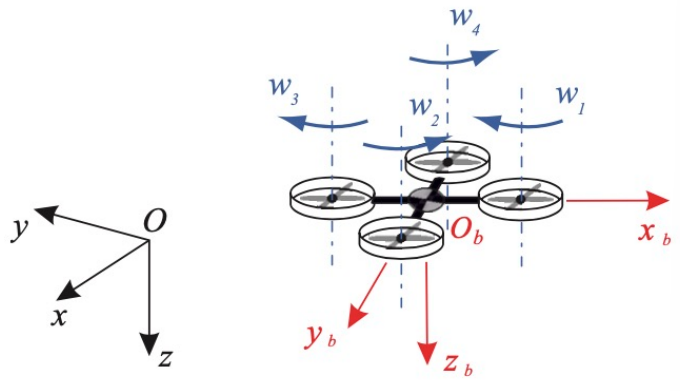
\includegraphics[width=0.6\linewidth]{Images/image32.png}
        \caption{Body and World FoR.}
    \end{minipage}
\end{figure}
\begin{gather*}
    p_b=\begin{bmatrix}
        x & y & z
    \end{bmatrix}^{T} \\
    R_b = \begin{bmatrix}
        x_b & y_b & z_b
    \end{bmatrix}\in SO(3), \\
    R_b(\eta_b)=\begin{bmatrix}
        c_{\theta}c_{\psi} & s_{\phi}s_{\theta}c_{\psi}-c_{\phi}s_{\psi} & c_{\phi}s_{\theta}c_{\psi}+s_{\phi}s_{\psi} \\
        c_{\theta}s_{\psi} & s_{\phi}s_{\theta}s_{\psi}+c_{\phi}c_{\psi} & c_{\phi}s_{\theta}s_{\psi}-s_{\phi}c_{\psi}\\
        -s_{\theta} & s_{\phi}c_{\theta} & c_{\phi}c_{\theta}
    \end{bmatrix}
\end{gather*}
Then, the dynamic model can be written with respect to the Body Frame as:
\begin{definition}\label{UAV_dyn_model_def}
    (\textit{UAV Dynamic Model}):
    \begin{equation}
        \begin{cases}\label{UAV_dyn_model}
            m\ddot{p}_{b}^{b}=-mS\left(\omega_{b}^{b}\right)\dot{p}_{b}^{b}+mgR_{b}^{T}e_{3}+f^b+f_{e}^b\\
            \dot{R}_{b}=R_{b}S\left(\omega_b^b\right)\\
            J_{b}\dot{\omega}_{b}^{b}=-S\left(\omega_b^b\right)J_{b}\omega_{b}^{b}+\tau^b+\tau_{e}^b
        \end{cases}
    \end{equation}
    Where:
    \begin{itemize}
        \item $e_3=\begin{bmatrix} 0 & 0 & 1\end{bmatrix}^{T}$\\
        \item $I_b\in\mathbb{R}^{3\times 3}$ is the diagonal inertia matrix of the body.
        \item $g$ is the constant vector of gravitational acceleration.
        \item $f_{e}^{b},\tau_{e}^{b}\in\mathbb{R}^{r}$ are external or unmodelled terms expressed in the body frame.
        \item $f_b= \begin{bmatrix}f_x & f_y & f_z \end{bmatrix}$.
        \item $\tau_b= \begin{bmatrix}\tau_x & \tau_y & \tau_z \end{bmatrix}$.
    \end{itemize}
\end{definition}
However, in terms of control systems a great simplification comes from expressing the linear motion with respect to the World Frame; by recalling that:
\begin{gather*}
    \dot{p}_b=R_b\dot{p}_{b}^{b}\rightarrow \ddot{p}_{b}=R_b\ddot{p}_{b}^{b}+R_bS\left(\omega_{b}^{b}\right)\dot{p}_{b}^{b}\
\end{gather*}
Multiplying both sides of the linear dynamics by $R_b$ and substituting:
\begin{gather*}
    mR_b\ddot{p}_b^b=-mR_bS\left(\omega_b^b\right)\dot{p}_b^b+mgR_bR_b^Te_3+R_bf^b+R_bf_e^b\rightarrow\\
    m\left(\ddot{p}_b-R_bS\left(\omega_b^b\right)\dot{p}_b^b\right)=mR_bS\left(\omega_b^b\right)\dot{p}_b^b+mgR_bR_b^Te_3+R_bf^b+R_bf_e^b
\end{gather*}
The \textit{Geometric Dynamic Model} for an UAV is obtained.
\begin{definition}\label{UAV_geomtric_dyn_model_def}
    (\textit{Geometric Dynamic Model} of an UAV):
    \begin{gather}\label{UAV_geomtric_dyn_model}
        \begin{cases}
            m\ddot{p}_b=mge_3+R_bf^b+f_e\\
            \dot{R}_b=R_bS\left(\omega_b^b\right)\\
            I_b\dot{\omega}_b^b=-S\left(\omega_b^b\right)I_b\omega_b^b+\tau^b+\tau_e^b
        \end{cases}
    \end{gather}
\end{definition}
Lastly, the model can be formulated with respect to the Euler's Angles; notice that:
\begin{equation*}
    \omega_b^b=Q(\eta_b)\dot{\eta}_b\rightarrow\ddot{\eta}_b=\dot{Q}^{-1}\omega_b^b+Q^{-1}\dot{\omega}_b^b
\end{equation*}
Provided that $\theta\neq\pm\pi/2$. The idea is to replace the coordinate-free quadrotor dynamic model to the vector $\dot{\omega}_b^b$:
\begin{gather*}
    \ddot{\eta}_b=\dot{Q}^{-1}\omega_b^b+Q^{-1}\dot{\omega}_b^b\rightarrow\\
    \ddot{\eta}_b=\dot{Q}^{-1}\omega_b^b+Q^{-1}\left[-S\left(\omega_b^b\right)I_b\omega_b^b+\tau^b+\tau_e^b\right] \rightarrow \\
    \left\{Q^{T}I_bQ\right\}\ddot{\eta}_b=\left\{Q^{T}I_bQ\right\}\dot{Q}^{-1}\omega_b^b+\left\{Q^{T}I_bQ\right\}Q^{-1}\left[-S\left(\omega_b^b\right)I_b\omega_b^b+\tau^b+\tau_e^b\right] \rightarrow \\
\end{gather*}
Since $\dot{Q}=-Q\dot{Q}^{-1}Q\rightarrow\dot{Q}^{-1}Q=-Q^{-1}\dot{Q}$ holds, it follows and defining $M\left(\eta_b\right)=\left\{Q^{T}I_bQ\right\}$:
\begin{gather*}
    M\left(\eta_b\right)\ddot{\eta}_b=Q^{T}I_b\dot{Q}\dot{\eta}_b+Q^{T}\left[-S\left(Q\dot{\eta}_b\right)I_bQ\dot{\eta}_b+\tau^b+\tau_e^b\right]
\end{gather*}
Then, the \textit{RPY dynamic model} is obtained.
\begin{definition}\label{UAV_RPY_dyn_model_def}
    (\textit{RPY dynamic model} of an UAV):
    \begin{equation}\label{UAV_RPY_dyn_model}
        \begin{cases}
            m\ddot{p}_b=mge_3+R_bf^b+f_e\\
            M(\eta_b)\ddot{\eta}_b=-C(\eta_n,\dot{\eta}_b)\dot{\eta}_b+Q^{T}(\eta_b)\tau^b+Q^{T}(\eta_b)\tau_e^b
        \end{cases}
    \end{equation}
    Where:
    \begin{itemize}
        \item $M(\eta_b)=Q^{T}(\eta_b)I_bQ(\eta_b)\in\mathbb{R}^{3\times 3}$ is symmetric and positive definite, provided that $\theta=\pm\pi/2$.
        \item $C(\eta_b,\dot{\eta}_b)=Q^{T}(\eta_b)\cdot S(Q(\eta_b)\dot{\eta}_b)\cdot I_b \cdot Q(\eta_b)+Q^{T}(\eta_b)\cdot I_b\cdot \dot{Q}(\eta_b) \in \mathbb{R}^{3\times 3}$ and $S(\cdot )\in \mathbb{R}^{3\times 3}$ is the skew-symmetric operator representing vector product.
        \item $Q(\eta_b)\in\mathbb{R}^{3\times 3}$ is the transformation matrix such that $\omega_b^b=Q(\eta_b)\dot{\eta}_b$.
    \end{itemize}
\end{definition}
The model can also be expressed in compact form:
\begin{equation}\label{UAV_RPY_compact_model}
    M_\zeta\ddot{\zeta}+C_\zeta\dot{\zeta}+g_\zeta=\Lambda u+\xi_e
\end{equation}
Where:
\begin{itemize}
    \item $M_\zeta=\begin{bmatrix}
        mI_3 &0_{3\times 3} \\ 0_{3\times 3} & M(\eta_b)
    \end{bmatrix}$
    \item $C_\zeta=\begin{bmatrix}
        0_{3\times 3} & 0_{3\times 3} \\ 0_{3\times 3} & C(\eta_b, \dot{\eta}_b)
    \end{bmatrix}$
    \item $g_\zeta=\begin{bmatrix}
        mge_3 \\0_3
    \end{bmatrix}$
    \item $\Lambda=\begin{bmatrix}
        R_b & 0_{3\times 3}\\0_{3\times 3} & Q^{T}(\eta_b)
    \end{bmatrix}\in\mathbb{R}^{6\times 4}$ and $u=\begin{bmatrix}
        \left(f^{b}\right)^{T} & \left(\tau^{b} \right)^{T}
    \end{bmatrix}$
    \item $\xi_e=\begin{bmatrix}
        f_e \\ Q^{T}(\eta_b)\tau_e^b
    \end{bmatrix} \in\mathbb{R}^{6}$
\end{itemize}
\subsection{Dynamic Models: tilting UAV}
\begin{figure}[htbp!]
    \begin{minipage}{0.7\textwidth}
        \centering
        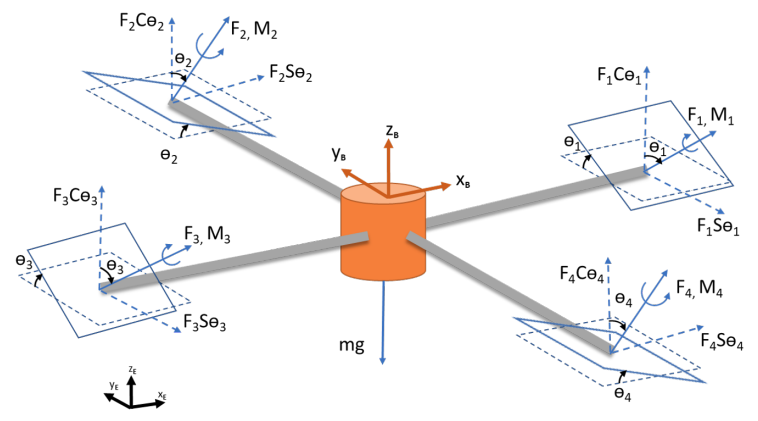
\includegraphics[width=0.7\linewidth]{Images/image34.png}
        \caption{Tilting configuration quadcopter.}
    \end{minipage}\hfill
    \begin{minipage}{0.3\textwidth}
        It is now time to introduce UAVs with tilting configurations; the Allocation matrix for a simple quadcopter with tilting configuration can be computed by drawing its free-body diagram:
    \end{minipage}
\end{figure}
\begin{definition}\label{UAV_tilting_allocation_matrix_def}
    The allocation matrix for a tilting configuration quadcopter (\textit{Holocopter method}) is:
    \begin{gather}\label{UAV_tilting_allocation_matrix_Holocopter_approach}
        G_q=
        \begin{bmatrix}
            0 & -k_{f}s_2 & 0 & k_{f}s_4\\
            k_{f}s_1 & 0 & -k_{f}s_3 & 0\\
            -k_{f}c_1 & -k_{f}c_2 & -k_{f}c_3 & -k_{f}c_4\\
            0 & -lk_{f}c_2-k_{m}s_2 & 0 &lk_{f}c_4+k_{m}s_4\\
            lk_{f}c_1+k_{m}s_1 & 0 & -lk_{f}c_3-k_{m}s_3 & 0\\
            lk_{f}c_1-c_mc_1 & -lk_{f}s_2+c_mc_2 & lk_{f}s_3-c_mc_3 & -lk_{f}s_4+c_mc_4
        \end{bmatrix}
    \end{gather}
    With the input vector defined as $u=\begin{bmatrix}
        u_{\omega_1} & u_{\omega_2} & u_{\omega_3} & u_{\omega_4}
    \end{bmatrix}$
\end{definition}
Then, the following geometric model is introduced.
\begin{definition}\label{UAV_tilting_geometric_model_def}
    (\textit{Geometric Model for a tilting quadcopter}): The \textit{Geometric Model} for a tilting configuration UAV is given by:
    \small{
    \begin{gather}\label{UAV_tilting_geometric_model}
        \begin{cases}
            \begin{bmatrix}
                mI_3 & 0 \\ 0 & I_b
            \end{bmatrix}
            \begin{bmatrix}
                \ddot{p}_b\\
                \dot{\omega}_b^b
            \end{bmatrix}=
            \begin{bmatrix}
                mge_3\\
                -S\left(\omega_b^b\right)I_b\omega_b^b
            \end{bmatrix}+
            \begin{bmatrix}
                R_b & 0 \\ 0 & I_3
            \end{bmatrix}
            \begin{bmatrix}
                G_{q,f}(\alpha) & 0\\
                G_{q,\tau}(\alpha) & 0
            \end{bmatrix}
            \begin{bmatrix}
                u_\omega\\ u_\alpha
            \end{bmatrix}\\
            \dot{R}_b=R_bS\left(\omega_b^b\right)\\ 
            \dot{\alpha}=u_\alpha
        \end{cases}
    \end{gather} }                
    Where $G_q(\alpha)=\begin{bmatrix}G_{q,f}(\alpha) \\ G_{q,\tau}(\alpha)\end{bmatrix}$ and $u_\alpha \in \mathbb{R}^4$ is the control input vector for the tilting angles.
\end{definition}
Notice that the allocation matrix in this model is \textit{not} full-rank. This is due to the tilting input $u_\alpha$ acting at a higher differential level than $u_\omega$; therefore a direct dynamics inversion at acceleration level involves only $u_\omega$, resulting in loss of controllability. This implies that, for Feedback Linearization, it is necessary to compute higher order Lie Derivatives until also $u_\alpha$ appears. If this is done, a new model is obtained:
\begin{gather*}
    \begin{cases}
        \begin{bmatrix}
            \ddot{p}_b \\ \ddot{\omega}_b^b
        \end{bmatrix}=b\left(R_b,\omega_b^b,\dot{\omega}_b^b,\alpha,u_\omega \right)+A\left(R_b,\alpha,u_\omega\right)
        \begin{bmatrix}
            u_v\\ u_\alpha
        \end{bmatrix}\\
        \dot{R}_b=R_bS\left(\omega_b^b\right)\\
        \dot{\alpha}=u_\alpha\\
        \dot{u}_\omega=u_v
    \end{cases}\\
    A=
    \begin{bmatrix}
        mI_3 & 0 \\ 0 & I_b
    \end{bmatrix}^{-1}
    \begin{bmatrix}
        R_b & 0 \\ 0 & I_3
    \end{bmatrix}
    \begin{bmatrix}
        G_q(\alpha) & \sum_{i=1}^{4}\frac{\partial g_{q,i}(\alpha)}{\partial\alpha}u_{\omega_i}
    \end{bmatrix}
\end{gather*}
Notice how $A\in\mathbb{R}^{6 \times 8}$ has full-rank as long as $u_\omega\neq0$, meaning until the propellers don't all stop. If the task is to track the desired position, velocity, and acceleration for the translational and angular part, a classic PID controller plus jerk feed-forward can be employed; since the system is redundant with respect to the given task, it is possible to employ the redundancy to optimize additional criteria (e.g., minimizing the norm of $u_\omega$ for energy consumption).\\
However, it would be easier on the life of the designer if it was possible to directly design the input forces and torques. There is a way to do this, by redefining the allocation matrix as:
\begin{definition}\label{UAV_tilting_allocation_matrix_Voliro_approach_def}
    The modified allocation matrix (\textit{Voliro approach}) for a tilting quadcopter is given by:
    \begin{gather}\label{UAV_tilting_allocation_matrix_Voliro_approach}
        G_q=
        \begin{bmatrix}
            0 & 0 & 0 & -1 & 0 & 0 & 0 &1\\
            0 & 1 & 0 & 0 & 0 & -1 & 0 & 0\\
            -1 & 0 & -1 & 0 & -1 & 0 & -1 & 0\\
            0 & 0 & -l & -k_{m}/k_{f} & 0 & 0 & l & k_{m}/k_{f} \\
            l & k_{m}/k_{f} & 0 & 0 & -l & -k_{m}/k_{f} & 0 & 0\\
            -k_{m}/k_{f} & l & k_{m}/k_{f} & -l & -k_{m}/k_{f} & l & k_{m}/k_{f} & -l
        \end{bmatrix}
    \end{gather}
    The control input to this system $u(\alpha,u_\omega)$ is defined as:
    \begin{equation*}
        u(\alpha,u_\omega)=
        \begin{bmatrix}
            u_{v,1} & u_{l,1} & u_{v,2} & u_{l,2} & u_{v,3} & u_{l,3} & u_{v,4} & u_{l,4}
        \end{bmatrix}^{T}
    \end{equation*}
    Where $u_{v,i}=k_{f} u_{\omega_i} c_{\theta_i}$, $u_{l,i}=k_{f} u_{\omega_i} s_{\theta_i}$ for $i\in\{1,\dots,4\}$.
\end{definition}
This gives the modified model:
\begin{definition}\label{UAV_tilting_model_modified_def}
    The allocation matrix defined previously results in the modified model:
    \begin{equation}\label{UAV_tilting_model_modified}
        \begin{cases}
            m\ddot{p}_b=mge_3+R_bf^b\\
            \dot{R}_b=R_bS\left(\omega_b^b\right)\\
            I_b\dot{\omega}_b^b=-S\left(\omega_b^b\right)I_b\omega_b^b+\tau^b
        \end{cases}
    \end{equation}
\end{definition}
The inputs $f^b,\tau^b$ are then obtained by pseudo-invertion of the allocation matrix:
\begin{gather*}
    \begin{cases}
        u_{\omega_i}=\frac{1}{k_{f}}\sqrt{u_{l,i}^{2}+u_{v,i}^2}\\
        \alpha_i=atan2(u_{l,i},u_{v,i})        
    \end{cases}\\
    i\in\{1,\dots,4\}
\end{gather*}
However there are two major drawbacks to this approach:
\begin{itemize}
    \item Allocating the actuator commands using the pseudoinverse may result in inadmissible rotor speeds that are higher than physically possible.
    \item This allocation does not account for the slower dynamics of the tilting angles, which leads to forces and moments being produced in directions that have not been commanded.
\end{itemize}
\subsection{Dynamic Models: Unmanned Aerial Manipulator}
An \textit{Unmanned Aerial Manipulator} is just an UAV with a manipulator mounted on it. To model its dynamics, let us define the vector of generalized joint vector:
\begin{gather*}
    \zeta=\begin{bmatrix}
        p_{b} & \eta_{b} & q_{1} & \dots & q_{n}
    \end{bmatrix}^{T}\in\mathbb{R}^{6+n}
\end{gather*}
As usual, the robot's kinematics is referred to the world frame by the homogeneous transformation matrix:
\begin{gather*}
    T_{e}=T_{b}T_{e}^{b}, \text{  }T_{e}\in SE(3)=\mathbb{R}^{3}\times SO(3)
\end{gather*}
Where $T_{b}$ is the transformation describing the robot's pose with respect to the world frame and $T_{e}^{b}$ the one describing the end-effector's pose with respect to the body frame. The kinematics is then given by differentiation:
\begin{gather*}
    \begin{bmatrix}
        \dot{p}_{b} \\ \omega_{b}^{b} \\ \dot{p}_{e}^{b} \\ \omega_{e}^{b}
    \end{bmatrix}=
    \begin{bmatrix}
        I_{3} & 0_{3} & 0\\
        0_{3} & Q(\eta_{b}) & 0\\
        0 & 0 & J(q)
    \end{bmatrix}
\end{gather*}
Define for each link a local reference frame attached to its Center of Mass, similarly as has been done previously in the context of robotic manipulators; each CoM position is then given as:
\begin{gather*}
    p_{l_{i}}=p_{b}+R_{b}p_{b_{l_{i}}}^{b}, \text{ }i=1,\dots,n
\end{gather*}
Where $p_{b_{l_{i}}}^{b}$ is the link's CoM position with respect to the body frame. Since the generalised velocities of each link can be expressed by Jacobians and the generalised joint velocities such as:
\begin{gather*}
    \dot{p}_{b_{l_{i}}}=J_{p}^{(l_{i})}\dot{q}\\
    \omega_{b_{l_{i}}}=J_{o}^{(l_{i})}\dot{q}
\end{gather*}
The link's velocities in the World Frame are:
\begin{gather*}
    \dot{p}_{b_{l_{i}}}=\dot{p}_{b}-S\left(R_{b}p_{b_{l_{i}}}\right)\omega_{b}+R_{b}J_{p}^{(l_{i})}\dot{q}\\
    \omega_{l_{i}}=\omega_{b}-R_{b}J_{o}^{(l_{i})}\dot{q}
\end{gather*}
These are used in the Lagrangian Formalism to get the model:
\begin{gather*}
    B(\zeta)\ddot{\zeta}+C(\zeta,\dot{\zeta})\dot{\zeta}+\bar{g}(\zeta)=u
\end{gather*}
With the usual meanings for the symbols. The system's input, in the cae of a flat configuration UAV and a fully-actuated manipulator, is:
\begin{gather*}
    f=
    \begin{bmatrix}
        u_{T} & \tau^{b} & \tau_{q}
    \end{bmatrix}^{T}\in\mathbb{R}^{4+n}
\end{gather*}
Where $\tau_q\in\mathbb{R}^{n}$ are the manipulator's torques. The relationship between $u$ and $f$ is not immediate, and is given by:
\begin{gather*}
    u=diag\{R_{b}e_{3},Q^{T},I_{n}\}=\Omega f\\
    \Omega\in\mathbb{R}^{(n+6)\times(n+4)}
\end{gather*}
The control of such a system will not be part of the discussion here, however there are mainly two approaches: centralized and decentralized control. The first, which is especially useful in the case of non-tilting configurations (which are underactuated), it to directly compute the input for all propellers and the manipulator, so that the UAV and manipulator dynamics are coupled; in the case of decentralized control, the two dynamics are thought of as uncoupled.
\section{Control and Flat Outputs}
\subsection{Flat Outputs}
The quadrotor is a differentially flat system, with flat outputs $(x,y,z,\psi)$; this means that the UAV trajectory can be planned as a function of the flat outputs; still, due to the UAV's underactuation (in the case of non-tilting configurations), it is impossible to controll the full pose. \\
Let us consider the RPY model eq:\ref{UAV_RPY_compact_model}, for which the state is chosen to be $x=[\zeta,\dot{\zeta}]^{T}$; then, the diffeomorphism $\sigma:\mathbb{R}^n\rightarrow\mathbb{R}^n$ linking the state to the flat outputs is given by:
\begin{equation}\label{UAV_flat_outputs}
    \sigma=
    \begin{bmatrix}
        \sigma_1 \\ \sigma_2 \\ \sigma_3 \\ \sigma_4
    \end{bmatrix}=
    \begin{bmatrix}
        x \\ y \\ z \\ \psi
    \end{bmatrix}
\end{equation}
Its inverse is given as:
\begin{equation}\label{UAV_state_from_flat_outputs}
    \begin{cases}
        x=\sigma_1\\
        y=\sigma_2\\
        z=\sigma_3\\
        \phi=\sin^{-1}\left(\frac{\ddot{\sigma}_{2}\cos(\sigma_4)-\ddot{\sigma}_{1}\sin(\sigma_4)}{\sqrt{\ddot{\sigma}_{1}^{2}+\ddot{\sigma}_{2}^{2}+\left(\ddot{\sigma}_{3}-g\right)^{2}}}\right) \\
        \theta=\tan^{-1}\left(  \frac{\ddot{\sigma}_{1}\cos(\sigma_4)+\ddot{\sigma}_{2}\sin(\sigma_4)}{\ddot{\sigma}_3-g} \right)\\
        \psi=\sigma_4
    \end{cases}
\end{equation}
The inputs to the system then should be:
\begin{gather}\label{UAV_flat_outputs_inputs}
    \begin{cases}
        u_{T}=m\sqrt{\ddot{\sigma}_{1}^{2}+\ddot{\sigma}_{2}^{2}+\left(\ddot{\sigma}_{3}-g\right)^{2}} \\
        \tau_{b}^{b}=J_{b}\left[\dot{R}_{b}^{T}+R_{b}^{T}\ddot{R}_{b}\right]^{\vee}+R_{b}^{T}\dot{R}_{b}J_{b}\left[R_{b}^{T}\dot{R}_{b}\right]^{\vee}
    \end{cases}
\end{gather}
Where $\vee$ is the \textit{Vee-operator}, i.e. the inverse of the skew-symmetric operator. Notice that the inputs include the dynamics, which means that these inputs are only allowed if feed-forward control is sufficient.
\subsection{Hierarchical Controller of a Quadcopter}
Starting from the RPY model of eq:\ref{UAV_RPY_dyn_model}, ignoring external disturbances, it is possible to design a type of \textit{Hierarchical Controller}; its main structure is:
\begin{itemize}
    \item A linear subsystem, concerning the quadcopter's linear dynamics.
    \item A linear subsystem, concerning the quadcopter's angular dynamics.
    \item A nonlinear interconnection between the subsystems.
\end{itemize}
To this end, a feedback linearization is carried out on the angular dynamics, by the input:
\begin{equation*}
    \tau^b=J_{b}Q(\eta_b)\tilde{\tau}+Q(\eta_b)^{-T}C(\eta_b,\dot{\eta}_b)\dot{\eta}_b
\end{equation*}
Notice that there is a singularity at $\theta=\pm\pi/2$, which is not a surprise since the Euler Angles are involved in this model. Define the attitude error $e_\eta$:
\begin{gather}\label{UAV_hier_attitude_error}
    e_\eta=
    \begin{bmatrix}
        e_\phi \\ e_\theta \\ e_\psi
    \end{bmatrix}=
    \eta_n-\eta_{b,d}=
    \begin{bmatrix}
        \phi \\ \theta \\ \psi
    \end{bmatrix} -
    \begin{bmatrix}
        \phi_d \\ \theta_d \\ \psi_d
    \end{bmatrix} 
\end{gather}
The quadcopter model then becomes\footnote{Notice that in the error definition it is assumed that a desired orientation is known, although it is not controllable. This would seem a contradiction, but remember that the quadcopter is a flat system: the desired attitude can be computed by the flat outputs.
\begin{gather*}
    \varphi_d=\sin^{-1}\left[\frac{m}{u_T}\left(\cos(\psi_d)-\mu_x\sin(\psi_d)\right)\right] \\
    \theta_d=\tan^{-1}\left[\frac{\mu_x\cos(\psi_d)+\mu_y\sin(\psi_d)}{\mu_z-g}\right]
\end{gather*}
Notice the singularity for $\mu_z=g$; the planner should avoid this by committing to the constraint $|\mu_z|<g$.
}:
\begin{gather*}
    \begin{cases}
        \ddot{p}_b=\left\{-\frac{1}{m}u_{T}R_b(\eta_{b,d})e_3+ge_3\right\}+\frac{1}{m}u_{T}\delta(\eta_{b,d},\eta_{n})\\
        \ddot{\eta}_b=\tilde{\tau}\\
        \delta(\eta_{b,d},e_\eta)=
        \begin{bmatrix}
            s_{\phi_d}s_{\psi_d}-s_{\phi}s_{\psi}-c_{\phi}c_{\psi}s_{\theta}+c_{\phi_d}c_{\psi_d}s_{\theta_d}\\
            c_{\psi}s_{\theta}-s_{\phi_d}c_{\psi_d}+c_{\phi_d}s_{\psi_d}s_{\theta_d}-c_{\phi}c_{\psi}s_{\theta}\\
            c_{\phi_d}c_{\theta_d}-c_{\phi}c_{\theta}
        \end{bmatrix}
    \end{cases}
\end{gather*}
Resulting in:
\begin{equation}\label{UAV_hierachical_interconnection_model}
    \begin{cases}
        \ddot{p}_b=\mu_d+\frac{1}{m}u_{T}\delta(\eta_{b,d},\eta_{n})\\
        \ddot{\eta}_b=\tilde{\tau}\\
        \delta(\eta_{b,d},e_\eta)=
        \begin{bmatrix}
            s_{\phi_d}s_{\psi_d}-s_{\phi}s_{\psi}-c_{\phi}c_{\psi}s_{\theta}+c_{\phi_d}c_{\psi_d}s_{\theta_d}\\
            c_{\psi}s_{\theta}-s_{\phi_d}c_{\psi_d}+c_{\phi_d}s_{\psi_d}s_{\theta_d}-c_{\phi}c_{\psi}s_{\theta}\\
            c_{\phi_d}c_{\theta_d}-c_{\phi}c_{\theta}
        \end{bmatrix}
    \end{cases}
\end{equation}
Where $\delta(\eta_{b,d},e_\eta)$ is the nonlinear connection between the two linear subsystems mentioned earlier. The error dynamics are easily found from the linearized system:
\begin{gather*}
    \begin{cases}
        \begin{bmatrix}
            \dot{e}_p \\ \ddot{e}_p
        \end{bmatrix}=
        \begin{bmatrix}
            0 & I \\ 0 & 0
        \end{bmatrix}
        \begin{bmatrix}
            e_p \\ \dot{e}_p
        \end{bmatrix}+
        \begin{bmatrix}
            0 \\ I
        \end{bmatrix}
        \left(\mu_d-\ddot{p}_{b,d}\right)+\frac{1}{m}u_{T}
        \begin{bmatrix}
            0 \\ \delta(\eta_{b,d},e_\eta)
        \end{bmatrix}\\
        \begin{bmatrix}
            \dot{e}_\eta \\ \ddot{e}_\eta
        \end{bmatrix}=
        \begin{bmatrix}
            0 & I \\ 0 & 0
        \end{bmatrix}
        \begin{bmatrix}
            e_\eta \\ \dot{e}_\eta
        \end{bmatrix}+
        \begin{bmatrix}
            0 \\ I
        \end{bmatrix}
        \left(\tilde{\tau}-\ddot{\eta}_{b,d}\right)
    \end{cases} \rightarrow \\
    \begin{cases}
        \begin{bmatrix}
            \dot{e}_p \\ \ddot{e}_p
        \end{bmatrix}=A
        \begin{bmatrix}
            e_p \\ \dot{e}_p
        \end{bmatrix}+B
        \left(\mu_d-\ddot{p}_{b,d}\right)+\frac{1}{m}u_{T}
        \Delta\\
        \begin{bmatrix}
            \dot{e}_\eta \\ \ddot{e}_\eta
        \end{bmatrix}=A
        \begin{bmatrix}
            e_\eta \\ \dot{e}_\eta
        \end{bmatrix}+B
        \left(\tilde{\tau}-\ddot{\eta}_{b,d}\right)
    \end{cases}
\end{gather*}
The system can be stabilized by the simple controller:
\begin{gather*}
    \begin{cases}
        \mu_d=-K_p
        \begin{bmatrix}
            e_p \\ \dot{e}_p
        \end{bmatrix} + \ddot{p}_{b,d}\\
        \tilde{\tau}=-K_{e}
        \begin{bmatrix}
            e_\eta \\ \dot{e}_\eta
        \end{bmatrix}+\ddot{\eta}_{b,d}
    \end{cases}
\end{gather*}
With $K_p,K_e\in\mathbb{R}^{3\times 6}$ are chosen such that $A_p=A-BK_p, A_e=A-BK_e$ are Hurwitz. The resulting closed-loop system is asymptotically stable, however the asymptotically stability of the interconnection requires the use of perturbation theory and will not be addressed here. 
\begin{gather*}
    \begin{cases}
        \begin{bmatrix}
            \dot{e}_p \\ \ddot{e}_p
        \end{bmatrix}=A
        \begin{bmatrix}
            e_p \\ \dot{e}_p
        \end{bmatrix}+\frac{1}{m}u_{T}\Delta\\
        \begin{bmatrix}
            \dot{e}_\eta \\ \ddot{e}_\eta
        \end{bmatrix}=A_e
        \begin{bmatrix}
            e_\eta \\ \dot{e}_\eta
        \end{bmatrix}
    \end{cases}
\end{gather*}
In conclusion, a Hierarchical Controller is composed by:
\begin{itemize}
    \item An outer loop: given the desired linear position, velocity, and acceleration from the planner, it is possible to compute:
    \begin{equation*}
        \mu_d =
        \begin{bmatrix}
            e_p \\ \dot{e}_p
        \end{bmatrix}+\ddot{p}_{b,d}
    \end{equation*}
    Then, we find the total thrust and the reference for the roll and the pitch angles.
    \item An inner loop: once having computed the desired attitude by the flat outputs, a second-order filter is used to obtain the necessary derivatives; then $\tilde{\tau},\tau$ are computed from the linearizing feedback input formula. Then, the propellers' velocities are assigned.
\end{itemize}
\subsection{\textit{Geometric Controller} of a Quadcopter}
Consider the coordinate-free geometrical model of eq:\ref{UAV_geomtric_dyn_model}. In a geometrical controller the main objective is two-fold:
\begin{itemize}
    \item Align the body $z$-axis with a desired axis.
    \item Choose the appropriate $u_T$ to follow the desired trajectory.
\end{itemize}
This is done by appropriately choosing $u_T$ and more importantly $R_{b,d}e_3$: this last choice is critical, in the sense that it could happen that the triplet $(x_{b,d},y_{b,d},z_{b,d})$ is not mutually orthogonal. To avoid this, a projection operation is executed, defining then $R_{b,d}$ as:
\begin{equation}\label{UAV_geometric_control_desired_z}
    R_{b,d}=
    \begin{bmatrix}
        S(y_{b,d}) & \frac{S(z_{b,d})x_{b,d}}{||S(z_{b,d})x_{b,d}||} & z_{b,d}
    \end{bmatrix}
\end{equation}
Also, to ensure that the planned desired linear acceleration does not exceed $g$, assume that $||-mge_3+m\ddot{p}_{b,d}||<M$, where $M>0$.
Define the errors:
\begin{gather}\label{UAV_geometric_controller_errors}
    e_p=p_b-p_{b,d}\\
    e_{R}=\frac{1}{2}\left[R_{b,d}^{T}R_{b}-R_{b}^{T}R_{b,d}\right]^{\vee}\\
    e_{\omega}=\omega_{b}^{b}-R_{b}^{T}R_{b,d}\omega_{b,d}^{b,d}
\end{gather}
Then, the control system is composed by:
\begin{itemize}
    \item An outer-loop control, defined by:
    \begin{gather}\label{UAV_geometric_controller_outer_loop_u}
        u_{T}=-\left[-K_pe_p-K_v\dot{e}_p-mge_3+m\ddot{p}_{b,d}\right]^{T}R_be_3\\
        z_{b,d}=-\frac{-K_pe_p-K_v\dot{e}_p-mge_3+m\ddot{p}_{b,d}}{||-K_pe_p-K_v\dot{e}_p-mge_3+m\ddot{p}_{b,d}||}
    \end{gather}
    \item An inner-loop control, defined by:
    \begin{gather*}
        \tau^b=-K_Re_R-K_{\omega}e_{\omega}+S\left(\omega_{b}^{b}\right)I_b\omega_{b}^{b}-I_b\left[ S\left(\omega_{b}^{b}\right)R_{b}^{T}R_{b,d}\omega_{b,d}^{b,d}-R_{b}^{T}R_{b,d}\dot{\omega}_{b,d}^{b,d} \right]
    \end{gather*}
\end{itemize}
Under this control the closed-loop dynamics becomes:
\begin{equation*}
    m\ddot{e}_p+K_v\dot{e}_p+K_pe_p=-\frac{u_T}{e_3^TR_{b,d}^TR_be_3}\left[\left(e_3^TR_{b,d}^TR_be_3\right)R_be_3-R_{b,d}e_3\right]
\end{equation*}
Notice that the RHS plays the role of the interconnection term,  as already seen in the previous section on Hierarchial Control, which becomes zero when the error orientation is null. It is possible to prove exponential stability of the origin by means of Lyapunov Theory.
\subsection{Estimar-Based Control of a quadcopter}
Once again let us consider the RPY model of eq:\ref{UAV_RPY_dyn_model}, this time without neglecting the external disturbances. Define the generalised momentum vector:
\begin{gather}\label{UAV_estimator_based_control_gen_momentum}
    q=
    \begin{bmatrix}
        mI_3 & 0_3\\ 0_3 & M(\eta_b)
    \end{bmatrix}
    \begin{bmatrix}
        \dot{p}_b\\ \dot{\eta}_b
    \end{bmatrix}\rightarrow\\
    \dot{q}=
    \begin{bmatrix}
        mge_3-u_{T}R_be_3+f_e\\
        C^{T}(\eta_b,\dot{\eta}_b)\dot{\eta}_b+Q^{T}(\eta_b)\tau^{b}+\tau_e
    \end{bmatrix}
\end{gather}
The estimator's job is to estimate the external wrench $[f_e,\tau_e]$. For simplicity, assume a linear relationship between the external wrench and its estimation in the Laplace domain:
\begin{equation*}
    \mathcal{L}
    \begin{bmatrix}
        \begin{bmatrix}
            \hat{f}_e \\ \hat{\tau}_e
        \end{bmatrix}    
    \end{bmatrix}=
    G(s)\mathcal{L}
    \begin{bmatrix}
        \begin{bmatrix}
            f_e \\ \tau_e
        \end{bmatrix}    
    \end{bmatrix}
\end{equation*}
Where $G(s)=diag(\{G_i(s)\})$, $i\in\{1,\dots,6\}$. To further simplify, let:
\begin{equation*}
    G_i(s)=\frac{k_0}{s+c_0}, i\in\{1,\dots,6\}
\end{equation*}
The choice of the gains $k_0,c_0>0$ is critical; an obvious choice is $k_0=c_0$, which doesn't give any amplification during the estimation. Assume that the estimator is turned-on before the UAV's take-off and applying the inverse Laplace transform:
\begin{gather*}
    \frac{d}{dt}
    \begin{bmatrix}
        \hat{f}_e \\ \hat{\tau}_e    
    \end{bmatrix}=k_0 
    \begin{bmatrix}
        f_e(t) \\ \tau_e(t)
    \end{bmatrix}-
    \begin{bmatrix}
        \hat{f}_e(t) \\ \hat{\tau}_e(t)
    \end{bmatrix}\rightarrow\\
    \frac{d}{dt}
    \begin{bmatrix}
        \hat{f}_e \\ \hat{\tau}_e    
    \end{bmatrix}=k_0
    \left\{
    \dot{q}-
    \begin{bmatrix}
        mge_3-u_{T}R_be_3 \\ C^{T}(\eta_b,\dot{\eta}_b)\dot{\eta}_b+Q^{T}(\eta_b)\tau^b
    \end{bmatrix}
    \right\}-
    \begin{bmatrix}
        \hat{f}_e(t) \\ \hat{\tau}_e(t)
    \end{bmatrix}\rightarrow\\
    \begin{bmatrix}
        \hat{f}_e \\ \hat{\tau}_e    
    \end{bmatrix}=k_0
    \left\{
    \dot{q}-
    \int_{0}^{t}\left\{
    \begin{bmatrix}
        mge_3-u_{T}R_be_3 \\ C^{T}(\eta_b,\dot{\eta}_b)\dot{\eta}_b+Q^{T}(\eta_b)\tau^b
    \end{bmatrix}
    -
    \begin{bmatrix}
        \hat{f}_e(t) \\ \hat{\tau}_e(t)
    \end{bmatrix}
    dt \right\}
    \right\}
\end{gather*}
Notice that to correctly estimate the external wrench it is needed to measure:
\begin{itemize}
    \item The UAV's attitude (IMU sensor).
    \item The UAV's angular velocity (IMU sensor).
    \item The UAV's linear velocity (GPS/On-board devices).
    \item The UAV's inputs (the controller gives these directly).
    \item The UAV's model's parameters.
\end{itemize}
Obviously, higher order filters can be employed; as an example, the same procedure just outlined could be replicated with a $r$-th order estimator:
\begin{equation*}
    G_i(s)=\frac{c_0}{s^r+c_{r-1}s^{r-1}+\dots+c_1s+c_0}
\end{equation*}
Building the Hurwitz Polynomial and then the filter:
\begin{gather*}
    \sum_{i=0}^{r} \prod_{j=-r}^{-(i+1)}{K_j\frac{d^i}{dt^i}
    \begin{bmatrix}
        \hat{f}_e(t) \\ \hat{\tau}_e(t)    
    \end{bmatrix}}=
    \prod_{i=1}^{r}K_i 
    \begin{bmatrix}
        f_e(t) \\ tau_e(t)
    \end{bmatrix}\\
    \gamma_1(t)=K_1\left\{q-\int_{0}^{t}\left\{
    \begin{bmatrix}
        \hat{f}_e \\ \hat{\tau}_e
    \end{bmatrix}+
    \begin{bmatrix}
        mge_3-u_{T}R_be_3\\
        C^{T}(\eta_b,\dot{\eta}_b)\dot{\eta}_b+Q^{T}(\eta_b)\tau^b
    \end{bmatrix}
    \right\}dt
    \right\}\\
    \gamma_i(t)=K_i \int_{0}^{t}\left\{
    -\begin{bmatrix}
        \hat{f}_e\\ \hat{\tau}_e
    \end{bmatrix}+\gamma_{i-1}
    \right\}dt, i=2,\dots,r\\
    \prod_{i=j+1}^{r}K_i=c_j,j=0,\dots,r-1
\end{gather*}
\subsection{Passivity-Based Controller with Compensation of external wrench}
Let us consider once again the RPY model of a quadcopter of e1:\ref{UAV_RPY_dyn_model}. In the previous sections, the use of feedback linearization and an estimator have been illustrated. However, one of the (if not "the") flaws of I/O Feedback Linearization is its reliance of a perfect model for the UAV, although it is obviously not generally the case that a perfect model is available. If I/L FL is to be avoided, an alternative is represented by \textit{Passive Control}. In this section both a Passivity-Based Controller and the Estimator discussed in the previous section will be employed.\\
Let us design an inner/outer-loop controller; for the inner-loop define:
\begin{itemize}
    \item $\dot{\eta}_b=\dot{\eta}_{b,d}-\sigma e_\eta$, where $\sigma>0$ is a coupling parameter.
    \item $\ddot{\eta}_{r}=\ddot{\eta}_{b,d}-v\dot{e}_\eta$.
    \item $e_\eta=\eta_b-\eta_{b,d}$.
    \item $\dot{e}_\eta=\dot{\eta}_b-\dot{\eta}_{b,d}$.
    \item $v_\eta=\dot{e}_\eta+\sigma e_\eta$
\end{itemize}
Then, the control input:
\begin{gather*}
    \tau^b=Q^{-T}\left[ M(\eta_{b})\ddot{\eta}_{r}+C(\eta_b.\dot{\eta}_b)\dot{\eta}_r-\hat{\tau}_e-D_0v_\eta-K_0e_\eta \right]\\
    D_0,K_0\in\mathbb{R}^{3 \times 3}: D_0>0,K_0>0
\end{gather*}
Which will regulate the quadcopter's angular dynamics. For the outer-loop, define the errors:
\begin{itemize}
    \item $e_p=p_b-p_{b,d}$.
    \item $\dot{e}_p=\dot{p}_b-\dot{p}_{b,d}$.
    \item $\ddot{e}_p=\ddot{p}_b-\ddot{p}_{b,d}$.
    \item $\mu_d=(1/m)\left[ge_3+\hat{f}_e-u_{T}R_b(\eta_{b,d})e_3\right]$.
    \item $\tilde{f}=f_e-\hat{f}_e$, the linear estimation error.
\end{itemize}
Then, by substitution of $\eta_b=e_\eta+\eta_{b,d}$ the linear dynamics becomes:
\begin{equation*}
    \ddot{p}_b=\mu_d+\frac{1}{m}\left[\delta\cdot u_{T}+\tilde{f}\right]
\end{equation*}
Where $\delta$ is the interconnection term that was described in equations eq:\ref{UAV_hierachical_interconnection_model}; also, as in the Hierachical Control method, neglecting for a moment the underactuation of the quadcopter (remembering that the desired attitude can be however computed), define:
\begin{equation*}
    \mu_d=-K_d\dot{e}_p-K_pe_p+\ddot{p}_{b,d}
\end{equation*}
The closed-loop dynamics becomes:
\begin{gather}\label{UAV_passivity_control_closed_loop}
    m\ddot{e}_p+K_d\dot{e}_p+K_pe_p=u_{T}\delta+\tilde{f}\\
    M\dot{v}_\eta+\left(C+D_0\right)v_\eta+K_0e_\eta=\tilde{\tau}
\end{gather}
Both closed-loop equations can be seen as mass-damping-spring systems with programmable stiffness, partially-programmable damping and given mass and inertia; also, notice that:
\begin{itemize}
    \item $K_p,K_d$ have physical meanings, which is always of help for the designer.
    \item The linear part is slower than the angular one, meaning that the closed-loop linear dynamics is defined and the estimator's bandwidth can be exactly tuned to be faster that it.
    \item The coupling factor $\sigma$ should be properly tuned since it affects the tracking results dramatically; in fact, for small values of $\sigma$ the robot could start to vibrate. A common choice is $K_0=\sigma D_0$ (which is equivalent to writing a quadratic optimization problem).
\end{itemize}
Then, the total thrust can be computed from the desired acceleration vector as usual:
\begin{gather*}
    \bar{\mu}=\begin{bmatrix}
        \bar{\mu}_{x} & \bar{\mu}_{y} & \bar{\mu}_{z}
    \end{bmatrix}=
    \mu_{d}-\frac{1}{m}\hat{f}_{e}\\
    u_{T}=m\sqrt{\bar{\mu}^{2}_{x}+\bar{\mu}^{2}_{y}+\left(\bar{\mu}_{z}-g\right)^{2}}\\
    \varphi_{d}=\sin^{-1}\left(\frac{m}{u_{T}}\left[\bar{\mu}_{y}\cos(\psi_{d})-\bar{\mu}_{x}\sin(\psi_{d})\right]\right)\\
    \theta_{d}=\tan^{-1}\left(\frac{\bar{\mu}_{x}\cos(\psi_{d})+\bar{\mu}_{y}\sin(\psi_{d})}{\bar{\mu}_{z}-g}\right)
\end{gather*}
Granted that $\bar{\mu}=\mu_{d}-\frac{1}{m}\hat{f}_{e}=ge_{3}$ should be avoided. The proposed controller can be employed without the estimator of external forces following the same passages for the linear part as for the hierarchical controller.
\section{Disturbance effects}
UAVs (or UAMs) are often employed also in closed environments or have near ground tasks to complete. However, in these situation some disturbance effects arise, due to the environment constricting the propeller's air flows. In this section, some of these effects will be investigated.
\subsection{Ground Effect}
The \textit{Ground Effect} is a disturbance which arises when the UAV is flying close to the ground. The most employed theoretical result for the description of the ground effect is based on the so-called \textit{Potential Aerodynamic Assumption}, which states that the fluid is:
\begin{itemize}
    \item Inviscid.
    \item Incompressible.
    \item Irrotational.
    \item Steady.
\end{itemize}
If these assumptions are satisfied, the \textit{Method of Images}\footnote{The Method of Images is often used also in Electrostatics to compute the polarization of an infinite conducting plane due to the presence of a point-charge placed above it.} can be employed. This method consists in placing a virtual rotor on the opposite side of the ground, which is seen as a barrier, at the same distance from it as the true propeller. 
\begin{figure}[htbp!]
    \centering
    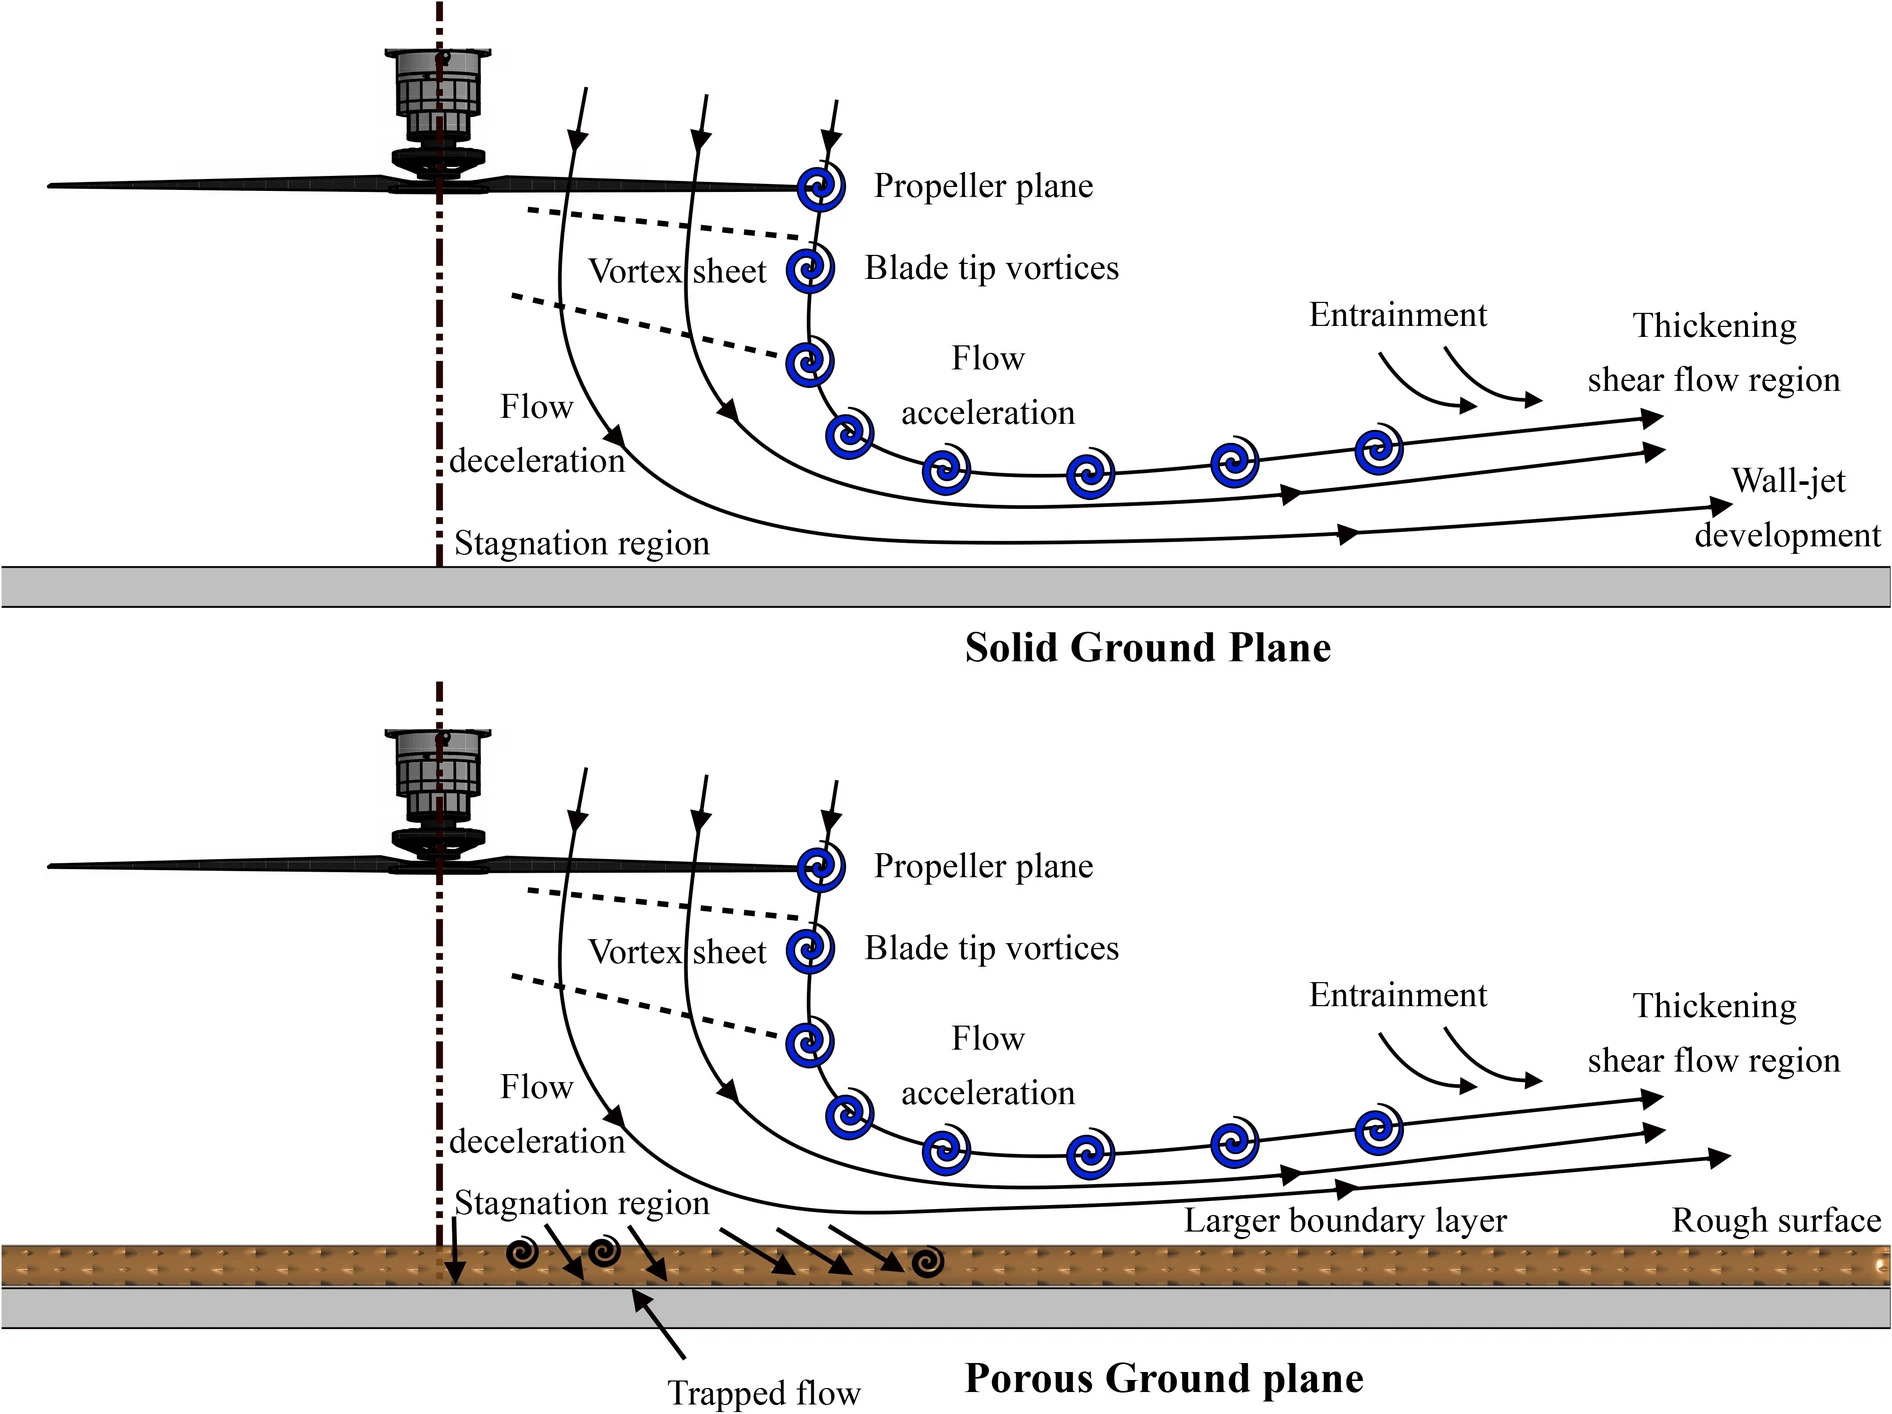
\includegraphics[width=0.6\linewidth]{Images/image35.png}
    \caption{Ground Effect for a single propeller.}
    \label{fig:groud_effect}
\end{figure}\\
Let $v_{IGE},T_{IGE}$ be the induced rotor's velocity and thrust due to the ground effect, respectively. Let $v_{OGE},T_{OGE}$ be the induced rotor's velocity and thrust without ground effect. Then, assuming power conservation between these two situations:
\begin{gather*}
    \frac{T_{IGE}}{T_{OGE}}=\frac{1}{1-\left(\frac{\rho}{4z}\right)^{2}}
\end{gather*}
Where $\rho$ and $z$ are the propeller's radius and height from the ground.
Notice that if $z/\rho=2$ then the formula gives a ratio of $1.016$, meaning that the ground effect for a single propeller is negligible if the propeller is at least two times $\rho$ above ground. The result can be specialized to the case of a quadrotor by simply considering the contributions of each propeller and conservation of power; then:
\begin{gather*}
    \frac{u_{T,IGE}}{u_{T,OGE}}=\frac{1}{1-\left(\frac{\rho}{4z}\right)^{2}-\frac{z\rho^{2}}{\sqrt{\left(d^{2}+4z^{2}\right)^{3}}}-\frac{z\rho^{2}}{2\sqrt{2\left(2d^{2}+4z^{2}\right)^{3}}}}
\end{gather*}
Ground effect causes a net torque around the UAV. This destabilizes the UAV, which tilts and reinforces the Ground effect; this can lead to instability. This is even more annoying in the case of UAMs, which would then rotate away from the object that they are trying to grasp.
\begin{figure}[htbp!]
    \begin{minipage}{0.5\textwidth}
        \centering
        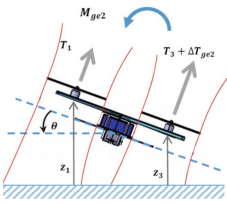
\includegraphics[width=0.6\linewidth]{Images/image36.png}
        \caption{UAV subjected to \\ Ground Effect.}
    \end{minipage}\hfill
    \begin{minipage}{0.5\textwidth}
        \centering
        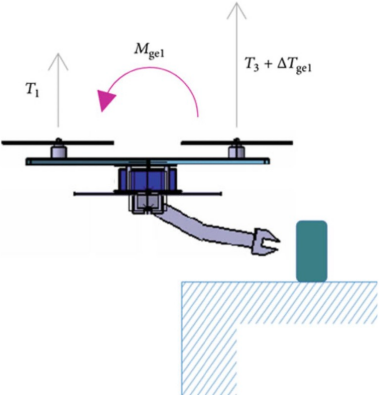
\includegraphics[width=0.5\linewidth]{Images/image37.png}
        \caption{UAM subjected to \\ Ground Effect.}
    \end{minipage} 
\end{figure}
\subsection{Ceiling Effect}
Similar to the Ground Effect, there is also a \textit{Ceiling Effect} which arises when a UAV (or UAM) fly just below a barrier. In the single rotor case, it happens that the thrust increases significantly closes to the ceiling, pushing the rotor even closer to it: this is easily understood by noticing that if the propeller pushes air against the barrier, then a low pressure volume is created above the UAV, which in turn makes the propellers blades spin faster (less air to move out of the way of each blade) increasing its thrust and creating a vacuum (this is called \textit{Vacuum Effect}). Again, this can be mathematically described as:
\begin{gather*}
    \frac{T_{ICE}}{T_{OCE}}=\frac{1}{1-\frac{1}{k_{1}}\left(\frac{\rho}{z+k_{2}}\right)^{2}}
\end{gather*}
Where $T_{ICE},T_{OCE}$ are the thrust with and without Ceiling Effect, respectively; $k_{1}, k_{2}$ are parameters to be tuned. Notice that this effect can be rendered useful by designing the propeller's velocity to make use of the increased thrust, so that a less energy costly and longer flight can be achieved.
\subsection{Wall, Pipe Effects and Flapping Dynamics}
At last, similar to Ground and Ceiling effect, there also exist the so-called \textit{Wall} and \textit{Pipe} effects, whose names are self-explanatory.\\
Much more interesting is the effect of \textit{Flapping Dynamics}, which is an undesirable effect linked to the propeller's blades high rotational velocities. 
\begin{figure}[htbp!]
    \begin{minipage}{0.5\textwidth}
        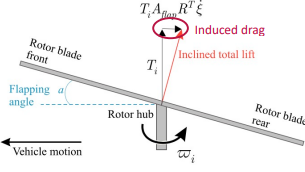
\includegraphics[width=0.75\linewidth]{Images/image38.png}
        \caption{Enter Caption}
    \end{minipage}\hfill
    \begin{minipage}{0.5\textwidth}
        The blades' flapping can be linked to their (however small) elasticity. This flapping causes a different drag force than expected, often neglected since its dissipative nature often actually helps in keeping the UAV stable. However, since each propeller is subjected to these forces, there could be a net torque on the UAV's body, especially during forward motion.
    \end{minipage} 
\end{figure}
Specifically, the advancing rotor blade has a higher velocity then the rear one and it will generate e lift force; in turn, this creates a bigger induced drag than the rear blade resulting in a net force that is opposite to the current forward motion. \newpage
\chapter{Underwater Robotics}
\section{Introduction}
Although robots can roam around the ground or even fly, most of the Earth's surface is covered in water. This immediately highlights the need for robots to become capable of handling such environments; this is the objetive of \textit{underwater robotics}. Similarly as in the case of aerial robotis, underwater robots can be classified as:
\begin{itemize}
    \item \textit{Remotely Operated Vehicles}, which are connected by a tether to an operator or surface ship.
    \item \textit{Autonomous Underwater Vehicles}.
    \item \textit{Unmanned Underwater Vehicles}.
    \item \textit{Underwater Vehicle-Manipulator Systems}.
\end{itemize}
In general, design of underwater robots is more difficult than ground or aerial ones:
\begin{itemize}
    \item GPS doesn't work underwater. \textit{Sonars} are employed.
    \item There is no single proprioceptive sensor for localization.
    \item Visibility is often scarse.
    \item Sonars are noisy sensors.
    \item The allocation matrix is very difficult to obtain, due to the highly nonlinear relationship between force/moment acting along the body and the control inputs.
\end{itemize}
\section{Dynamic Model}
The dynamic model is fairly similar to the one of an UAV, although the gravity term is missing and requires special care. 
\begin{figure}[htbp!]
    \begin{minipage}{0.6\textwidth}
        \centering
        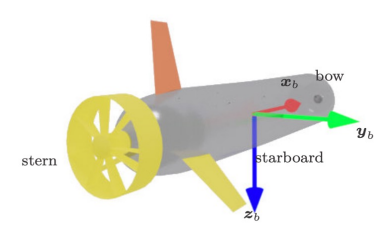
\includegraphics[width=1\linewidth]{Images/body_underwater.png}
        \caption{Underwater robot's\\ body frame.}    
    \end{minipage}
    \hfill               
    \begin{minipage}{0.4\textwidth}
        Another difference stands in the name of the angles used to represent angular motion; in underwater robotics, Roll-Pitch-Yaw angles are substituted by \textit{Surge-Sway-Heave} angles.
        \begin{itemize}
            \item \textit{Surge} along the $x$-axis.
            \item \textit{Sway} along the $y$-axis.
            \item \textit{Heave} along the $z$-axis.
        \end{itemize}
    \end{minipage}
\end{figure}
The dynamics model is then given.
\begin{definition}
    \textit{Underwater Robot's Dynamic Model}:
    \begin{gather}\label{underwater_robot_dyn_mod}
        \begin{bmatrix}
            mI_{3} & 0_3 \\
            0_3 & J_{b}
        \end{bmatrix}
        \begin{bmatrix}
            \ddot{p}_{b}^{b}\\
            \dot{\omega}_{b}^{b}
        \end{bmatrix}+
        \begin{bmatrix}
            mS(\omega_{b}^{b}) & 0\\
            0 & S(\omega_{b}^{b})J_b
        \end{bmatrix}=
        \begin{bmatrix}
            f^b \\ \tau^b
        \end{bmatrix}\\
        \dot{R}_b=R_bS(\omega_b^b)
    \end{gather}
\end{definition}
\subsection{Working in water: currents, buoyancy and added inertia}
Underwater robots have another difficulty to overcome: to achieve their movement, they also have to push the water in front of them. This implies:
\begin{itemize}
    \item An added inertia has to be considered, since the water applies reaction forces on the robot's body. This is the \textit{Added Mass Contribution}, which is a function of the body's geometry. This also implies that its associated mass matrix is not necessarily positive-definite or symmetric. 
    \item The presence of fluid causes drag and lift on the body. These effect are often lumped into a constant damping term.
\end{itemize}
Other significant contributions to the robot's dynamics are given by the presence of wind and currents. In particular, currents, $v_c$, can be assumed as irrotational and constant, then added to the model before computing the Coriolis, centripetal and damping terms:
\begin{gather*}
    v_r=\begin{bmatrix}
        \dot{p}_b^b\\ \omega_b^b
    \end{bmatrix}-R_b^Tv_c
\end{gather*}
Finally, the robot's buoyancy has to be taken into account. Notice that this is a \textit{hydrostatic} effect, meaning that it does not depend on the robot's speed. Define $b=\rho\Delta\|g\|$ to be the buoyancy force exerted on the body, which is submerged in a liquid of density $\rho$ for a certain amount $\Delta$ of its own volume. Then, the resulting wrench acting on the body expressed in the world-frame is:
\begin{gather*}
    g_{rb}^b=-
    \begin{bmatrix}
        f_g^b+f_b^b\\
        S(r_c^b)f_g^b+S(r_b^b)f_b^b
    \end{bmatrix}
\end{gather*}
Which is taken into account in the following UUV model:
\begin{definition}
    \textit{UUV Dynamic Model with buoyancy and current contribution in World-Frame:}
    \begin{gather}
        M_v
        \begin{bmatrix}
            \ddot{p}_b^b\\ \dot{\omega}_b^b
        \end{bmatrix}+(C_v+D_{RB})
        \begin{bmatrix}
            \dot{p}_b^b\\ \omega_b^b
        \end{bmatrix}+g_{rb}^b=\tau_v-\tau_{v,c}\\
        M_v=M_v^T,\quad D_{RB}>0,\quad C_v=-C_v^T
    \end{gather}
    Where $\tau_v$ is often taken to be:
    \begin{equation}
        \tau_v=B_vu_v
    \end{equation}
    Where $B_v$ is the \textit{Thrusters Control Matrix}.
\end{definition}
The model can be written with respect to the body-frame by finding a set of parameters $\theta_v$ for which it is linear. In that case, a regressor matrix can be found such that:
\begin{equation*}
    \phi_v\theta_v=\tau_v
\end{equation*}
It is useful to separate the \textit{persistent dynamics}, the one which affects the robot even when it is still, from the general dynamics; this results in the following model.
\begin{definition}
    \textit{UUV Dynamic Model with buoyancy and current contribution in Body-Frame:}
    \begin{gather}
        M_v
        \begin{bmatrix}
            \ddot{p}_b^b\\ \dot{\omega}_b^b
        \end{bmatrix}+(C_v+D_{RB})
        \begin{bmatrix}
            \dot{p}_b^b\\ \omega_b^b
        \end{bmatrix}+g_{rb}^b+
        \phi_{v,p}\theta_{v,p}\\
        \phi_{v,p}\theta_{v,p}=\phi_{v,r}\theta_{v,r}+\phi_{v,c}\theta_{v,c}
    \end{gather}
    Where $\phi_{v,r}$ is the regressor of the \textit{restoring} forces (buoyancy and gravity), $\phi_{v,c}\theta_{v,c}$ is the one referred to currents. If the currents are considered as constant and expressed in the world-frame, then:
    \begin{gather*}
        \phi_{v,p}=\begin{bmatrix}
            R_b^Te_3 & 0_3 & R_b^T & 0_3 \\
            0_3^T & S(R_b^Te_3) & 0_3 & R_b^T
        \end{bmatrix}
    \end{gather*}
    Otherwise:
    \begin{gather*}
        \phi_{v,p}=\begin{bmatrix}
            R_b^Te_3 & 0_3 & I_3 & 0_3 \\
            0_3^T & S(R_b^Te_3) & 0_3 & I_3
        \end{bmatrix}
    \end{gather*}
\end{definition}
Restoring forces pose a challenge both in terms of modeling and control, especially for large UUVs. In particular, restoring forces are well expressed in the body-frame, meanwhile currents are better expressed in the world-frame, this adds a layer of complexity to the modeling. Adaptive Controllers are best suited for underwater applications. \newpage
\chapter{Legged Robotics}
\subsection{Introduction}
Most of surface lands are inaccessible to wheeled robots, leading to the necessity of alternative motion systems. One of these are the so-called \textit{legged} robots, whose structure often imitates animals and/or insects. 
\subsection{Taxonomy}
There are a great many types of legged robots, classified by:
\begin{itemize}
    \item Stability of gait:
    \begin{itemize}
        \item \textit{Statically stable gait}(fig: \ref{fig:statically_stable_robot}): the robot control its locomotion such that the vertical projection of the center of gravity is always contained within the support polygon. Generally speaking, these robots are slow.
        \item \textit{Dinamically stable gait}(fig: \ref{fig:dinamically_stable_robot}): the robot is not statically balanced during the locomotion, the support polygon has degenerated to a point or a line.
    \end{itemize}
    \begin{figure}[htbp!]
        \begin{minipage}{0.5\textwidth}
            \centering
            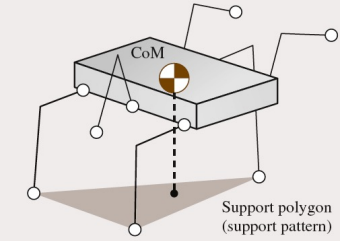
\includegraphics[width=0.5\linewidth]{Images/statically_stable_robot.png}
            \caption{Support Poligon for\\ statically stable robot.} 
            \label{fig:statically_stable_robot}
        \end{minipage}\hfill 
        \begin{minipage}{0.5\textwidth}
            \centering
            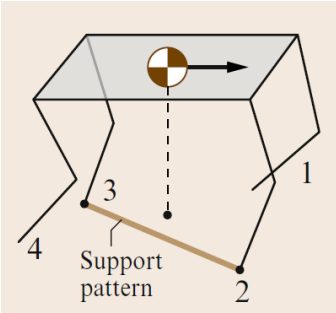
\includegraphics[width=0.5\linewidth]{Images/dinamic_stable_gait.png}
            \caption{Support Poligon for\\ dinamically stable robot.}
            \label{fig:dinamically_stable_robot}
        \end{minipage}
    \end{figure}
    \item Number of legs: monopod, bipod, etc.
    \item Type of leg articulation:
    \begin{figure}[htbp!]
        \begin{minipage}{0.7\textwidth}
            Mainly composed by a rotating and a linear actuator. It's the simplest structure possible, which however leads to low adaptability to uneven terrains.
        \end{minipage}\hfill 
        \begin{minipage}{0.3\textwidth}
            \centering
            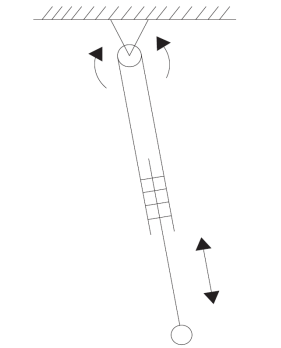
\includegraphics[width=0.5\linewidth]{Images/prismatic_leg.png}
            \caption{Prismatic Leg.}
            \label{fig:prismatic_leg}
        \end{minipage}\vfill 
        \begin{minipage}{0.4\textwidth}
            \centering
            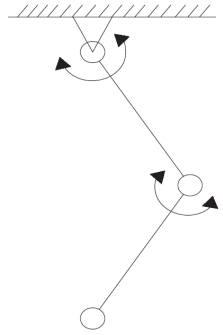
\includegraphics[width=0.4\linewidth]{Images/articulated_leg.png}
            \caption{\\Articulated Leg.}
            \label{fig:articulated_leg}
        \end{minipage}\hfill
        \begin{minipage}{0.6\textwidth}
            Compared with prismatic legs, the articulated leg uses a rotating joint instead of a linear prismatic joint to achieve leg length control. It is usually used in robot with four and more legs, with the addition of a perpendicular joint that enables the lateral motion.
        \end{minipage}\vfill 
        \begin{minipage}{0.7\textwidth}
            The extension of the articulated legs with at least one more rotating joint. Usually used in biped robots, with the addition of other joints along the different axes that are useful to improve the stability.
        \end{minipage}\hfill
        \begin{minipage}{0.3\textwidth}
            \centering
            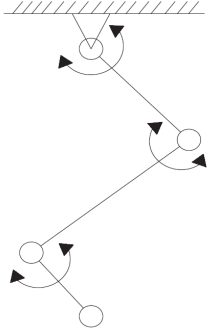
\includegraphics[width=0.5\linewidth]{Images/redundant_articulated_leg.png}
            \caption{\\Redundant\\ Articulated Leg.}
            \label{fig:redundant_articulated_leg}
        \end{minipage}
    \end{figure}
\end{itemize}

For the specific instance of quadruped robots, there is also another distinction based on the structure of the leg kinematic chain.
\begin{itemize}
    \item Forward elbow, backward knee: the optimal configuration, giving better locomotion stability and little impact force between foot and ground.
    \item Forward knee, backward elbow.
    \item Knees.
    \item Elbows.
\end{itemize}
Control also represents a challenge, since there is a need to maximize torque, bandwidth, and power meanwhile minimizing friction, inertia, and mass loss. New actuators designs are also needed to reduce the effects of the high mechanical impedance resulting from the impact with the ground, such as \textit{Series Elastic Actuators} or \textit{Proprioceptive Actuators}. Finally, navigation causes the need of a large amount of onboard sensors, many of which highly complex and costly (such as LIDARs).
\subsection{Dynamic Model}
A legged robot's configuration is fully described by the coordinates of its \textit{floating base} (the body) and the configurations of its legs.
\begin{figure}[htbp!]
    \begin{minipage}{0.5\textwidth}
        \centering
        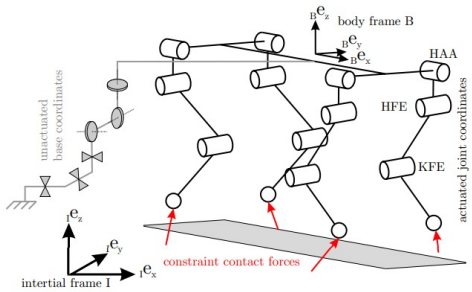
\includegraphics[width=1\linewidth]{Images/floating_base_scheme.png}
        \caption{Legged robot structure.}
        \label{fig:floating_base_scheme}
    \end{minipage}\hfill
    \begin{minipage}{0.5\textwidth}
        The former is accomplished by defining the vectors of  $p_b\in\mathbb{R}^3,R_b\in SO(3)$ describing position and orientation of the body frame with respect to the world frame, as usual; the latter, is obtained by defining the generalized coordinate vector $q=[q_b^T, q_j^T]^T\in\mathbb{R}^{n_b+n_j}$, of which the dimension is dependent on the choice of rotation parameterization.
    \end{minipage} 
\end{figure}\\
Usually, if a minimal representation is used, $q_b=[p_b^T,\eta_b^T]^T\in\mathbb{R}^6$, where $\eta_b$ are the Euler angles. Once a description of the structure is obtained, it is now possible to describe the robot's motion. A distinction between \textit{stance feet}, the ones touching the ground, and \textit{swing feet}, the ones who don't, is needed; then, the contacts are modeled as kinematic constraints imposed on the stance feet.
\begin{figure}[htbp!]
    \begin{minipage}{0.5\textwidth}
        \centering
        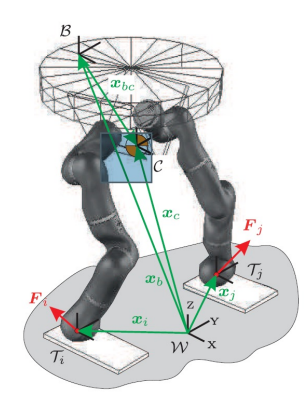
\includegraphics[width=0.75\linewidth]{Images/stance feet.png}
        \caption{Stance feet.}
        \label{fig:stance_feet}
    \end{minipage}\hfill
    \begin{minipage}{0.5\textwidth}
        \begin{definition}
            (\textit{Contact point constraint}): During robot's operation, for the $i$-th stance foot, it must hold the following \textit{non-slipping constraint}:
            \begin{gather}
                p_i=const,\quad
                \dot{p}_i=0_3,\quad
                \ddot{p}_i=0_3
            \end{gather}
            Which can be expressed a \textit{contact Jacobian} mapping the robot's generalized velocity vector into the stance feet generalized velocity vector:
            \begin{equation}\label{contact_jacobian}
                J_{T_i}=
                \begin{bmatrix}
                    \begin{bmatrix}
                        I_3 & S(p_{bi}) \\
                        0_{3\times 3} & I_{3}
                    \end{bmatrix} & J_i       
                \end{bmatrix}\in\mathbb{R}^{6\times(n_b+n_j)}
            \end{equation}
            Where $p_{bi}=p_b-p_i,J_i=\partial(r_i-q_b)/\partial q_j\in\mathbb{R}^{6\times n_j}$ and $r_i$ is the vector of the $i$-th stance foot's pose.
        \end{definition}
    \end{minipage} 
\end{figure}\\
In the particular case of a quadruped robot, the pose of the foot coincides with its position, so that the contact Jacobian becomes:
\begin{gather}\label{point_contact_Jacobian_for_quadruped_robot}
    J_{T_i}=
    \begin{bmatrix}
        I_3 & S(p_{bi}) & J_{p,i}
    \end{bmatrix}\in\mathbb{R}^{3\times (n_b+n_j)}
\end{gather}
Where $J_{p,i}$ is composed of only the first three rows of $J_i$. For an $n_{st}$ stance feet robot, the contact Jacobians are stacked into a single Jacobian:
\begin{gather}\label{total_contact_jacobian}
    J_{st}=
    \begin{bmatrix}
        J_{st,b} & J_{st,i}
    \end{bmatrix}\in\mathbb{R}^{3n_{st}\times (n_b+n_j)}
\end{gather}
Obviously, the contact points cause \textit{Ground Reaction Forces}, which push against the robot legs. It is only because of these forces that a legged robot is able to move. In turn, GRFs cause friction (which is helpful in avoiding slipping) and this has to be taken into account in the model. The most basic friction model is the \textit{Coulomb Friction Model}, which states that.
\begin{definition}
    \textit{(Coulomb Friction Model)}: Define $f_x,f_y,f_z$ as the projections of the GRFs on the axes associated to the single point contact $C_i$. Then, the friction caused by the GRFs is given as:
    \begin{equation}\label{Coulomb_Friction_Model}
        \sqrt{f_x^2+f_y^2}=\mu f_z
    \end{equation}
    Where $\mu$ is the friction coefficient.
\end{definition}
Notice that the model is, geometrically speaking, a cone (from which the alternative name \textit{friction cone model}) and is nonlinear. In order to ease the real-time computation, a linear approximation is implemented by inscribing or circumscribing a pyramid shape against the cone. In particular, the stricter version (inscribing) is used and is defined as the model:
\begin{definition}
    \textit{(Inscribed Pyramidal Friction Model):}
    \begin{gather}\label{inscribed_pyramid_friction}
        |f_x|\leq \frac{\sqrt{2}}{2}\mu f_z\\
        |f_y|\leq \frac{\sqrt{2}}{2}\mu f_z
    \end{gather}
\end{definition}
\begin{figure}[h!]
    \centering
    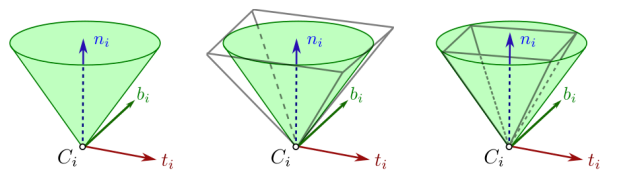
\includegraphics[width=0.75\linewidth]{Images/pyramid_friction_model.png}
    \caption{Pyramid Friction Model scheme.}
\end{figure}
Finally, the dynamic of a floating base robot can be written.
\begin{definition}
    \textit{Floating Base Robot Dynamics}:
    \begin{equation}\label{legged_robot_dynamic_model}
        M(q)\dot{v}+Cv+g=S^{T}\tau+J_{st}^{T}f_{gr}+J^{T}f_{ext}
    \end{equation}
    Where:
    \begin{itemize}
        \item $M(q)\in\mathbb{R}^{(n_b+n_j)\times(n_b+n_j)}$ is the inertia matrix.
        \item $C\in\mathbb{R}^{(n_b+n_j)\times(n_b+n_j)}$ is the Coriolis term.
        \item $g\in\mathbb{R}^{n_b+n_j}$ is the gravitational term.
        \item $S=[O_{n_j\times6},I_{n_j}]$ is the \textit{torque distribution matrix} selecting the actuated joints.
        \item $f_{gr}\in\mathbb{R}^{3n_{st}}$ is the vector of ground reaction forces (GRFs).
        \item $\tau\in\mathbb{R}^{n_j}$ is the vector of joint actuation forces.
        \item $J$ is the staked matrix of the feet Jacobians.
        \item $f_{ext}$ is the vector containing the net forces at the legs' tips accounting for unmodelled dynamics and disturbances.
    \end{itemize}
\end{definition}
\subsection{Constrained Consistent Dynamics}
A legged robot can be controlled by an inverse dynamics approach; however, the dynamic model in eq:\ref{legged_robot_dynamic_model} is not sufficient, since it does not take into account the contact constraints. A \textit{constrained consistent dynamic} model can be obtained starting from the formulation of an appropriate projection operator $N_c$, such that it takes directly into account the contact constraints. 
\begin{definition}
    \textit{(Constrained Consistent Dynamics model):} Define the model:
    \begin{equation}\label{constrained_consistent_dynamic_model}
        N_c\left(M\dot{v}+Cv+g-J^{T}f_{ext}\right)=N_cS^{T}\tau
    \end{equation}
    Where the projection operator $N_c$ is defined as:
    \begin{equation}\label{legged_robotics_dynamically_consistent_projection_operator}
        N_c=I_{n_{st}}-\left[M^{-1}J_{st}^{T}\left(J_{st}M^{-1}J_{st}^{T}\right)\right]=I_{n_{st}}-J_{st}^{*}J_{st}
    \end{equation}
    It defines a generalized space of motion with no acceleration or force couplings effects on the stance legs. This dynamics can be inverted to follow a desired acceleration, applying the input:
    \begin{equation}\label{legged_robot_inverted_dynamics_input}
        \tau^*=\left(N_cS^T\right)^*N_c\left(M\dot{v}+Cv+g-J^{T}f_{ext}\right)
    \end{equation}
\end{definition}
The input can also take into account another term, which changes the torque distributions on the legs.
\begin{equation}\label{legged_robot_inverted_dynamics_augmented_input}
    \tau^*=\left(N_cS^T\right)^*N_c\left[M\dot{v}_d+Cv+g\right]+\mathcal{N}\left(N_cS^T\right)\tau_0^*
\end{equation}
Notice that if Rank$(J_{st,b})=6$ the body position is fully controllable by the joints; however, with a two point contact (such as for a quadruped robot), the rank is not full and the system is not fully controllable.
\section{Balancing}
\subsection{Centroidal Dynamics}
Generally speaking, the position of the robot's center of mass could not coincide with the body frame's origin. To solve this, a simple coordinate transformation can be carried out by defining a coordinate system at the CoM position (with respect to the body frame)  $p_c\in\mathbb{R}^{3\times1}$ and the same orientation as the body frame. Then, the CoM's velocity relative to the body frame is:
\begin{gather}
    \begin{bmatrix}
        \dot{p}_c \\ \omega_c \\ \dot{q}_j
    \end{bmatrix}=
    \begin{bmatrix}
        I_3 & -S(p_{bc}) & J_{bc}\\
        0_3 & I_3 & 0_3\\
        0_3 & 0_3 & I_{n_j}
    \end{bmatrix}
    \begin{bmatrix}
        \dot{p}_b \\ \omega_b \\ \dot{q}_j
    \end{bmatrix}=\\
    =\bar{T}v_b
\end{gather}
Applying this transformation to the robot's model as in eq:\ref{legged_robot_dynamic_model} leads to the so-called \textit{Centroidal Dynamics Model}.
\begin{definition}
    \textit{(Centroidal Dynamics Model)}: Define the transformation:
    \begin{equation}\label{legged_CoM_coord_trans}
        \bar{T}=
        \begin{bmatrix}
            I_3 & -S(p_{bc}) & J_{bc}\\
            0_3 & I_3 & 0_3\\
            0_3 & 0_3 & I_{n_j}
        \end{bmatrix}
    \end{equation}
    As the mapping which expresses the robot's center of mass velocities with respect to the body frame velocities. Then, the dynamic model of a legged robot expressed with respect to the Center of Mass position is:
    \begin{equation}\label{legged_Centroidal_Dynamics_Model}
        \begin{bmatrix}
            mI_3 & 0_3 & 0_{3\times n_j}\\
            0_3 & M_{11} & 0_{3\times n_j}\\
            0_{n_j\times 3} & 0_{n_j\times 3} & M_{22}
        \end{bmatrix}
        \dot{v}_c+
        \begin{bmatrix}
            0_3\\
            \bar{C}_1\\
            \bar{C}_2
        \end{bmatrix}v_c+
        \begin{bmatrix}
            mg_0\\ 0_3 \\ 0_{n_j}
        \end{bmatrix}=S^{T}\tau+
        \begin{bmatrix}
            \bar{J}_{st,c}^{T}\\
            \bar{J}_{st,j}^{T}f_{gr}
        \end{bmatrix}+
        \begin{bmatrix}
            \bar{J}_{c}^{T}\\ \bar{J}_{j}^{T}f_{ext}
        \end{bmatrix}
    \end{equation}
    Where:
    \begin{multicols}{2}
        \begin{itemize}
            \item $m$ is the robot's mass.
            \item $\bar{M}=\bar{T}^{-T}M\bar{T}^{-1}$.
            \item $\bar{C}=\bar{T}^{-T}C\bar{T}^{-1}+\bar{T}^{-T}M\frac{d\bar{T}^{-1}}{dt}$.
            \item $\bar{J}_{st}=J_{st}\bar{T}^{-1}$.
            \item $\bar{J}=J\bar{T}^{-1}$.
            \item $v_c=[\dot{p}_c^T,\omega_c^T,\dot{q}_j^T]^T$.
        \end{itemize}
    \end{multicols}
\end{definition}
Notice that if the angular motion is slow and the legs' masses are negligible when compared to the body's mass, then the $\bar{C}_1$ term is negligible. Also, if external disturbances are perfectly compensated for, then the model completely decouples the linear and angular CoM's dynamics; this implies that an inverse dynamics approach can be used to extract the joints' dynamics directly from the model's last rows.
\begin{definition}\label{legged_CoM_inverse_dynamics}
    \textit{Inverse Dynamics Control for Centroidal Dynamics}: In the model eq:\ref{legged_Centroidal_Dynamics_Model}, assume that all external disturbances are compensated for. Then, an \textit{inverse dynamics} approach can be implemented to control the robot. The input law is:
    \begin{equation}\label{legged_CoM_inverse_dynamics_input}
        \tau^*=M_{22}\ddot{q}_j^*+\bar{C}_2v-\bar{J}_{st,j}f^*_{gr}
    \end{equation}
    Where $\ddot{q}_j^*$ and $f_{gr}^*$ are the desired joints' acceleration and ground reaction forces, respectively.
\end{definition}
\subsection{Complementarity Constraints}
It is always appropriate to remark that a legged robot can only move when there is contact with the ground; this is such an important concept that it has to be included in the model; this is done by adding the so-called the \textit{Complementarity Constraints}, which account for:
\begin{itemize}
    \item The ground can only push, not pull, on the robot.
    \item The feet can only impact on the ground, not penetrate it.
    \item A reaction force acts on the $i$-th stance foot if and only if there is contact to the ground: the distance between the contact point of the foot and the ground must be zero.
\end{itemize}
Then, the centroidal dynamics model in eq:\ref{legged_Centroidal_Dynamics_Model} is augmented.
\begin{definition}\label{legged_robot_compl_const_model}
    \textit{Augmented legged robot model with Complementarity Constraints}: Consider the Centroidal Dynamics model in eq:\ref{legged_Centroidal_Dynamics_Model}; then, in the case of contact with the ground, the following augmented model holds:
    \begin{gather}\label{legged_robot_compl_const_model_eq}
        \bar{M}(q_c)\bar{v}_c+\bar{C}(q_c,v_c)v_c+\bar{g}(q_c)=S^{T}\tau+\nabla F(q_c)\lambda_n+P_t(q_c,v_c)\\
        \lambda^{T}_nF(q_c)=0\\
        \lambda_n\geq0\\
        F(q_c)\geq0
    \end{gather}
    Where:
    \begin{multicols}{2}
        \begin{itemize}
            \item $F(q_c)$ represents the distance between the $m$ possible contact points on the feet from the ground.
            \item $\lambda_n$ is the vector of ground reaction forces at the $m$ contact points.
            \item $P_t(q_c,v_c)$ is the vector of GRF's tangential components.
        \end{itemize}
    \end{multicols}
\end{definition}
\subsection{Introduction to stability conditions}
In the context of legged robotics it is most important to know if and when the robot could fall. There are may ways to answer this question, but before addressing them, it is necessary to define what the \textit{Center of Pressure} or \textit{Zero Moment Point} is.\\
From rigid-body dynamics, recall that the center of mass dynamics is neatly described by:
\begin{gather*}
    m\ddot{p}_c=mg_0+\sum_{i=1}^{n_{st}}f_{gr,i}\\
    I\dot{\omega}=\sum_{i=1}^{n_{st}}p_{ci}\times f_{gr,i}
\end{gather*}
Where $p_{ci}$ is the distance between the CoM and the $i$-th contact point. Assume that each contact point has zero $\hat{z}$-component, so that $p_z^{(i)}=0$. To obtain the definition of the \textit{Center of Pressure}, start by balancing the torques applied to the CoM:
\begin{gather*}
    mp_c\times(\ddot{p}_c-g_0)+\dot{L}=\sum_{i=1}^{n_{st}}p_i\times f_{gr,i}
\end{gather*}
Then, divide this by the third linear dynamic equation:
\begin{gather*}
    \frac{mp_c\times(\ddot{p}_c-g_0)+\dot{L}}{m(\ddot{p}_c^z-g_0^z)}=\frac{\sum_{i=1}^{n_{st}}p_i\times f_{gr,i}}{\sum_{i=1}^{n_{st}}f_{gr,i}^{z}}\\
    \text{Since $p_{i}^z=0$ the $x,y$ coordinates are:}\\
    p_c^{x,y}-\frac{p_z^c}{\ddot{p}_c^z-g_0^z}\left(\ddot{p}_c^{x,y}-g_0^{x,y}\right)+\frac{s\dot{L}^{x,y}}{m\left(\ddot{p}_c^z-g_0^z\right)}=\frac{\sum_{i=1}^{n_{st}}f_{gr,i}^{z}p_{i}^{x,y}}{\sum_{i=1}^{n_{st}}f_{gr,i}^{z}},\\
    S=\begin{bmatrix}
        0 & -1 \\ 1 & 0
    \end{bmatrix}\in SO(2)
\end{gather*}
\begin{definition}\label{legged_robotics_Center_of_pressure}
    \textit{Center of Pressure}: A legged robot's \textit{center of pressure} is defined to be the point:
    \begin{equation}\label{legged_robotics_Center_of_pressure_equation}
        p_z=\frac{\sum_{i=1}^{n_{st}}f_{gr,i}^{z}p_{i}^{x,y}}{\sum_{i=1}^{n_{st}}f_{gr,i}^{z}}
    \end{equation}
    For which:
    \begin{equation*}
        \sum_{i=1}^{n_{st}}f_{gr,i}^{z}(p_z^{x,y}-p_{i}^{x,y})=0
    \end{equation*}
    Meaning that the  GRFs' horizontal momenta, computed with respect to the CoP, are null; this is why the CoP is also called \textit{Zero Moment Point}(ZMP).\\
    Since the GRFs are unilateral, $f_{gr,i}^{z}\geq0$, the CoP is bound to be contained in the convex hull of the point contacts. This is expressed by the \textit{Ordinary Differential Inclusion}:
    \begin{equation}\label{legged_robotics_CoP_ODI}
        p_c^{x,y}-\frac{p_z^c}{\ddot{p}_c^z-g_0^z}(\ddot{p}_c^{x,y}-g_0^{x,y})+\frac{1}{m(\ddot{p}_c^z-g_0^z)}S\dot{L}^{x,y}\in \text{conv}\{p_{i}^{x,y}\}
    \end{equation}
\end{definition}
Notice that the horizontal acceleration of the CoM is the result of a force pushing the CoM away from the CoP; this is an intrinsically unstable dynamics. \\
A legged robot's stability can be analyzed by considering:
\begin{itemize}
    \item \textit{Fixed Points}: they represent the static postures in which the robot can safely stand still.
    \item \textit{Limit Cycles}: they provide an instrument to describe walking and runnnig motion.
    \item \textit{Viability}: a concept of controlled invariance, which analyses the set of states from which the robot is able to avoid to fall.
    \item \textit{Controllability}: it provides a slightly restricted notion of viability, analysing the set of states from which the robot is capable of returning to a particular fixed point or limit cycle.
\end{itemize}
It is also important to understand which kind of stability can be achieved:
\begin{itemize}
    \item \textit{Robust Stability}: it examines the properties of the system considering worst-case (bounded) disturbances.
    \item \textit{Stochastic Stability}: it makes use of tools to investigate the probability of falling down.
    \item \textit{Input-Output Stability}: it treats a particular disturbance as an input, a performance criteria as output, and attempts to compute a relative gain or sensitivity of the robot performance due to this input.
    \textit{Stability Margins}: in practice control designers often settle for the system staying comfortably away from the boundaries of deterministic stability.
\end{itemize}
\subsubsection{Fixed Points}
For a robot to stand still it must hold $\ddot{p}_c=\dot{L}=0$, so that the ODI eq:\ref{legged_robotics_CoP_ODI} can be written as:
\begin{equation*}
    p_c^{x,y}-\frac{p_c^z}{g_0^z}g_0^{x,y}=p_{z}^{x,y}\in \text{conv}\{p_i^{x,y}\}
\end{equation*}
This necessary condition states that the CoM must project on the ground along the gravity vector inside the convex hull of the contact points of the stance legs; this convex hull is defined as the \textit{support polygon}. Once a fixed point has been found, the usual techniques of nonlinear stability analysis can be used to examine its stability. For example, linearization of the robot's model can give local results about it.
\subsubsection{Limit Cycles}
Robots with more actuators typically have an abundance of periodic solutions and planning techniques can be used to find those that, for instance, minimize a quantity of interest such as the cost of transport or a measure of open-loop stability. Under mild conditions, a sufficient criteria for establishing orbital stability is establishing fixed-point stability of a Poincaré map, as is known from nonlinear stability theory. However, during a locomotion task in a nontrivial environment, the motions could be aperiodic; in those instances, a \textit{moving} Poincaré section can be used. It is important to notice that more often than not these analyses are conducted numerically.
\section{Control of Legged Robots}
Control of legged robots is executed by decoupling the planning part from the purely control part. To do so, a \textit{whole-body} controller is implemented.
\begin{figure}[h!]
    \centering
    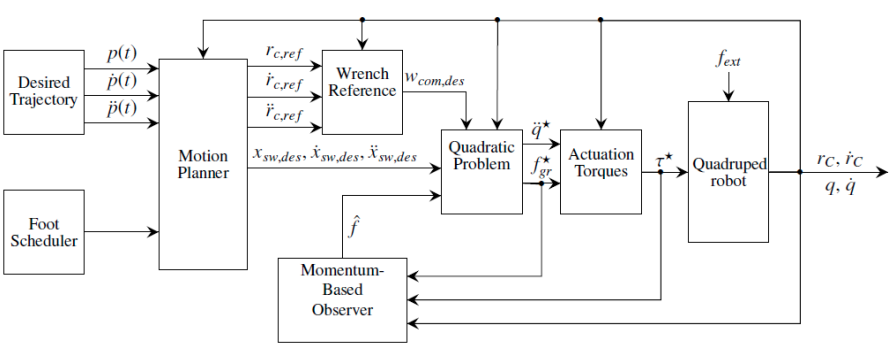
\includegraphics[width=0.75\linewidth]{Images/legged_robots_whole_body_controller.png}
    \caption{\textit{Whole-Body} Controller.}
    \label{fig:legged_whole_body_controller}
\end{figure}\\
This controller computes the desired joint accelerations $\ddot{q}_j^*$ and GRFs $f_{gr}^*$. Its inputs are:
\begin{itemize}
    \item A desired CoM's trajectory.
    \item The foot schedule, which is a function of the robot's gait, such as \textit{Trot} (cross legs move), \textit{Pace} (lateral legs work in coordination), \textit{Bound} (front and rear legs work in pair).
\end{itemize}
Then, a wrench-reference is computed and passed onto a Quadratic Solver, which solves a quadratic constrained problem. The constraints take care of dynamic consistency, non-sliding contacts, torque limits and swing legs tasks. Notice also the presence of a momentum-basd observer, which computes the external forces acting on the robot to compensate for them in the control. Let us look at the components more closely now.
\subsection{Motion Planner}
The motion planner takes as input a desired trajectory for the CoM and a foot schedule, giving as output the appropriate references; these are, generally speaking, regular curves, but due to numerical errors a drift can appear between the torso and feet movements, which is corrected at each planning step by the motion planner. The complete motion is divided into a \textit{Stance Phase} and a \textit{Swing Phase} by the foot-scheduler; then, desired path is composed by splines such that:
\begin{itemize}
    \item The initial state $p(0),\dot{p}(0),\ddot{p}(0)$ coincide with the center of the initial support polygon an the initial velocity and acceleration.
    \item The final state $p(t_f),\dot{p}(t_f),\ddot{p}(t_f)$ is set to be at the center of the polygon defined by the planned footholds, which is the polygon that would support the robot if it was to stop and stand at the end of the support polygon sequence.
\end{itemize}
Given the swing-phase duration $T_{sw}$ and the maximum step length, the motion planner computes a sequence of footholds.\\
During the stance-phase: the legs are all in contact with the ground, ensuring an intrinsic balance; the CoM reference $r_{c,ref}, \dot{r}_{c,ref}, \ddot{r}_{c,ref}$ can be computed as a 3-rd order spline that tracks the desired trajectory.\\
During the swing-phase: since at least one leg is swinging, both the CoM's trajectory and the swing feet motion have to be planned. Considering the reference $r_{c,ref}=[p_{c,ref}^{T},\eta_{c,ref}^{T}]^{T}$, the motion CoM's coordinates can be described by the $i$-th spline as:
\begin{gather*}
    p_{c,ref}^{(x)}=\alpha_{i3,x}t^{3}+\alpha_{i2,x}t^2+\alpha_{i1,x}t+\alpha_{i0,x}\\
    p_{c,ref}^{(y)}=\alpha_{i3,y}t^{3}+\alpha_{i2,y}t^2+\alpha_{i1,y}t+\alpha_{i0,y}\\
    p_{c,ref}^{(z)}=\alpha_{i3,z}t^{3}+\alpha_{i2,z}t^2+\alpha_{i1,z}t+\alpha_{i0,z}
\end{gather*}
Which can be restated as:
\begin{gather}
    \lambda(t)=
    \begin{bmatrix}
        t^3 & t^2 & t & 1
    \end{bmatrix},\\
    \alpha_{ik}=
    \begin{bmatrix}
        \alpha_{ik,x} & \alpha_{ik,y} & \alpha_{ik,z}    
    \end{bmatrix}^{T},\\
    \begin{bmatrix}
        \alpha_{i3} & \alpha_{i2} & \alpha_{i1} & \alpha_{i0}
    \end{bmatrix},\\
    T=
    \begin{bmatrix}
        \lambda(t) & 0 & 0\\
        0 & \lambda(t) & 0\\
        0 & 0 & \lambda(t)
    \end{bmatrix}, \\
    p_{c,ref}=T\alpha_i,\\
    \dot{p}_{c,ref}=\dot{T}\alpha_i,\\
    \ddot{p}_{c,ref}=\ddot{T}\alpha_i
\end{gather}
The motion planning algorithm is then formulated as a constrained nonlinear optimization problem which minimizes a generic cost function, with the spline stacked vector $\alpha_i$ as optimization variables. To ensure splines continuity, the following junction constraint is added:
\begin{gather}
    \begin{bmatrix}
        \lambda(t_{f_k})^{T} & -\lambda(0)^{T}\\
        \dot{\lambda}(t_{f_k})^{T} & -\dot{\lambda}(0)^{T}
    \end{bmatrix}
    \begin{bmatrix}
        \alpha_{k}^{x}\\
        \alpha_{k+1}^{x}
    \end{bmatrix}=0
\end{gather}
Where $t_{f_k}$ is the duration of spline $s_k$. Some constraints are also added to ensure stability, by constraining the ZMP (see definition n.\ref{legged_robotics_Center_of_pressure}) to stay inside the robot's support polygon. In particular, starting from the measured feet configuration, the motion plan is called and, using the planned feet positions, a sequence of support polygons and their duration is computed by using the contact schedule. 
\begin{figure}[htpb!]
    \centering
    \begin{minipage}{0.7\textwidth}
        \centering
        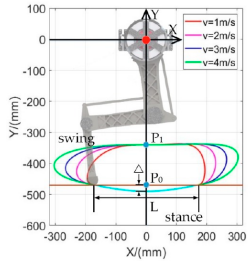
\includegraphics[width=0.7\linewidth]{Images/legged_swing_feet.png}
        \caption{Swing Feet splines.}
    \end{minipage}\hfill
    \begin{minipage}{0.3\textwidth}
        This can be achieved by imposing the constraint:
        \begin{gather*}
            ap_z^x+bp_z^y+c\geq 0
        \end{gather*}
        Where $a,b,c$ are the coefficients of the line passin through the vertices of an edge of the support polygon.\\
        Finally, the reference for the swing feet is computed using two splines, the former to lift the foot, the latter to lower it.
    \end{minipage}
\end{figure}
\subsection{Momentum Based Observer}
External forces are estimated to compensate for them inside the controller; in order to take into account the disturbances acting on both stance and swing legs, the observer considers the momentum of all the legs, given by:
\begin{equation}
    \dot{\rho}=\bar{C}_{2}^{T}\dot{q}_{j}+\bar{J}_{st,j}^{T}f_{gr}+\tau+\bar{J}_{j}^{T}f_{ext}
\end{equation}
By defining:
\begin{itemize}
    \item $\hat{F}=\bar{J}_{j}^{T}\in\mathbb{R}^{n_j}$, which represents the estimated joint torques corresponding to the resultant force at the legs' tips.
    \item $F_{ext}=\bar{J}_{j}^{T}f_{ext}\in\mathbb{R}^{n_j}$, which represents the effect at the joint torques of the resultant force at the legs' tips.
\end{itemize}
The estimator can be designed to achieve a linear relationship between the estimated external forces and the real ones in the Laplace domain as:
\begin{definition}\label{legged_estimator}
    \textit{Legged Robot Momentum-Based Observer}: The Momentum-Based Observer used in the Whole-Body controller is designed as:
    \begin{gather}\label{legged_estimator_eq}
        \hat{F}=G(s)F_{ext}\\
        \alpha(t)=\bar{C}_{2}^{T}\dot{q}_{j}+\tau+\bar{J}_{st,j}^{T}f_{gr}\\
        \gamma_1=K_1\left[\rho(t)-\int_{0}^{t}\left(\hat{F}(\sigma)+\alpha(\sigma)\right)d\sigma\right]\\
        \gamma_i=K_i\int_{0}^{t}{\left(-\hat{F}(\sigma)+\gamma_{i-1}(\sigma)\right)d\sigma}, \quad i=2,\dots,r
    \end{gather}
    Where:
    \begin{itemize}
        \item $r$ is the desired estimator's degree.
        \item $\hat{F}=\gamma_r$.
        \item $K_i\in\mathbb{R}^{n_j\times n_j}$ are positive definite matrices.
    \end{itemize}
\end{definition}
\subsection{Quadratic Problem}
The desired acceleration and the desired ground reaction forces are obtained through a quadratic problem, formally defined as:
\begin{definition}\label{legged_quadratic_problem}
    \textit{(Legged Robot's Quadratic Problem for Motion Planning)}: The QP used in the Whole-Body Controller is formally defined as:
    \begin{gather*}
        \zeta=
        \begin{bmatrix}
            \ddot{r}_{c}^{T} & \ddot{q}_{j}^{T} & f_{gr}^{T}
        \end{bmatrix}\in\mathbb{R}^{n_b+n_j+3n_{st}},\\
        r_c=
        \begin{bmatrix}
            p_c^T & \eta_c^T
        \end{bmatrix}^T,\\
        \min_{\zeta} f(\zeta)\\
        \text{subject to:}\\
        A\zeta=b\\
        D\zeta\leq c\\
    \end{gather*}
\end{definition}
The cost function aims at tracking the CoM's reference; to this end, consider the first $n_b$ equations of the centroidal dynamics defined in eq:\ref{legged_Centroidal_Dynamics_Model}:
\begin{gather*}
    M_{CoM}(q)\ddot{r}_c+mg=\bar{J}_{st,c}^{T}f_{gr}+\bar{J}_{c}^{T}f_{ext}=W_{CoM},\\
    M_{CoM}=
    \begin{bmatrix}
        mI_3 & 0\\
        0 & M_{11}
    \end{bmatrix}
\end{gather*}
Where $W_{CoM}\in\mathbb{R}^{6}$ is the wrench at the robot's CoM. To get bounded interaction forces a suitable compliant behavior has to be ensured for this kind of robot; this is achieved by using a compliant approach.
\begin{definition}\label{legged_compliant_reference}
    \textit{(Compliant Reference approach for a legged robot)}: 
    \begin{gather}\label{legged_compliant_reference_eq}
        W_{CoM,des}=-K_p\left(r_c-r_{c,ref}\right)-K_d\left(\dot{r}_{c}-\dot{r}_{c,ref}\right)+mg+M_{CoM}(q)\ddot{r}_{c,ref},\\
        K_p,K_d\in\mathbb{R}^{3\times 3}
    \end{gather}
    Where the terms $-K_p\left(r_c-r_{c,ref}\right)-K_d\left(\dot{r}_{c}-\dot{r}_{c,ref}\right)$ represent a Cartesian Impedance term controlled by the positive definite matrices $K_p,K_d$. Then, the desired cost function for the QP optimization problem can be defined to be:
    \begin{gather}\label{legged_compliant_cost}
        f(\zeta)=\|\bar{J}_{st,c}^{T}\Sigma\zeta+\bar{J}_{st,c}^{T}\hat{f}_{st}-W_{CoM,des}\|+\|\zeta\|
    \end{gather}
    Where $\Sigma\in\mathbb{R}^{n_b+n_j+3_{st}}$ is a matrix selecting the last $3n_{st}$ elements of $\zeta$, the GRFs.
\end{definition}
Finally, the constraints can be introduced. These are:
\begin{itemize}
    \item \textit{(Dynamical consistency constraints:)} 
    The centroidal dynamics is imposed under the assumption of perfect compensation (or absence) of external disturbances; the constraint can then be expressed as:
    \begin{gather}\label{legged_robot_dynamic_consistency_constraint}
        \begin{bmatrix}
            M_{CoM}(q) & 0_{n_b\times n_j} & -\bar{J}_{st,c}^{T}
        \end{bmatrix}\zeta=-mg
    \end{gather}
    \item \textit{(Non-sliding contact constraints:)}
    To avoid slipping, the Ground Reaction Forces at the feet contact points have to be constrained inside a friction cone. Define $\bar{n}_{i}$ to be the normal vector at the contact point with the ground for the $i$-th foot and $\bar{l}_{1,i},\bar{l}_{2,i}$ the tangential vectors at the same point; then, for each foot:
    \begin{gather*}
        \begin{cases}
            (\bar{l}_{1,i}-\mu\bar{n}_i)^{T}f_{gr,i}\leq0\\ 
            -(\bar{l}_{1,i}+\mu\bar{n}_i)^{T}f_{gr,i}\leq0\\
            (\bar{l}_{2,i}-\mu\bar{n}_i)^{T}f_{gr,i}\leq0\\
            -(\bar{l}_{2,i}+\mu\bar{n}_i)^{T}f_{gr,i}\leq0 
        \end{cases}
    \end{gather*}
    This can also be written in matrix form with respect to the control variables $\zeta$:
    \begin{gather}\label{legged_robot_non_sliding_constraint}
        \begin{bmatrix}
            0_{4\cdot n_{st}\times n_b} & 0_{4\cdot n_{st}\times n_j} & D_{fr}
        \end{bmatrix}\zeta\leq 0_{4\cdot n_{st}}
    \end{gather}
    Where $D_{fr}=diag(D_1,D_2,\dots,D_{n_{st}})$, with:
    \begin{gather*}
        D_i=
        \begin{bmatrix}
            (\bar{l}_{1,i}-\mu\bar{n}_i)^{T}f_{gr,i}\leq0\\ 
            -(\bar{l}_{1,i}+\mu\bar{n}_i)^{T}f_{gr,i}\leq0\\
            (\bar{l}_{2,i}-\mu\bar{n}_i)^{T}f_{gr,i}\leq0\\
            -(\bar{l}_{2,i}+\mu\bar{n}_i)^{T}f_{gr,i}\leq0\\
        \end{bmatrix}
    \end{gather*}
    \item \textit{(Torque limits constraints):}
    Focusing on the motion equations regarding the robot’s legs, the constraints about limited torques can be expressed as follow:
    \begin{gather*}
        \tau_{min}-\bar{C}_2\dot{q}_j\leq M_{22}\ddot{q}_j-\bar{J}_{st,j}^{T}f_{gr}\leq \tau_{max}-\bar{C}_2\dot{q}_j
    \end{gather*}
    Which can be expressed using the control variables as:
    \begin{gather}\label{legged_robot_torque_limits_constraints}
        \begin{cases}
            \begin{bmatrix}
                0_{n_j\times n_b}& M_{22} & -\bar{J}_{st,j}^{T}
            \end{bmatrix}\zeta\leq \tau_{max}-\bar{C}_{2}\dot{q}_j\\
            \begin{bmatrix}
                0_{n_j\times n_b}& -M_{22} & \bar{J}_{st,j}^{T}
            \end{bmatrix}\zeta\leq -\tau_{min}+\bar{C}_{2}\dot{q}_j\\
        \end{cases}
    \end{gather}
    \item \textit{(Swing leg task constraints)}:
    Necessary for the swing feet to follow the assigned trajectory; since the reference for the swing feet can be written as:
    \begin{gather*}
        \ddot{x}_{sw,cmd}=\ddot{x}_{sw,des}+K_{d,w}(\dot{x}_{sw,des}-\dot{x}_{sw})+\\+K_{p,sw}(x_{sw,des}-x_{sw})-J_{sw}M_{x}^{-1}N_{c}J_{sw}^{T}\hat{f}_{sw}
    \end{gather*}
    Where $N_c$ is the dynamically consistent support null-space matrix defined in eq:\ref{legged_robotics_dynamically_consistent_projection_operator} and $x_{sw}$ is the position of the swing feet. Then, to follow the trajectory, the following equality constraint should be imposed:
    \begin{gather*}
        \bar{J}_{sw,c}\ddot{r}_{c}+\dot{\bar{J}}_{sw,c}\dot{r}_{c}+\bar{J}_{sw,j}\dot{q}_{j}=\ddot{x}_{sw,cmd}
    \end{gather*}
    However, these constraints are often softened by adding slack variables $\gamma\in\mathbb{R}^{3n_{sw}}$. The new constraints are given as a function of the expanded control vector:
    \begin{gather*}
        \zeta'=
        \begin{bmatrix}
            \ddot{r}_c^T&\ddot{q}_j^T&f_{gr}^T&\gamma^T
        \end{bmatrix}^T
    \end{gather*}
    \begin{gather}\label{legged_robotics_swing_leg_task_constraints}
        \begin{cases}
            \begin{bmatrix}
                \bar{J}_{sw,c}&\bar{J}_{sw,j}& 0_{3n_{sw}\times 3n_{st}} & I_{3n_{sw}\times 3n_{sw}}
            \end{bmatrix}\zeta'\leq \ddot{x}_{sw,cmd}-\dot{\bar{J}}_{sw,c}\dot{r}_{c}-\dot{\bar{J}}_{sw,j}\dot{q}_j\\
            \begin{bmatrix}
                -\bar{J}_{sw,c}&-\bar{J}_{sw,j}& 0_{3n_{sw}\times 3n_{st}} & -I_{3n_{sw}\times 3n_{sw}}
            \end{bmatrix}\zeta'\leq -\ddot{x}_{sw,cmd}+\dot{\bar{J}}_{sw,c}\dot{r}_{c}+\dot{\bar{J}}_{sw,j}\dot{q}_j
        \end{cases}
    \end{gather}
    Taking into account the constraints, the quadratic problem is fully characterized by the matrices:
    \begin{gather}\label{legged_robot_QP_matrices}
        A=
        \begin{bmatrix}
            M_{CoM}(q) & 0_{n_b\times n_j} & -\bar{J}_{st,c}^T & 0_{n_b\times 3n_{sw}}\\
            \bar{J}_{st,c} & \bar{J}_{st,j} & 0_{3n_{st}\times 3n_{st}} & 0_{3n_{st}\times 3n_{sw}}
        \end{bmatrix},\\
        b=
        \begin{bmatrix}
            -mg\\
            -\dot{\bar{J}}_{st,c}\dot{r}_{c}-\dot{\bar{J}}_{st,j}\dot{q}_j
        \end{bmatrix},\\
        D=
        \begin{bmatrix}
            0_{3n_{st\times 6}} & 0_{4n_{st\times n_{j}}} & D_{fr} & 0_{4n_{st}\times 3n_{sw}}\\
            0_{n_j\times n_b} & M_{22} & -\bar{J}_{st,j}^{T} & 0_{n_j\times 3n_{sw}}\\
            0_{n_j\times n_b} & -M_{22} & \bar{J}_{st,j}^{T} & 0_{n_j\times 3n_{sw}}\\
            \bar{J}_{sw,c} & \bar{J}_{sw,j} & 0_{3n_{sw}\times 3n_{st}} & I_{3n_{sw}\times 3n_{sw}}\\
            -\bar{J}_{sw,c} & -\bar{J}_{sw,j} & 0_{3n_{sw}\times 3n_{st}} & I_{3n_{sw}\times 3n_{sw}}
        \end{bmatrix}, \\
        c=
        \begin{bmatrix}
            0_{4n_{st}}\\
            \tau_{max}-\bar{C}_{2}\dot{q}_{j}\\
            -\tau_{min}+\bar{C}_{2}\dot{q}_{j}\\
            \ddot{x}_{sw,cmd}-\dot{\bar{J}}_{sw,c}\dot{r}_{c}-\dot{\bar{J}}_{sw,j}\dot{q}_{j}\\
            -\ddot{x}_{sw,cmd}+\dot{\bar{J}}_{sw,c}\dot{r}_{c}+\dot{\bar{J}}_{sw,j}\dot{q}_{j}\\
        \end{bmatrix}
    \end{gather}
\end{itemize}

 \newpage             
 \chapter{Appendix}
                \section{Probability and State Estimation}
                    \subsection{Probability Primer}
                        The study of the Theory of Probability could be described as the study of "uncertain outcomes" and it is easily one of the most counterintuitive fields of mathematics. It is also enormous. Here, only the very basics will be introduced, just enough to better understand the following discussions on \textit{Probabilistic Robotics} and \textit{Filters}. The following discussion will be pretty mathematically heavy and precise, but there will also be some colloquial paraphrasing of the introduced notions.
                        \subsubsection{Measurable Spaces and Probability Spaces}
                            \begin{definition}\label{sigma_algebra}
                                Let $\mathcal{F}$ be a non-empty family of subsets of a set $\Omega$. $\mathcal{F}$ is a $\sigma$\textit{-algebra} over $\Omega$ if and only if:
                                \begin{itemize}
                                    \item If $A \in \mathcal{F}$, then $A^c:=\Omega/A\in\mathcal{F}$: the set $\mathcal{F}$ is closed under taking complements.
                                    \item The countable \footnote{A set $X$ is \textit{countable} if and only if there exists a surjective mapping $f:\mathbb{N}\rightarrow X$} union of elements of $\mathcal{F}$ is still in $\mathcal{F}$: the set $\mathcal{F}$ is closed under taking the countable union of its elements.
                                \end{itemize}
                            \end{definition}
                            It is an easy exercise that a $\sigma$-algebra is also closed under countable intersections. Another two definitions, then the "why should we care" will be explained:
                            \begin{definition}\label{measurable_space}
                                A \textit{measurable space} is the couple $\left(\mathcal{F},\Omega\right)$ such that:
                                \begin{itemize}
                                    \item $\Omega\neq\emptyset$.
                                    \item $\mathcal{F}$ is a $\sigma$-algebra on $\Omega$.
                                \end{itemize}
                            \end{definition}
                            \begin{definition}\label{measure}
                                A \textit{measure} over the measurable space $\left(\mathcal{F},\Omega\right)$ is a function:
                                \begin{equation*}
                                    \mu:\mathcal{F} \rightarrow [0,+\infty]
                                \end{equation*}
                                Such that:
                                \begin{itemize}
                                    \item $\mu(\emptyset)=0$.
                                    \item $\mu$ is $\sigma$\textit{-additive} over $\mathcal{F}$, meaning that:
                                    \begin{equation*}
                                        \mu\left(\bigcup_{n=1}^{\infty}A_n\right)=\sum_{n=1}^{\infty}\mu(A_n)
                                    \end{equation*}
                                \end{itemize}
                            \end{definition}
                            The definition of $\sigma$-algebra is necessary in this context to represent \textit{events}: these are the measured result of a probabilistic experiment. However, events could also be composed of single \textit{outcomes}, which are represented by the elements of $\Omega$. As an example, in the experiment:
                            \begin{equation*}
                                \textit{If a dice is thrown, what is the probability of obtaining 5 as a result?}
                            \end{equation*}
                            The event $A$=\textit{"The result of the throw is 5"}$\in\mathcal{F}$ coincides with the outcome:
                            \[\omega_1=\textit{"the throw results in 5"}\in\Omega\]
                            However, it is equally plausible to ask:
                            \begin{equation*}
                                \textit{If a dice is thrown, what is the probability of obtaining a result smaller than 5?}
                            \end{equation*}
                            The event:
                            \[A=\textit{"The result of the throw is less than 5"}\in\mathcal{F}\]
                            Would actually be composed of more than one outcome: $A=\{\omega_1,\omega_2,\omega_3,\omega_4\}$. Then, the need for the definition of a measure is easily understood: it measures exactly the probability of the event passed to it as an argument. From these observations, the following definition is natural.
                            \begin{definition}
                                A measurable space $(\mathcal{F},\Omega,P)$ with $P(\Omega)=1$ is called a \textit{Probability Space}. The set $\Omega$ is called the \textit{set of outcomes}, $\mathcal{F}$ is the $\sigma$-algebra of \textit{events} and $P(A)$ is the \textit{probability} of the event $A\in\mathcal{F}$.   
                            \end{definition}
                            The requirement $P(\Omega)=1$ is obvious: it just states that \textit{some event} will surely manifest. Notice that the event $A=\Omega/\Omega=\emptyset\in\mathcal{F}$ is legal by the definition of $\sigma$-algebra, meaning that an event doesn't necessarily mean that \textit{something} will happen. 
                    \subsection{State Estimation: Filters}
                        One of the many differences between static robots and moving ones is the increased difficulty in state estimation. Indeed, an industrial manipulator has the possibility of using fixed landmarks and \textit{proprioceptive} sensors to estimate its state; meanwhile, for a mobile robot, this is not possible with high enough accuracy, due to the (often) dynamic environment and the additional noise afflicting the on the onboard sensors. The problem of \textit{State Estimation} is then solved by \textit{probabilistic} methods, in particular by making use of \textit{filters}.\\
                        Although a full discussion on filters would probably take an entire book, it is instructive to at least mention some of them and their differentiation. Filters can be divided into two main categories:
                        \begin{itemize}
                            \item \textit{Parametric Filters}: these assume a predefined formulation of the probability distribution for the state (probabilistic) variable $x$; often a Uniform Gaussian Distribution is assumed. These filters are capable of estimating the \textit{parameters} which describe the PDF\footnote{\textit{Probability Distribution Function}}. This kind of filters are very computationally efficient, however greatly sensitive to the system high nonlinearity and to multimodal distribution.
                            \item \textit{Non-Parametric Filters}: these don't assume \textit{any} kind of formulation for the PDF, but represent it by taking a set of samples, called \textit{particles}, and making computation based on them. These filters are called \textit{Particle Filters}. Although computationally heavy, they can represent a wide variety of PDFs, even multimodal ones.
                        \end{itemize}
                        \subsubsection{Parametric Filters}
                            There are plenty of types of parametric filters, but arguably the most famous is the \textit{Kalman Filter}. The Kalman Filter is a \textit{linear} (it assumes that the analyzed system's dynamics is linear) \textit{Gaussian} filter, i.e. it assumes that the state transition probability is a Gaussian PDF:
                            \begin{equation}\label{Gaussian_PDF}
                                p(x_t\mid u_t,x_{t-1})=\det(2\pi R_t)^{-1/2}exp\left\{-\frac{1}{2}\left(x_t-A_tx_{t-1}-B_{t}u_{t}\right)^{T}R_t^{-1}\left(x_t-A_tx_{t-1}-B_{t}u_{t}\right)\right\}
                            \end{equation}
                            Where:
                            \begin{itemize}
                                \item $x_t=A_tx_{t-1}+B_tu_t+\epsilon_t$ is the perturbed linear dynamic model of the system ($\epsilon_t$ is Gaussian noise).
                                \item $R_t$
                            \end{itemize}


                            
                \section{Motion Planning}
                    \subsection{Introduction}
                        A fundamental need in robotics is to have algorithms that convert high-level specifications of tasks from humans into low-level descriptions of how to move in an environment which can be either dynamic or static. A classic example of this is the \textit{Piano Mover's Problem}.
                        \begin{figure}[h!]
                            \centering
                            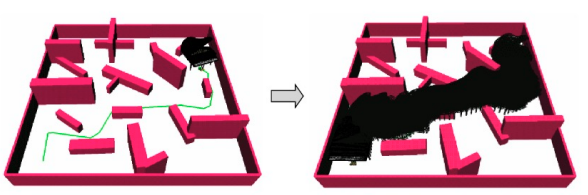
\includegraphics[width=0.8\linewidth]{Images/image22.png}
                            \caption{3D Piano Mover's Problem}
                            \label{fig:Piano_Movers_Problem}
                        \end{figure}
                        This need is expressed by the \textit{Motion Planning Problem}:
                        \begin{definition}\label{Motion_Planning_Problem}
                            Given the initial $q_0$ desired $q_d$ poses of a robot $\mathcal{B}$ in the environment $\mathcal{W}=\mathbb{R}^n$,$n\in\{2,3\}$, the problem of \textit{ Motion Planning} is to find, if it exists, a path that drives the robot between the two poses without any contact or collision with obstacles $\left\{\mathcal{O_{i}}\right\}_{i=1}^{p}$.
                        \end{definition}
                        Planning can be either done in \textit{online} during execution of the tasks, or \textit{offline}. Offline planning is obviously only really feasible if the environment does not change, i.e. it is \textit{static}. \\
                        Some assumptions are introduced:
                        \begin{itemize}
                            \item The positions of the obstacles $\{\mathcal{O_i}\}_{i=1}^{p}$ are known and fixed, at least for offline planning. Each set $\mathcal{O}_i$ is closed and contains its boundary. Notice that it is not necessary for the obstacles to be limited subsets of $\mathcal{W}$.
                            \item The robot $\mathcal{B}$ can move instantaneously everywhere (although this assumption will be relaxed later).
                        \end{itemize}
                    \subsection{Distance, Obstacles and \textit{Free Configuration Space}}
                        It is known that, on an Euclidean Space there always exists a metric (\textit{Euclidean Metric}) which in turn establishes a norm. However, the Configuration Space is not necessarily an Euclidean Space, which immediately begs the question of how to measure distances. Intuition suggests that the distance between two robot configurations, $q_1,q_2$, should be zero if the space occupied by the robot $\mathcal{B}$ in those configurations is the same; let:
                        \begin{itemize}
                            \item $\mathcal{B(q)}\subseteq\mathcal{W}$ be the subset of the environment occupied by the robot in the configuration $q$.
                            \item Let $p(q)$ be the position in $\mathcal{W}$ of a robot's point, taken as a reference. This naturally implies that $p\in\mathcal{B}$.
                        \end{itemize}
                        Then, the \textit{uniform metric} is adopted:
                        \begin{equation}\label{uniform_C_space_norm}
                            d(q_1,q_2)=\max_{p\in\mathcal{B}} ||p(q_1)-p(q_2)||
                        \end{equation}
                        Next, it is necessary to map an obstacle from $\mathcal{W}$ to the $\mathcal{C}$-space. This is done by introducing the \textit{C-obstacle}.
                        \begin{definition}
                            Let $\mathcal{O}_{i}\in\mathcal{W}$, $i \in \{1,\dots,p\}$, be an obstacle in $\mathcal{W}$. Then, the image of the obstacle in the configuration space is defined as:
                            \begin{equation}\label{C_obstacle_image}
                                \mathcal{CO}_{i}=\left\{q \in \mathcal{C}: \mathcal{B}(q) \cap \mathcal{O}_{i} \neq \emptyset \right\}
                            \end{equation}
                            This is the set of configurations that cause a collision with the $i$-th obstacle. Then, the union:
                            \begin{equation}\label{C_osbstacle}
                                \mathcal{CO}=\bigcup_{i=1}^{p}\mathcal{CO}_{i}
                            \end{equation}
                            It is called $\mathcal{C}$\textit{- obstacle region} and is the set of configurations that cause a collision with at least one obstacle.
                        \end{definition}
                        The complement of the $\mathcal{C}$-space with respect to $\mathcal{CO}$ gives:
                        \begin{definition}\label{free_configuration_space}
                            The \textit{Free Configuration Space} $\mathcal{C}_{free}$:
                            \begin{equation}\label{free_configuration_eq}
                                \mathcal{C}_{free}=\mathcal{C}/\mathcal{CO}
                            \end{equation}
                            Is the set of configurations which do not cause collisions with any obstacle. A \textit{free-path} is a path completely contained in $\mathcal{C}_{free}$
                        \end{definition}
                        The computation of these spaces is computationally heavy, if not outright intractable. However, it is possible to approximate them by \textit{sampling} the space and adopting \textit{Grid Representations}.
                    \subsection{Grid-Based Mapping}
                        The approximation of the $\mathcal{C}$-space is almost mandatory in real applications, as is easily understood. A structure used to represent the approximation of the $\mathcal{C}_{free}$ is called a \textit{Roadmap}. The most basic procedure adopted for an approximation-based Motion Planner could be:
                        \begin{itemize}
                            \item Approximate $\mathcal{C}_{free}$.
                            \item Find a path connecting $q_i$ to $q_f$, if it exists.
                            \item At each planner iteration, a sampled model configuration is chosen and checked if it leads to collisions with obstacles. if there are, the sample is discarded from $\mathcal{C}_{free}$; if there is no collision, the sample is saved in the current Roadmap.
                        \end{itemize}
                        \begin{figure}[htbp!]
                            \begin{minipage}{0.6\textwidth}
                                    \centering
                                    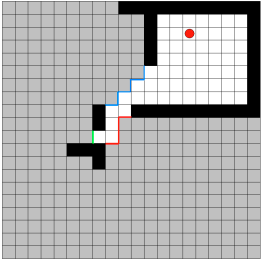
\includegraphics[width=0.6\linewidth]{Images/image23.png}
                                    \caption{Grid-Map}
                                    \label{fig:grid_map}
                            \end{minipage}\hfill
                            \begin{minipage}{0.4\textwidth}
                                A \textit{Grid-based} approximation is based on a discretization of the configuration space as a set of occupied and free cells; this approach can also be used in a $3D$ map. Increasing the resolution of the cells help to speed up the planning process, however giving rise to worse paths. This approach also has some criticalities which must be addressed in the design of the Motion Planner. In particular, the choice of an appropriate data structure is of great importance; a chosen data structure should be easy to read, maintain in memory and visualize for a human operator.
                            \end{minipage} 
                        \end{figure}
                        \subsubsection{Probabilistic Roadmap Method: \textit{PRM}}
                            Assuming to have successfully generated a grid-map, it is then time to plan a motion. The most n\"{a}ive approach would be to (uniformly) randomly generate a sample configuration $q_s\in \mathcal{C}$ and check its feasibility, either by a direct representation of $\mathcal{CO}$ or by kinematics arguments. \\
                            The procedure at $i$-th iteration would look like:
                            \begin{itemize}
                                \item Generate the random sample $q_s^{(i)}$.
                                \begin{itemize}
                                    \item If $q_s^{(i)}$ generates a collision, it is discarded.
                                    \item if $q_s^{(i)}$ does not generate a collision, it is added to the Roadmap.
                                \end{itemize}
                                \item The \textit{Local Planner} checks for the nearest feasible configuration $q_{near}^{(i)}$, based on the used metric on $\mathcal{C}$. A path is searched to link $q_s^{(i)}$ and $q_{near}^{(i)}$. A common choice of such a path would be a rectilinear path, which is sampled and checked for collision.
                            \end{itemize}
                            Once the iterations stop (due to some criterion), a representation of $\mathcal{C}_{free}$ is obtained. The next step is to find paths that connect $q_i$, $q_f$ completely contained into $\mathcal{C}_{free}$. Then:
                            \begin{itemize}
                                \item The Local Planner links $q_s$ and $q_f$ to the Roadmap.
                                \item A search algorithm is used to find the path connecting $q_s,q_f$ along the Roadmap.
                            \end{itemize}
                            Notice that the PRM is probabilistic, which means that if a solution that connects the initial and desired configurations does not exist, the algorithm keeps on searching without ever stopping. However, it has the advantage of not requiring an explicit description of $\mathcal{CO}$, which is a big deal. 
                        \subsubsection{Artifical Potential Methods}
                            Although powerful, PRM has been used under the assumption of a static environment. However, it often the case that robots have to execute tasks in a \textit{dynamic} environment. To this end, the method of \textit{Artificial Potential} is introduced; its main objective is not to reconstruct $\mathcal{C}_{free}$, but only to reach the desired configuration $q_f$.\\
                            The method exploits the superposition of two terms:
                            \begin{itemize}
                                \item An \textit{attractive} potential term, which guides the robot:
                                    \begin{itemize}
                                        \item A first choice could be:
                                            \begin{equation}\label{attractive_potentia_1}
                                                U_a(q)=\frac{1}{2}k_ae^{T}(q)e(q)=\frac{1}{2}k_a ||e(q)||^2
                                            \end{equation}
                                            Where $k_a>0, e(q)=q_f-q$. The resulting force is:
                                            \begin{equation*}
                                                f_a(q)=-\nabla U_a(q)=k_a e(q)
                                            \end{equation*}
                                        \item Another choice could be:
                                            \begin{equation}\label{attractive_potential_2}
                                                U_b(q)=k_a||e(q)||
                                            \end{equation}
                                            Where $k_a>0,e(q)=q_f-q$. The resulting force is:
                                            \begin{equation*}
                                                f_b(q)=-\nabla U_b(q)=k_a \frac{e(q)}{||e(q)||}
                                            \end{equation*}
                                            However note that this is not defined at the target configuration and the robot converges more slowly to the target than with the other choice. However, this force doesn't go to infinity for large errors $e(q)$, so it is useful for starting configurations.
                                    \end{itemize}
                                \item A \textit{repulsive} potential term, which pushes the robot away from the $\mathcal{CO}-$obstacle region. Assuming $\mathcal{CO}$ to be convex or partitioned into convex regions $\mathcal{CO}_i$, then each region's associated repulsive potential is:
                                \begin{equation}\label{repulsive_potential}
                                    U_{r,i}(q)=
                                    \begin{cases}
                                        \frac{k_{r,i}}{\gamma} \left[\frac{1}{\eta_i(q)}-\frac{1}{\eta_{o,i}(q)}\right]^\gamma \text{, } \eta_i(q)\leq \eta_{o,i} \\
                                        0 \text{, } \eta_{i}(q)>\eta_{o,i}
                                    \end{cases}
                                \end{equation}
                                Where: 
                                \begin{itemize}
                                    \item $k_{r,i}>0$ is a positive gain.
                                    \item $\eta_i(q)=\min_{q'\in \mathcal{CO}_{i}}||q-q'||$.
                                    \item $\eta_{o,i}$ is the obstacle's \textit{range of influence}.
                                    \item $\gamma \in \{2,3\}$.
                                \end{itemize}
                                Then, the induced force is:
                                \begin{gather*}
                                    f_{r,i}(q)=- \nabla U_{r,i}(q)= \\
                                    \begin{cases}
                                        \frac{k_{r,i}}{\eta_{i}^{2}(q)} \left[\frac{1}{\eta_{i}(q)}-\frac{1}{\eta_{o,i}}\right]^{\gamma-1} \nabla\eta_i(q), \text{ }\eta_i(q) \leq \eta_{o,i} \\
                                        0, \text{ } \eta_i(q)>\eta_{o,i}
                                    \end{cases}
                                \end{gather*}
                                The convexity hypothesis was necessary for $\nabla \eta_i(q)$ to be analytically computed.
                            \end{itemize}
                            The total potential and force are then the sum of all individual potentials and forces. Although the name suggests it, the total force is \textit{not} necessarily applied as an actual force on the robot, in fact there are different interpretations:
                            \begin{itemize}
                                \item $f_t(q)=\tau$: The total force is seen as the vector of generalized forces (force plus torques) that induce a motion of the robot according to its dynamic model. If the planning is online, the total force is taken as the input to the robot; otherwise, it generates smooth trajectories since the reactions of the robot are filtered by the robot dynamics.
                                \item $f_t(q)=\ddot{q}$: The total force is seen as the acceleration moving the robot, that is considered as a point mass. In the case of online planning, a solution of the inverse dynamics problem or an online $2$° order kinematic control scheme are required. 
                                \item $f_t(q)=\dot{q}$: The total force is seen as the velocity vector moving the robot, that is considered from a kinematic viewpoint only. This is the most common choice, with the unique advantage of ensuring the reachability of the final configuration $q_f$ with zero velocity (meanwhile the other control schemes require an additional damping term).
                            \end{itemize}
                            Notice that Artificial Potential Methods suffer from a drawback: local minima. These can cause the robot to stall in configurations different from the desired ones:
                            \begin{gather*}
                                \begin{cases}
                                    f_t(\bar{q})=0\\
                                    U_t(\bar{q})>0
                                \end{cases} \text{ with }\bar{q}\neq q_g
                            \end{gather*}
                            These are generally addressed by heuristic methods.
            \newpage
                \section{Lyapunov Theory}
                    \subsection{LaSalle's Invariant Set Theorem}
                    \subsection{Barbalat's Lemma}
                        Lyapunov's Theorem establishes that given a Lyapunov Function whose derivative is negative definite, at least in a local neighbor of the origin, then the origin is an asymptotically stable equilibrium. However, finding a Lyapunov Function is a laborious task, especially with the required negative-defineteness on its Lie Derivative. In the case of autonomous systems, i.e. systems with no explicit time dependence, it is possible to apply LaSalle's Invariant Set Theorem to prove asymptotical stability of the equilibrium, given a \textit{semi}-negative definite Lie Derivative of the Lyapunov Function; unfortunately, this does not work with \textit{non-autonomous} systems, which are of interest in the context of mobile robots. \\
                        This problem is addressed by another fundamental result in stability theory: \textit{Barbalat's Lemma}. There are a few formulations of this theorem, but the most used one is the following:
                        \begin{definition}
                            (\textit{Barbalat's Lemma in scalar form} ($1$)): Let $f(t): \mathbb{R}\rightarrow\mathbb{R}$ have a finite limit for $t\rightarrow\infty$ and $\dot{f}(t)$ uniformly continuous; then, $\dot{f}(t)\rightarrow0$ for $t\rightarrow\infty$. 
                        \end{definition}
                        Notice that $|\ddot{f}(t)|<\infty$ is a sufficient condition for $\dot{f}(t)$ to be uniformly continuous. There is also an alternative version:
                        \begin{definition}
                            (\textit{Barbalat's Lemma in scalar form} ($2$)): Let $p\in[1,\infty)$, $q\in(1,\infty]$. If $f\in\mathcal{L}^{p}(0,\infty)$
                            \footnote{Remember that a function $f$ is an element of $\mathcal{L}^{p}(a,b)$ if and only if: 
                            \begin{equation*}
                                \left[\int_{a}^{b}{|f(x)|^{p}dx}\right]^{p}<\infty
                            \end{equation*}
                            } 
                            and $\dot{f}\in \mathcal{L}^{q}(0,\infty)$, then $f(t)\rightarrow0$ as $t\rightarrow\infty$.
                        \end{definition}
                        In vector form the theorem becomes:
                        \begin{definition}
                            (\textit{Barbalat's Lemma in vector form}): Let $f(t): \mathbb{R}^{n}\rightarrow\mathbb{R}^{m}$ be uniformly continuous over the Banach Space $(E,||\cdot ||)$\footnote{Remember that a Banach Space is an normed space $(E,||\cdot ||)$ closed under Cauchy sequences.} and assume:
                            \begin{equation*}
                                \lim_{t\rightarrow \infty}\left|\int_{0}^{t}{f(\tau)d\tau}\right| <\infty
                            \end{equation*}
                            Then, $f(t)\rightarrow0$ as $t\rightarrow\infty$.
                        \end{definition}
            \newpage
                \section{Mathematical Appendix}
                    \subsection{Vector Fields and Operators}
                        \begin{definition}
                        (\textit{Vector Field}): Given a subset $S\subseteq \mathbb{R}^{n}$, a \textit{vector field} is represented by a vector-valued function $V: S \rightarrow \mathbb{R}^{n}$ in standard Cartesian Coordinates. 
                        \end{definition}
                        If each component of $V$ is continuous, then $V$ is a continuous vector field. If each component is \textit{smooth} (meaning $C^\infty$), then so is the vector field. Geometrically speaking, a vector field assigns a vector to each point in space.
                        Similarly, a \textit{Co-vector Field} is a vector field acting on co-vectors. Since $f$ maps onto $\mathbb{R}^n$, it is possible to use the standard inner-product:
                        \[\langle w^*,v\rangle=\sum_{j}w_{j}^{*}v_j\]
                        There are other useful operators that will be needed from now on:
                        \begin{itemize}
                            \item \textit{Gradient}: This one should also be already familiar; assume $\lambda:\mathbb{R}^n \rightarrow \mathbb{R}$, the \textit{Gradient} of $\lambda$ is defined as:
                            \begin{equation}\label{Gradient}
                                d\lambda(x)=\left[\frac{\partial\lambda}{\partial x_1}, \dots,\frac{\partial\lambda}{\partial x_n}\right]
                            \end{equation}
                            \item \textit{Lie Derivative}: Let $f$ be a vector field and $\lambda$ a real-valued scalar function, then the \textit{Lie Derivative} is defined as:
                            \begin{equation}\label{Lie_Derivative}
                                L_{f}\lambda=\langle\lambda(x),f(x)\rangle=\frac{\partial\lambda}{\partial x}\cdot f(x)               
                            \end{equation}
                            Geometrically, it expresses how the vector field is oriented with respect to the gradient of the scalar field.
                            \item \textit{Lie Bracket}: Let $f,g$ be two vector fields; then the \textit{Lie Bracket} is defined as:                         \begin{equation}\label{Lie_Bracket}                                    \left[f(x),g(x)\right]=\frac{\partial g}{\partial x} f- \frac{\partial f}{\partial x} g 
                            \end{equation}
                            
                        \end{itemize}
                    \subsection{Distributions}
                        \definition{Distribution: Suppose that $\{f_i\}_{i=1}^{d}$ is a set of vector fields defined on the open set $U\subseteq\mathbb{R}^{n}$. Then, a \textit{Distribution} is:
                        \begin{equation}\label{Distribution}
                            \Delta(x)=span\left\{f_1(x),f_2(x),\dots,f_d(x)\right\}
                        \end{equation} 
                        A distribution is \textit{nonsingular} if $dim(\Delta(x))=d$, $\forall x \in U$.}
                        A point $x_0 \in U$ is said to be \textit{regular} if there is a neighborhood $U^0(x_0)\subseteq U$ such that $\Delta(x)$ is nonsingular over $U^0$.
                        \begin{lemma}\label{smoot_distributions}
                            Let $\Delta$ be a smooth distribution and $x_0$ be a regular point. Then, there exists an open neighborhood $U^0(x_0)$ of $x_0$ and a set of vector fields $\{f_i\}_{i=1}^{d}$ defined on $U^0(x_0)$, with the following properties:
                            \begin{itemize}
                                \item The vectors $\{f_i\}_{i=1}^{d}$ are linearly independent for all $x$ in $U^0$.
                                \item $\Delta(x)=span\left\{f_1,\dots,f_d\right\}$ at each $x$ in $U^0$.
                                \item Every smooth vector field $g \in \Delta$ can be expressed on $U^0$ as a linear combination of the vector fields $\{f_i\}_{i=1}^{d}$:
                                \begin{equation*}
                                    g=\sum_{i=1}^{d}c_i(x)f_i(x)
                                \end{equation*}
                                Where $\{c_i\}_{i=1}^{d}$ are smooth real-valued functions on $U^0$.
                            \end{itemize}
                        \end{lemma}
                        In Control Theory, and in particular in Control-Affine systems, it is often the case that a Feedback-Linearization is of interest to simplify and stabilize the system's dynamics. In linear systems, feedback linearization is easily achieved if the system is stabilizable and observable; however, in non-linear systems it is required to introduce another concept, that of \textit{Involutivity}.
                        \definition{\textit{Involutivity}: A distribution is \textit{involutive} if the Lie Bracket $[\tau_1,\tau_2]$ of any pair of vector fields $\tau_1,\tau_2 \in \Delta$ is a vector field in $\Delta$:
                        \begin{equation*}
                            [\tau_1,\tau_2]\in\Delta, \forall \tau_1,\tau_2 \in \Delta
                        \end{equation*}
                        By the previous lemma:
                        \[\tau_j=\sum_{i}c_i^jf_i\]
                        So that the distribution is involutive if and only if:
                        \begin{equation}\label{involutivity}
                            [f_i,f_j]\in\Delta, \forall f_i,f_j \in \Delta, 1\leq i,j\leq d
                        \end{equation}}
                        Notice that by definition any 1-dimensional distribution is involutive and that the zero vector belongs to any distribution by default. \\
                        It is often the case that one can generate a co-distribution from a given distribution or viceversa. 
                        \definition{\textit{Annhilator:} The \textit{Annhilator} of a distribution $\Delta$ is the co-distribution:
                       \begin{equation}\label{annhilator}
                            \Delta^{\perp}=\left\{w^*\in\mathbb{R}^{n^*}: \langle w^*,v\rangle=0, \forall v \in \Delta\right\}
                        \end{equation}
                        Notice that $\dim(\Delta)+\dim(\Delta^\perp)=n$
                        }           
\end{document}
